% Use the University of Michigan thesis class
\documentclass[thesis]{thesis-umich}

\usepackage{amsmath,amssymb,amsthm,amsbsy}      % Math packages
\usepackage{environ}                            % Easy Environment defining
\usepackage{empheq}                             % Put boxes around long equations
\usepackage{mathtools}                          % ceil command
\usepackage{enumerate,enumitem}                 % Numbered list and formatting
\usepackage{graphicx}                           % Graphics
\usepackage{placeins}                           % Allows for \FloatBarrier command (constrains float placement)
\usepackage[bottom]{footmisc}                   % Footnotes to be bottom aligned
\usepackage[super]{nth}                         % 1st, 2nd, etc properly formatted automatically
\usepackage{multirow,multicol}                  % Multiple rows/columsn in tables
\usepackage{caption}                            % Allows for \caption*
\usepackage{subcaption}                         % Subfigures
\usepackage{siunitx}                            % Column type S in tables
\usepackage[ruled]{algorithm2e}                 % Fancy algorithms
\usepackage{algcompatible}
\usepackage{booktabs}                           % Better table formatting
\usepackage{microtype}                          % Better line breaking and formatting
\usepackage{breakcites}                         % Better line breaking with cites?
% \usepackage[backend=bibtex,                     % Use bibtex backend
%             natbib=true,                        % Use natbib
%             refsection=chapter,                 % Break references by chapter
%             sorting=none,
%             style=numeric-comp,
%             maxcitenames=2]{biblatex}       % Biblatex - Reference management. Citations in-order
\usepackage[backend=bibtex,                     % Use bibtex backend
            natbib=true,                        % Use natbib
            sorting=none,
            style=numeric-comp,
            maxcitenames=2]{biblatex}       % Biblatex - Reference management. Citations in-order
\usepackage{etoolbox}                           % Command definitions
\usepackage{tikz}                               % TikZ figures
\usepackage{titletoc}                           % Chapter TOC
\usepackage{xstring}                            % String processing stuff
\usepackage[nameinlink,capitalize]{cleveref}    % Clever references (\cref, \Cref)
\usepackage[final]{pdfpages}                    % \includepdf
\usepackage{blindtext}

% Extra stylings
% Prioritize DOI over URL
\renewbibmacro*{doi+eprint+url}{%
  \iftoggle{bbx:doi}
    {\printfield{doi}}
    {}%
  \newunit\newblock
  \iftoggle{bbx:eprint}
    {\usebibmacro{eprint}}
    {}%
  \newunit\newblock
  \iftoggle{bbx:url}
    {\iffieldundef{doi}{\usebibmacro{url}}}
    {}%
}

% Itemize separations
\setlist[itemize]{topsep=0pt,itemsep=-1ex,partopsep=1ex,parsep=1ex}

% Cref for subequations
\crefname{subeqs}{Eqs.}{Eqs.}
\Crefname{subeqs}{Eqs.}{Eqs.}
\crefformat{subeqs}{#2Eqs.~(#1)#3}
\Crefformat{subeqs}{#2Eqs.~(#1)#3}

% Center bibliography heading
\defbibheading{bibliography}[\bibname]{%
  \chapter*{\centering #1}%
  \markboth{#1}{#1}}

% Extra macros
%%%%%%%%%%%%%%%%%%%%%%%%%%%%%%%%%%%%
% Aligned equation
\NewEnviron{aequation}{%
    \begin{equation}\begin{split}
        \BODY
    \end{split}\end{equation}
}

% Xparse extension
\newcommand{\DeclareAutoPairedDelimiter}[3]{%
  \expandafter\DeclarePairedDelimiter\csname Auto\string#1\endcsname{#2}{#3}%
  \DeclareRobustCommand{#1}{\csname Auto\string#1\endcsname*}}
\ExplSyntaxOn
\DeclareExpandableDocumentCommand{\IfNoValueOrEmptyTF}{mmm}{
  \IfNoValueTF{#1}{#2}{\tl_if_empty:nTF {#1} {#2} {#3}}
}
\ExplSyntaxOff
%%% General Mathematics %%%
\newcommand{\defined}{\equiv}
\newcommand{\pluseq}{\mathrel{+}=}        % Accumulation (plus-equals)
\DeclareDocumentCommand{\avg}{ m }{\overline{#1}}
\DeclareDocumentCommand{\vec}{ m }{\boldsymbol{#1}}             % Bold vectors
\DeclareDocumentCommand{\lvec}{ m }{\underline{\vec{#1}}}       % underline bold vectors
\DeclareDocumentCommand{\uvec}{ m }{\vec{\widehat{#1}}}         % Unit-vector
\DeclareDocumentCommand{\mat}{ m }{\boldsymbol{#1}}
\newcommand{\vdot}{\boldsymbol{\cdot}}           % Bold dot-mulitply
\newcommand{\grad}{\vec{\nabla}}
\newcommand{\dif}{\mathop{}\!\mathrm{d}}  % d for integrals
\DeclareDocumentCommand{\deriv}{ m m }{                   % Derivatives
  \frac{\dif{#1}}{\dif{#2}}
}
\DeclareDocumentCommand{\pderiv}{ m m }{                  % Partial derivatives
  \frac{\partial{#1}}{\partial{#2}}
}
\DeclarePairedDelimiter{\abs}{\lvert}{\rvert}       % Absolute value
\DeclarePairedDelimiter{\ceil}{\lceil}{\rceil}      % Ceiling
\DeclarePairedDelimiter{\floor}{\lfloor}{\rfloor}   % Floor
\DeclareAutoPairedDelimiter{\lrabs}{\lvert}{\rvert}       % Absolute value
\DeclareAutoPairedDelimiter{\lrceil}{\lceil}{\rceil}      % Ceiling
\DeclareAutoPairedDelimiter{\lrfloor}{\lfloor}{\rfloor}   % Floor
%%% Mathematical Operators %%%
\DeclareDocumentCommand{\intl}{ o o }{    % Integral w/ or w/o limits
  \IfValueTF{#1}
  {
    \IfValueTF{#2}
    {\int_{#1}^{#2}}
    {\int_{#1}}
  }
  {\int}
}
\DeclareDocumentCommand{\suml}{ o o }{    % Sum w/ or w/o limits
  \IfValueTF{#1}
  {
    \IfValueTF{#2}
    {\mathchoice{\sum\limits_{#1}^{#2}}{\sum\limits_{#1}^{#2}}{\sum_{#1}^{#2}}{\sum_{#1}^{#2}}}
    {\mathchoice{\sum\limits_{#1}}{\sum\limits_{#1}}{\sum_{#1}}{\sum_{#1}}}
  }
  {\sum}
}
\DeclareDocumentCommand{\prodl}{ o o }{    % Product w/ or w/o limits
  \IfValueTF{#1}
  {
    \IfValueTF{#2}
    {\mathchoice{\prod\limits_{#1}^{#2}}{\prod\limits_{#1}^{#2}}{\prod_{#1}^{#2}}{\prod_{#1}^{#2}}}
    {\mathchoice{\prod\limits_{#1}}{\prod\limits_{#1}}{\prod_{#1}}{\prod_{#1}}}
  }
  {\prod}
}

%%% Neutronics Quantities %%%
% Dimensional Quantities %
\newcommand{\Direction}{\Omega}           % General Direction symbol
\newcommand{\Azimuthal}{\varphi}          % General Azimuthal Angle
\newcommand{\Polar}{\theta}               % General Polar Angle
\newcommand{\PolarCos}{\mu}               % General Polar cosine
\newcommand{\location}{x}                 % General Location symbol
\newcommand{\Bounds}{X}                   % General Location symbol (bounds)
\newcommand{\Time}{t}                     % General Time symbol
\newcommand{\dir}{\uvec{\Direction}}      % Direction vector
\newcommand{\loc}{\vec{\location}}        % Location vector
\newcommand{\Loc}{\vec{X}}                % Global location vector
\newcommand{\Eprime}{E^{\prime}}          % Integration energy
\newcommand{\dirprime}{\dir^{\prime}}     % Integration direction
\newcommand{\ddir}{\dif{\Direction}}
\newcommand{\ddirprime}{\dif{\Direction^{\prime}}}
\newcommand{\Weight}{w}

% Cross-sections
\newcommand{\CrossSection}{\Sigma}
\newcommand{\MicroCrossSection}{\sigma}
\newcommand{\OpticalThickness}{\tau}
\newcommand{\irchi}[2]{\raisebox{\depth}{$#1\chi$}} % inner command, used by \Spectrum
\DeclareRobustCommand{\Spectrum}{{\mathpalette\irchi\relax}}

% Flux
\newcommand{\AngularFlux}{\psi}
\newcommand{\ScalarFlux}{\phi}
\newcommand{\FluxMoment}{\Phi}
\newcommand{\Current}{\vec{J}}
\newcommand{\FluxSpectrum}{\Phi}

% Eigenvalues
\newcommand{\Eigenvalue}{\lambda}
\newcommand{\kEigenvalue}{k}
\newcommand{\keff}{\kEigenvalue_{\text{eff}}}

% Common terms
\newcommand{\fourpi}{4\pi}
\newcommand{\rfourpi}{\frac{1}{\fourpi}}

% Spherical harmonics
\DeclareDocumentCommand{\SH}{ O{\ell} O{n} O{\dir} }{\ensuremath{R^{#2}_{#1}(#3)}}
\DeclareDocumentCommand{\Region}{ O{i} }{\mathcal{R}_{#1}}
% Possessive textual citation
\NewDocumentCommand{\citetp}{s m}{%
    \IfBooleanTF{#1}%
        {\citeauthor{#2}'~\cite{#2}}%
        {\citeauthor{#2}'s~\cite{#2}}%
}

%%%%%%%%%%%%%%%%%%%%%%%%%%%%%%%%%%%%%%%%%%%%%%%%%%%%%%%%%%%%%%%%%%%%%%%%%%
\addbibresource{library}
\title{Parallel 3-D Method of Characteristics with Linear Source and Advanced Transverse Integration}
\author{Andrew P. Fitzgerald}
\department{Nuclear Engineering and Radiological Sciences}
\year=2019
% \frontispiece{I may put a frontispiece here later}
\frontpagestyle{1}

% Make it harder for widows and orphans to appear:
% \widowpenalty10000
% \clubpenalty10000

% Dedication
%  \dedication{ %
%  I will add a dedication here later.}%ZZZZ

% Acknowledgments
%  \acknowledgments[6]{ %
%  I will add acknowledgements here later.}
 % This command sets the width of the acknowledgments area as a fraction
 % of the total width of the text area.
%  \acknowledgmentswidth{0.8} %ZZZZ

% % Preface
%  \preface[2]{ %
%  I may add a preface here later.} %ZZZZ

% Committee
\committee{ %
    Professor Thomas Downar, Co-Chair,\\
    Dr. Brendan Kochunas, Co-Chair,\\
    Professor Edward Larsen,\\
    Professor Venkat Raman,
}

% Chair must be entered separately for formatting reasons.
\cochair{Thomas Downar, Brendan Kochunas}

% Commands to hide or show lists of figures, tables, etc.
\hidelistoftables
\hidelistoffigures %ZZZ check captions
% \showlistofalgorithms
\showlistofappendices

% Definition of any abbreviations used.
\abbreviations{
    \acro{MOC}[MoC]{Method of Characteristics}
    \acro{FS}{Flat Source}
    \acro{LS}{Linear Source}
    \acro{FSA}{flat-source approximation}
    \acro{LSA}{linear-source approximation}
    \acro{FSMOC}[FSMoC]{flat-source method of characteristics}
    \acro{LSMOC}[LSMoC]{linear-source method of characteristics}
    \acro{DOE}{Department of Energy}
    \acro{CASL}{Consortium for the Advanced Simulation of Light Water Reactors}
    \acro{LWR}{Light Water Reactor}
    \acro{PWR}{Pressurized Water Reactor}
    \acro{BWR}{Boiling Water Reactor}
    \acro{NEAMS}{Nuclear Energy Advanced Modeling and Simulation Program}
    \acro{PDE}{Partial Differential Equation}
    \acro{ODE}{Ordinary Differential Equation}
    \acro{PN}[$P_{N}$]{Spherical Harmonics}
    \acro{SPN}[S\ac{PN}]{Simplified \ac{PN}}
    \acro{CP}{Collision Probability}
    \acro{CDP}{method of Characteristic Direction Probabilities}
    \acro{SN}[$S_{N}$]{Discrete Ordinates}
    \acro{NDA}{non-linear diffusion acceleration}
    \acro{CMFD}{coarse mesh finite-difference}
    \acro{TH}[T/H]{thermal-hydraulic}
    \acro{TCP0}{transport-corrected $P_0$}
    \acro{DNPL}{direct neutron path linking}
    \acro{MRMB}{memory reduction technique for macroband}
    \acro{MRT}{modular ray-tracing}
    \acro{LEAF}{Legendre polynomial expansion of angular flux}
    \acro{VERA}{Virtual Environment for Reactor Analysis}
    \acro{VERA-CS}{Virtual Environment for Reactor Analysis Core Simulator}
    \acro{UO2}[UO$_2$]{UO$_2$}
    \acro{CPU}{central processing unit}
    \acro{GPU}{graphics processing unit}
    \acro{GPGPU}{general purpose graphics processing unit}
}

%%% This requires double spacing! go back and fix it in thesis.cls! %%%
\abstract{
    In the design and analysis of nuclear fission reactor systems, simulations are an essential tool for improving efficiency as well as safety.
    Neutronics simulations have always been limited by the available computational resources.
    This is because of the large discretizations that are needed for the neutron transport equation, which has a 6-dimensional phase space for steady-state eigenvalue problems.

    The ``gold standard'' for 3-D neutron transport simulations is Monte Carlo with explicit geometry representation because it treats all dependent variables continuously.
    However, there are significant remaining challenges for Monte Carlo methods that prohibit their widespread use, and put them at a disadvantage compared to deterministic methods.
    The ``gold standard'' for deterministic 3-D neutron transport is the 3-D \ac{MOC}.
    Numerous deterministic methods exist for solving the 3-D transport equation. Each of them has their own drawback.
    3-D \ac{MOC} is considered the ``best'' due to its ability to accurately model the exact geometry and neutron scattering physics (other methods do just one of these well or become undesirably complex).
    The downside of the 3-D \ac{MOC} method is the substantial computational resources required to discretize the problem.

    In 2-D, \ac{MOC} solutions of the transport equation are the preferred method for reactor applications because:
    \begin{itemize}[leftmargin=0.5in]
        \item{they can model the geometry exactly}
        \item{they easily accommodate much of the desired physics}
        \item{their implementation on a computer is one of the most efficient and often the fastest}
        \item{the method is highly parallelizable}
    \end{itemize}

    The \ac{MOC} method for neutron transport, first converts the transport equation (a PDE) to an ODE in terms of the ``characteristic'' dependent variable (a combination of space and direction of flight).
    As a consequence, \ac{MOC} methods have a unique discretization that requires discretization of the ``characteristic'' variable in addition to the usual spatial variables.
    The discretization of the characteristics (commonly called rays) involves tracking rays through the spatial mesh and computing the lengths of the segments made by the intersections of the rays with the spatial mesh.
    Then for each segment the solution of the transport equation is evaluated. These solutions are then ultimately integrated to compute the engineering figures of merit.

    Over the past decade, there has been renewed interest in assessing the state of the art for 3-D \ac{MOC} and the tractability of this problem on the newest computer architectures.
    Previous work made significant strides in parallelizing the \ac{MOC} algorithm for 100,000's of processors, but ultimately did not prove viable due to the extreme compute resources required.
    Since then there has been progress in making 3-D MOC a less computationally burdensome by adopting more advanced discretization methods that overall, lead to fewer spatial mesh regions and rays; namely the linear source approximation, and ray-categorization or on-the-fly ray-tracing.

    The goal of this thesis is to continue progress in reducing the burden of 3-D \ac{MOC} calculations by extending a ray-tracing technique previously used for 2-D \ac{MOC} calculations: the macroband.
    The macroband ray-tracing method lays down characteristic tracks in the domain such that transverse integration over these tracks is more accurate. By doing so, the same accuracy can be achieved with fewer rays, and thus less computational work.
    It has been observed in 2-D calculations that the average distance between rays can be increased by up to 5 times (3-5 times fewer rays).
    In 3-D, the average distance between rays is expected to be increased in both axial and radial directions leading to 9-25 times fewer rays overall.

    The macroband approach also offers several more advantages compared to traditional ``modular'' ray-tracing methods.
    In modular ray-tracing methods the discretization of the angular variable via a quadrature is slightly perturbed to guarantee rays are aligned at certain geometric interfaces.
    This angular perturbation has not been observed to cause significant error in 2-D calculations, but for 3-D it has, meaning more discrete angles are required to obtain an accurate result.
    The macroband approach does not suffer from this because rays are not forced to be aligned at geometric interfaces, though this does require new approximations be introduced at mesh interfaces.
    Additionally, modular ray-tracing techniques require the same density of rays everywhere in the domain.
    For certain nuclear reactor designs, some components may require a highly resolved discretization in some areas, but not others.
    Therefore, with modular ray tracing the same fine ray-spacing is necessary everywhere.
    However, in the macroband approach it is possible to assign a finer ray-spacing only in these special regions, while using a coarser spacing/discretization everywhere else. Both of these advantages are expected to reduce the amount of work compared to traditional \ac{MOC} ray-tracing techniques and succeed in making the 3-D \ac{MOC} problem more tractable.
}
\begin{document}
    \acresetall

    \chapter{Introduction}{\label{ch:Introduction}
    \section{Motivation}{\label{sec:Introduction:Motivation}
        Computer simulations have played an important role in the design and analysis of nuclear reactor systems over the past 60 years \cite{FewGroupDiffusion}.
        The methods used by these simulations have always been limited by the available computational resources; as such, in the 1950's two-group diffusion theory was used as a basis for simulation tools \cite{FewGroupDiffusion}.
        As computers became more powerful, multi-group diffusion calculations became the method of choice for \ac{LWR} design calculations.

        More accurate and detailed simulation tools allow for designs to have higher power density, and thus be more profitable, without compromising safety.
        However, computational resources have always limited the level of detail of simulation tools.
        Exponential increases in computing power, and high-performance computing clusters have made whole-core transport calculations possible \cite{CASMO-4,Apollo2-2010,DeCART,Denovo,Yang2010,Boyd2014,Collins2016,Gunow2018}.
        Programs such as \ac{CASL} and \ac{NEAMS} have focused on development of modern advanced simulation tools to address certain challenge problems.
        Large computing clusters are generally unavailable to reactor analysts in industry, and so using direct whole-core 3-D transport methods is not common outside academia or national laboratories.

        The ``gold standard'' of deterministic methods has been the 3-D \ac{MOC} \cite{Askew1972} due to its' ability to exactly model complicated geometries.
        At the time of writing, whole-core 3-D \ac{MOC} calculations are generally not possible without use of large computing clusters.
        This is due to the large discreteizations that are necessary for the neutron transport equation, which has a 6-dimensional phase space for stead-state eigenvalue problems.
        In the past decade, there has been renewed interest in making 3-D \ac{MOC} more efficient and performant by using parallelism \cite{Kochunas2013}, modern \ac{GPU} architectures \cite{Boyd2014}, and ray-tracing storage techniques \cite{Sciannandrone2016, Gunow2016}.
        There has also been work done to make \ac{MOC} faster by improving the efficiency of the calculations by using higher-order approximations \cite{Ferrer2016,Gunow2018}.

        The bulk of this thesis work is comprised of three distinct, yet connected, topics, all with a focus on improving the feasibility of 3-D \ac{MOC} calculations.
        It is the author's opinion, that improving efficiency of 3-D \ac{MOC} calculations should be the primary focus of current research, as it is not feasible for industry to use thousands of processors.
        Thus, two techniques are utilized as part of this thesis work: the \acf{LSA}, and the macroray.

        The \ac{LSA} has been studied by other research groups \cite{Ferrer2016,Ferrer2018,Gunow2018}, and has been worked on as part of this thesis project; specifically, this work has led to improvements of the method for stability in near-void regions \cite{Fitzgerald2018}, and efficiency in multi-physics simulations \cite{Fitzgerald2019}.
        The \ac{LSA} is an approximation that is used to improve \ac{MOC} efficiency by reducing the number of computational cells required for accurate results.

        The macroray is a new ray-tracing technique under development as part of this thesis work; this technique is an extension of the two-dimensional macroband \cite{Villarino1992} ray-tracing technique.
        This technique has been shown to reduce the number of characteristic rays required for accurate results in two-dimensional flat-source calculations \cite{Yamamoto2005,Fevotte2007}.
        To the best of the author's knowledge, there have been no studies of this ray-tracing technique in three-dimensional ray-tracing calculations.
        Fewer characteristic rays results in more efficient calculations; the improvement in efficiency is expected to be more significant in 3-D calculations due to the square scaling of tracks with ray-spacing, rather than linear scaling in 2-D.
        Additionally, efficiency should be improved further by the \ac{LS} which allows for coarser cells and fewer track-segments.

        The third contribution of this thesis is work in improving parallel efficiency.
        While large scale parallelism on thousands of processors may not be feasible for industry, some degree of parallelism is necessary for whole-core calculations due to memory constraints.
        An automated spatial decomposition scheme based on graph theory, is developed leading to significantly improved parallel efficiency \cite{Fitzgerald2017,Fitzgerald2019a}.
    }
    \section{Outline}{\label{sec:Introduction:Outline}
        The remainder of this document is structured as follows.
        \Cref{ch:Neutron Transport Theory} gives an overview of neutron transport theory, with a focus on what is relevant to this work.
        The derivation and details on the \acf{MOC} are provided in \cref{ch:The Method of Characteristics}, with a focus on the contributions made in this work.
        Ray-tracing is an important aspect of \acf{MOC} calculations, and details about ray-tracing techniques are provided in \cref{ch:Ray-Tracing}.
        Finally, initial results are presented in \cref{ch:Initial Results} with an overview of future work that needs to be done.
    }
    % References
    % \printbibliography
}
    \chapter{Neutron Transport Theory}{\label{ch:Neutron Transport Theory}
    %%% Continuous Energy quantities %%%
% Cross-sections
\DeclareDocumentCommand{\xst}{ O{\loc} O{E} }{\ensuremath{\CrossSection_{t}(#1,#2)}}
\DeclareDocumentCommand{\xsa}{ O{\loc} O{E} }{\ensuremath{\CrossSection_{a}(#1,#2)}}
\DeclareDocumentCommand{\xsf}{ O{\loc} O{\Eprime} }{\ensuremath{\CrossSection_{f}(#1,#2)}}
\DeclareDocumentCommand{\xss}{ o O{\loc} O{\dirprime\vdot\dir} O{\Eprime \to E}}{
    \IfNoValueOrEmptyTF{#1}
    {\ensuremath{\CrossSection_{s}(#2,#3,#4)}}
    {\ensuremath{\CrossSection_{s,#1}(#2,#4)}}
}
\DeclareDocumentCommand{\spect}{ O{\loc} O{E} }{\ensuremath{\Spectrum(#1,#2)}}
\DeclareDocumentCommand{\nufis}{ O{\loc} O{E^{\prime}} }{ \ensuremath{\nu\xsf[#1][#2] }}

% Flux
\DeclareDocumentCommand{\aflux}{ O{\loc} O{\dir} O{E} }{\ensuremath{\AngularFlux(#1,#2,#3)}}
\DeclareDocumentCommand{\sflux}{ O{\loc} O{E} }{\ensuremath{\ScalarFlux(#1,#2)}}
\DeclareDocumentCommand{\current}{ O{\loc} O{E} }{\ensuremath{\Current(#1,#2)}}
\DeclareDocumentCommand{\afluxmom}{ O{\loc} O{E} O{\ell} O{n} }{\FluxMoment^{#4}_{#3}(#1,#2)}

% Source
\DeclareDocumentCommand{\source}{ O{\loc} O{\dir} O{E} }{\ensuremath{Q(#1,#2,#3)}}
   % Continuous space, direction, and energy quantities
    \def\figpath{chapters/02/figures/}
    \graphicspath{ {\figpath} }

    In this chapter, the basic theory behind the neutron transport equation, and the numerical methods used to solve it are introduced.

    \section{Neutron Transport Equation}{\label{sec:NTT:Neutron Transport Equation}
        The fundamental equation for all neutron transport methods is the neutron transport equation:
        \begin{aequation}\label{eq:NTT:Boltzmann Transport}
                &\Big[\frac{1}{v(E)}\pderiv{}{t} + \dir\vdot\grad + \xst[\loc][E,t]\Big]\aflux[\loc][\dir][E,t]
                    = \\&\qquad\qquad
                    \rfourpi\Bigg[
                        \source[\loc][\dir][E,t]\\&\qquad\qquad
                        + \intl[0][\infty]\intl[\fourpi]\xss[][\loc][\dirprime\vdot\dir][\Eprime\to E,t]\aflux[\loc][\dirprime][\Eprime,t]\ddirprime\dif{\Eprime}\\&\qquad\qquad
                        + \spect\intl[0][\infty]\nufis[\loc][\Eprime,t]\intl[\fourpi]\aflux[\loc][\dirprime][\Eprime,t]\ddirprime\dif{\Eprime}
                    \Bigg],
        \end{aequation}
        \begin{equation*}
            \forall\loc, \quad \forall\dir\in\fourpi,\quad \forall E\in[0,\infty),\quad \forall t\geq 0,
        \end{equation*}
        where $\loc$ is the location vector, $\dir$ is the direction vector, $E$ is the neutron energy, $t$ is the time, $v$ is the neutron velocity, $\CrossSection$ quantities are the cross sections, $\AngularFlux$ is the angular flux, $\nu$ is the average number of neutrons produced per fission, and $\Spectrum$ is the fission spectrum.

        The location vector, $\loc$, is a column vector of the spatial coordinates:
        \begin{equation}\label{eq:NTT:Location Vector}
            \loc \defined \begin{bmatrix}x\\y\\z\end{bmatrix}.
        \end{equation}
        The direction vector, $\dir$, is a column unit-vector which gives the direction of flight for neutrons, and is defined by
        \begin{subequations}\label{eqs:NTT:Direction Definitions}
            \begin{equation}\label{eq:NTT:Direction Vector}
                \dir \defined
                    \begin{bmatrix}
                        \Direction_x\\\Direction_y\\\Direction_z
                    \end{bmatrix}
                    =
                    \begin{bmatrix}
                        \sqrt{1-\PolarCos^2}\cos(\Azimuthal)\\
                        \sqrt{1-\PolarCos^2}\sin(\Azimuthal)\\
                        \PolarCos
                    \end{bmatrix},
            \end{equation}
            where $\Azimuthal$ is the azimuthal angle, and $\PolarCos$ is the cosine of the polar angle $\Polar$,
            \begin{equation}\label{eq:NTT:Polar Cosine}
                \PolarCos \defined \cos(\Polar).
            \end{equation}
        \end{subequations}
        This spatial and angular coordinates system is depicted visually in \cref{fig:NTT:Transport Coordinate System}.

        \begin{figure}[h]
            \centering
            \def\svgwidth{0.4\linewidth}
            \input{\figpath/TransportCoordinateSystem.pdf_tex}
            \caption{Depiction of the spatial and directional coordinate system used in the neutron transport equation.}
            \label{fig:NTT:Transport Coordinate System}
        \end{figure}

        The transport equation, given by \cref{eq:NTT:Boltzmann Transport}, is an equation that represents the balance of neutrons.
        The first term represents the change of neutron density in time, where $\aflux / v(E)$ is the neutron density.
        The streaming term, $\dir\vdot\grad\aflux$, gives the rate at which neutrons are moving in or out of the of a point in phase-space due to flight through space.
        The collision term, $\xst[\loc][E,t]\aflux$, gives the rate at which neutrons have interactions (collisions) with a nucleus of the surrounding material.
        The source terms make up the right-hand side of the equation, and are separated into three components: an external source, the scattering source, and the fission source.
        The scattering source, $\intl[0][\infty]\intl[\fourpi]\xss[][\loc][\dirprime\vdot\dir][\Eprime\to E,t]\aflux[\loc][\dirprime][\Eprime,t]\ddirprime\dif{\Eprime}$, gives the rate at which neutrons are scattered into the given direction and energy at a set point in space.
        The fission source, $\spect\intl[0][\infty]\nufis[\loc][\Eprime,t]\intl[\fourpi]\aflux[\loc][\dirprime][\Eprime,t]\ddirprime\dif{\Eprime}$, gives the production rate of neutrons due to \emph{immediate} (prompt) fission events.
        The vast majority of fission events are prompt, though a small fraction of fission events emit \emph{delayed} neutrons.
        Generally, in steady-state calculations the difference between prompt and delayed fission neutrons is ignored.
        However, for transient calculations for accident events, capturing this difference is essential.
        The external source, $\source[\loc][\dir][E,t]$, is a generic term that accounts for neutrons produced by all other processes that are not directly dependent on the angular flux.

        Generally, reactor physicists are interested in reaction rates, which are useful for determining power production, rather than the angular flux.
        A reaction rate at a specific point, direction, and energy can be computed as the product of the reaction cross section and the angular flux.
        Integration over a volume, energy range, and direction gives a total reaction rate which can be used in reactor physics calculations.
        For convenience, it is useful to define derived quantities that are used in these calculations.
        The \emph{scalar flux}
        \begin{equation}\label{eq:NTT:Scalar Flux Definition}
            \sflux \defined \intl[\fourpi]\aflux\ddir,
        \end{equation}
        is the zeroth order angular moment.
        The neutron \emph{current} is a vector quantity, and is the first order angular moment of the angular flux
        \begin{equation}\label{eq:NTT:Current Definition}
            \current \defined \intl[\fourpi]\dir\aflux\ddir.
        \end{equation}
        Generally, the higher order angular moments of the angular flux are defined as
        \begin{equation}\label{eq:NTT:Angular Flux Moments}
            \afluxmom \defined \intl[\fourpi]\SH\aflux\ddir,
        \end{equation}
        where $\SH$ are the real spherical harmonics functions defined by
        \begin{subequations}\label{eqs:NTT:Spherical Harmonics Definitions}
            \begin{equation}\label{eq:NTT:Real SH Functions}
                \SH \defined \sqrt{(2-\delta_{n,0})\frac{(\ell-\abs{n})!}{(\ell+\abs{n})!}} P_{\ell}^{\abs{n}}(\PolarCos) \mathcal{T}(\Azimuthal),
            \end{equation}
            where $P_{\ell}^{\abs{n}}(\PolarCos)$ is the Ferrer definition of the associated Legendre Polynomial defined as
            \begin{equation}\label{eq:NTT:Associated Legendre Polynomial}
                P_{\ell}^{\abs{n}}(\PolarCos) \defined \left(1-\PolarCos^2\right)^{n/2} \frac{\dif^{n}}{\dif{\PolarCos}^n}P_{\ell}(\PolarCos), \quad n\geq0,
            \end{equation}
            and
            \begin{equation}\label{eq:NTT:SH Azimuthal Dependence}
                \mathcal{T}(\Azimuthal) \defined
                    \begin{cases}
                        \cos(n\Azimuthal), \quad \text{if}~n\geq0,\\
                        \sin(\abs{n}\Azimuthal), \quad \text{otherwise}.
                    \end{cases}
            \end{equation}
        \end{subequations}

    }
    \section{\texorpdfstring{$k$}{k}-Eigenvalue Problems}{\label{sec:NTT:k-Eigenvalue Problems}
        One of the most common calculations done by reactor analysts is the simulation of reactor systems at operating conditions.
        A reactor operating at normal conditions is effectively unchanging in time, i.e. the derivative in time of \cref{eq:NTT:Boltzmann Transport} is zero.
        The common technique for solving this class of problems is to transform \cref{eq:NTT:Boltzmann Transport} into an eigenvalue problem, such that the fission source is scaled to preserve neutron balance:
        \begin{aequation}\label{eq:NTT:Eigenvalue Transport Problem}
                \Big[\dir\vdot\grad &+ \xst\Big]\aflux
                    =
                    \rfourpi\Bigg[
                        \source\\
                        &+ \intl[0][\infty]\intl[\fourpi]\xss\aflux[\loc][\dirprime][\Eprime]\ddirprime\dif{\Eprime}\\\qquad\qquad
                        &+ \spect\intl[0][\infty]\nufis\sflux[\loc][\Eprime]\dif{\Eprime}
                    \Bigg],
        \end{aequation}
        \begin{equation*}
            \forall\loc, \quad \forall\dir\in\fourpi,\quad \forall E\in[0,\infty),
        \end{equation*}
        where $\keff$ is the inverse of the largest eigenvalue of the system $\Eigenvalue_1$.
        The multiplication factor, $\keff$, indicates the criticality of the system.
        If $\keff$ is 1, then the system is critical and will remain at the current conditions unless otherwise changed.
        A $\keff$ less than one indicates that the system is subcritical and indicates the reactor system is unable to sustain the chain reaction of nuclear fission reactions to produce power.
        Finally, a $\keff$ greater than one indicates that a system is supercritical and, if not changed, will increase in power.

        Generally, this class of problems are solved iteratively, this will be discussed in more detail in \cref{sec:NTT:Source Iteration}.
        Given an initial guess for the neutron flux, and eigenvalue, a ``fixed source'' can be computed by integrating over angle and energy.
        Given the source, an updated neutron flux can be solved for, allowing for update of the eigenvalue and source terms.
        Because it is an eigenvalue problem, the angular flux requires a normalization.
        This process can be repeated until the eigenvalue and angular flux are sufficiently converged.

        Still, \cref{eq:NTT:Eigenvalue Transport Problem} has a six-dimensional phase space and cannot, in general systems, be solved exactly.
        Approximations, and numerical techniques must be used to obtain approximate solutions to this equation in calculations for realistic reactor systems.
        In the \cref{sec:NTT:Computational Methods}, an overview of several methods for solving this equation, or approximate forms of this equation, is provided.
    }
    \section{Computational Methods}{\label{sec:NTT:Computational Methods}
        Generally, transport methods are divided into two broad categories: stochastic and deterministic.
        Stochastic methods, also called ``Monte Carlo'' methods, rely on random sampling to emulate the ``life'' of individual neutrons.
        Deterministic methods rely on making further approximations to the transport equation.
        Overviews of these different approaches are given in the subsequent subsections.

        \subsection{Monte Carlo}{\label{ssec:NTT:Monte Carlo}
            Stochastic, or ``Monte Carlo'' methods are methods that simulate individual neutrons in the system.
            The simulation of each neutron relies on the random sampling of probability distributions for all aspects such as, where the \emph{free} neutron is born, which direction it is traveling in, the energy of the neutron, the distance to the next collision, and the type of collision event.
            This process is repeated until the neutron leaks out of the system or is absorbed, possibly inducing a fission event with other neutrons to simulate, for many different neutrons.

            Monte Carlo methods give a probabilistic estimate of the true solution as well as an associated uncertainty in that result.
            This class of methods is generally considered to be the most accurate because they are capable of representing the phase-space exactly.
            As more particles are simulated the uncertainty in the estimated solution is reduced.

            For whole-core reactor analysis, the quantities of interest would typically require an extremely large number of individual neutron histories to be simulated.
            Variance reduction techniques are an area of active research that allow for quantities of interest to be estimated accurately with fewer histories. % [CITATION].
            However, generally Monte Carlo methods remain too expensive for whole-core calculations.
        }
        \subsection{Deterministic Methods}{\label{ssec:NTT:Deterministic Methods}
            Deterministic methods rely on making approximations to the transport equation.
            Discretization approximations are among the most common approximations used in deterministic methods.
            In these methods, it is generally not possible to represent the phase-space as continuous; it is necessary to discretize space, angle, and energy.

            %%% Multi-group Energy quantities %%%
\DeclareDocumentCommand{\gprime}{}{g^{\prime}}
% Cross-sections
\DeclareDocumentCommand{\xs}{ O{t} O{\loc} O{g}}{\ensuremath{\CrossSection_{#1}^{#3}(#2)}}
\DeclareDocumentCommand{\xst}{ O{\loc} O{g} }{\xs[t][#1][#2]}
\DeclareDocumentCommand{\xsa}{ O{\loc} O{g} }{\xs[a][#1][#2]}
\DeclareDocumentCommand{\xsf}{ O{\loc} O{\gprime} }{\xs[f][#1][#2]}
\DeclareDocumentCommand{\xss}{ o O{\loc} O{\dirprime\vdot\dir} O{\gprime \to g} }{
    \IfNoValueOrEmptyTF{#1}
    {\xs[s][#2,#3][#4]}
    {\xs[s,#1][#2][#4]}
}
\DeclareDocumentCommand{\spect}{ O{\loc} O{g} }{\ensuremath{\Spectrum^{#2}(#1)}}
\DeclareDocumentCommand{\nufis}{ O{\loc} O{\gprime} }{ \ensuremath{\nu\xsf[#1][#2]}}
\DeclareDocumentCommand{\D}{ O{\loc} O{g} }{\ensuremath{D^{#2}(#1)}}

% Flux
\DeclareDocumentCommand{\aflux}{ O{\loc} O{\dir} O{g} }{\ensuremath{\AngularFlux^{#3}(#1,#2)}}
\DeclareDocumentCommand{\sflux}{ O{\loc} O{\gprime} }{\ensuremath{\ScalarFlux^{#2}(#1)}}
\DeclareDocumentCommand{\current}{ O{\loc} O{g} }{\ensuremath{\Current^{#2}(#1)}}
\DeclareDocumentCommand{\fluxmoma}{ O{\ell} O{n} O{\loc} O{g} }{\ensuremath{\ScalarFlux^{#2,#4}_{#1}(#3)}}

% Source
\DeclareDocumentCommand{\source}{ O{\loc} O{\dir} O{g} }{\ensuremath{q^{#3}(#1,#2)}}
\DeclareDocumentCommand{\sourcemoma}{ O{\ell} O{n} O{\loc} O{g} }{\ensuremath{q^{#2,#4}_{#1}(#3)}}

            \subsubsection{The Multi-group Approximation}{\label{sssec:NTT:The Multi-group Approximation}
                The multi-group approximation is an approximation that is common in nearly every deterministic neutron transport methods.
                This approximation discretizes the continuous energy spectrum into discrete energy groups.
                Generally, cross sections have strong dependence on the energy of incident neutrons; this dependence is typically not smooth due to the presence of resonances.
                Around resonance energies, the cross sections are increased significantly, as observed in \cref{fig:NTT:Cross Section plot}.

                \begin{figure}[h]
                    \centering
                    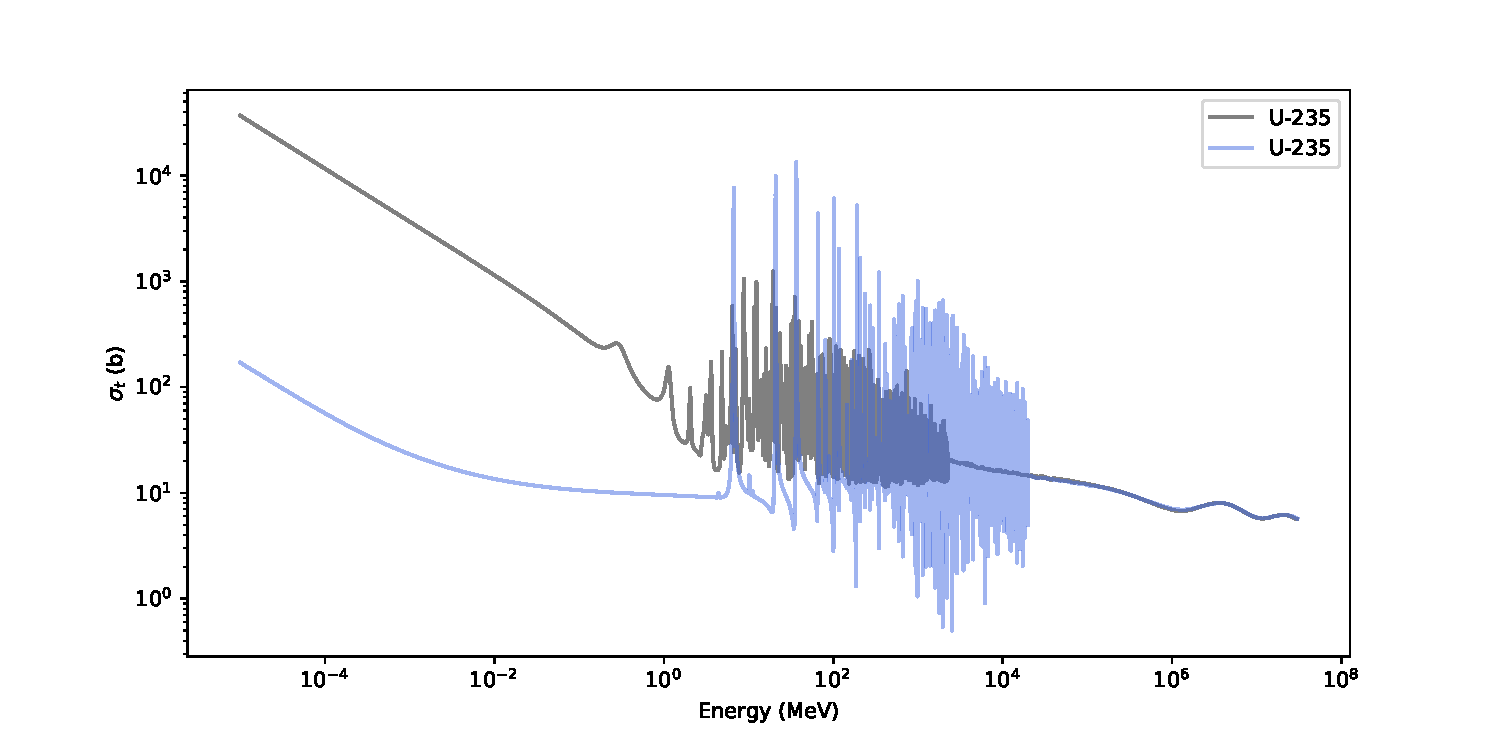
\includegraphics[width=0.85\linewidth]{\figpath/U235-8-XST}
                    \caption{Uranium 235 and 238 total microscopic cross sections as a function of energy. Data provided through the ENDF-8.0 nuclear reaction data library \cite{ENDF8}.}
                    \label{fig:NTT:Cross Section plot}
                \end{figure}

                The complicated dependence on energy would require hundreds of thousands of energy points to faithfully represent for the energies of interest in thermal reactors.
                Modeling of this many energy points in whole-core simulations would require too much memory.
                The multi-group approximation divides this energy space into several energy groups; within each group cross sections are averaged.
                The multi-group eigenvalue transport equation can be found by integrating the \cref{eq:NTT:Eigenvalue Transport Problem} over an energy energy interval $[E_{g}, E_{g-1})$.
                \begin{aequation}\label{eq:NTT:MGEV Transport Problem w/ Anisotropic XS}
                    \left[\dir\vdot\grad + \xst[\loc,\dir]\right]\aflux
                        = \rfourpi\Bigg[&\suml[\gprime=1][G]\intl[\fourpi]\xss[][\loc][\dir,\dirprime]\aflux[\loc][\dirprime][\gprime]\ddirprime \\
                        + &\frac{\spect}{\keff}\suml[\gprime=1][G]\nufis[\loc,\dir]\sflux[\loc]\Bigg]
                \end{aequation}
                \begin{equation*}
                    \forall\loc, \quad \forall\dir\in\fourpi,\quad \forall g\in\{1,2,\ldots,G\},
                \end{equation*}
                where the multi-group quantities are defined by
                \begin{subequations}\label{eqs:NTT:Multi-group Quantities Anisotropic}
                    \begin{equation}\label{eq:NTT:Multi-group Angular Flux}
                        \aflux \defined \intl[E_g][E_{g-1}]\AngularFlux(\loc,\dir,E)\dif{E},
                    \end{equation}
                    \begin{equation}\label{eq:NTT:Multi-group Spectrum}
                        \spect \defined \intl[E_g][E_{g-1}]\Spectrum(\loc,E)\dif{E},
                    \end{equation}
                    \begin{equation}\label{eq:NTT:Multi-group Total Cross Section Anisotropic}
                        \xst[\loc,\dir] \defined \frac{\intl[E_{g}][E_{g-1}]\CrossSection_{t}(\loc,E)\AngularFlux(\loc,\dir,E)\dif{E}}{\aflux},
                    \end{equation}
                    \begin{equation}\label{eq:NTT:Multi-group Fission Cross Section Anisotropic}
                        \nufis[\loc,\dir][g] \defined \frac{\intl[E_{g}][E_{g-1}]\nu\CrossSection_{f}(\loc,E)\AngularFlux(\loc,\dir,E)\dif{E}}{\aflux},
                    \end{equation}
                    \begin{equation}\label{eq:NTT:Multi-group Scattering Cross Section Anisotropic}
                        \xss[][\loc][\dir,\dirprime] \defined \frac{\intl[E_{g}][E_{g-1}]\intl[E_{\gprime}][E_{\gprime-1}]\CrossSection_{s}(\loc,\dirprime\vdot\dir,\Eprime\to E)\AngularFlux(\loc,\dirprime,\Eprime)\dif{\Eprime}\dif{E}}{\aflux[\loc][\dirprime][\gprime]}.
                    \end{equation}
                \end{subequations}

                By defining the cross sections in this way, no approximations have been made, and the reaction rates of each energy group are preserved.
                However, this approach has two issues: the cross sections are dependent on the angular flux which is not known \textit{a priori}, and have dependence on the neutron direction of flight.
                Generally, the dependence on the angular flux is addressed by solving a simplified problem to generate a continuous or fine-group neutron energy spectrum.
                This spectrum is then used to ``collapse'' the cross sections into coarser multi-group values \cite{Knott2010}.
                This introduces approximation into the transport equation.

                To eliminate the directional dependence of the multi-group cross sections, an additional approximation is made: isotropic angular flux spectrum,
                \begin{equation}\label{eq:NTT:Multi-group Isotropic Spectrum}
                    \AngularFlux(\loc,\dir,E) \approx \rfourpi\FluxSpectrum(\loc, E).
                \end{equation}
                Using this approximate angular flux as the weighting function for multi-group cross sections in \cref{eqs:NTT:Multi-group Quantities Anisotropic,eq:NTT:MGEV Transport Problem w/ Anisotropic XS} can be simplified to
                \begin{aequation}\label{eq:NTT:MGEV Transport Problem}
                    \left[\dir\vdot\grad + \xst\right]\aflux = \rfourpi\Bigg[&\suml[\gprime=1][G]\intl[\fourpi]\xss\aflux[\loc][\dirprime][\gprime]\ddirprime\\
                        + \frac{\spect}{\keff}&\suml[\gprime=1][G]\nufis\intl[\fourpi]\aflux[\loc][\dirprime][\gprime]\ddirprime\Bigg],
                \end{aequation}
                \begin{equation*}
                    \forall\loc, \quad \forall\dir\in\fourpi,\quad \forall g\in\{1,2,\ldots,G\},
                \end{equation*}
                where the approximated multigroup cross sections are defined as
                \begin{subequations}\label{eqs:NTT:Multi-group Cross Sections}
                    \begin{equation}\label{eq:NTT:Multi-group Total Cross Section}
                        \xst \defined \frac{\intl[E_{g}][E_{g-1}]\CrossSection_{t}(\loc,E)\FluxSpectrum(\loc,E)\dif{E}}{\intl[E_{g}][E_{g-1}]\FluxSpectrum(\loc,E)\dif{E}},
                    \end{equation}
                    \begin{equation}\label{eq:NTT:Multi-group Fission Cross Section}
                        \nufis[\loc][g] \defined \frac{\intl[E_{g}][E_{g-1}]\nu\CrossSection_{f}(\loc,E)\FluxSpectrum(\loc,E)\dif{E}}{\intl[E_{g}][E_{g-1}]\FluxSpectrum(\loc,E)\dif{E}},
                    \end{equation}
                    \begin{equation}\label{eq:NTT:Multi-group Scattering Cross Section}
                        \xss \defined \frac{\intl[E_{g}][E_{g-1}]\intl[E_{\gprime}][E_{\gprime-1}]\CrossSection_{s}(\loc,\dirprime\vdot\dir,\Eprime\to E)\FluxSpectrum(\loc,\Eprime)\dif{\Eprime}\dif{E}}{\intl[E_{\gprime}][E_{\gprime-1}]\FluxSpectrum(\loc,\Eprime)\dif{\Eprime}}.
                    \end{equation}
                \end{subequations}
            }
            \subsubsection{Spatial Discretization}{\label{sssec:NTT:Spatial Discretization}
                Nearly all computational transport methods involve some form of spatial discretization.
                Reactor designs include many different material regions, and nearly all simulation tools will discretize the spatial domain into these different material regions.
                Deterministic methods will generally apply a finer meshing within these material regions, into transport cells.
                For the purposes of this work, a cell $\mathcal{R}_i$ is indexed with $i$.
                A visualization of the material and hypothetical meshing for a single pin-cell are shown in \cref{fig:NTT:Pin Cell}.
                In deterministic codes, the typical assumption is that material properties (cross sections) are constant within each computational cell.

                \begin{figure}[h]
                    \centering
                    \begin{subfigure}[t]{0.45\linewidth}
                        \centering
                        \def\svgwidth{\linewidth}
                        \input{\figpath/PinCell.pdf_tex}
                        \caption{Material regions}
                        \label{fig:NTT:Pin Cell Materials}
                    \end{subfigure}%
                    \hfill
                    \begin{subfigure}[t]{0.45\linewidth}
                        \centering
                        \def\svgwidth{\linewidth}
                        \input{\figpath/PinCellMesh.pdf_tex}
                        \caption{Hypothetical computational cell mesh}
                        \label{fig:NTT:Pin Cell Mesh}
                    \end{subfigure}
                    \caption{Material and mesh spatial discretization examples for a single pin cell.}
                    \label{fig:NTT:Pin Cell}
                \end{figure}
            }
            \subsubsection{Directional Discretization}{\label{sssec:NTT:Directional Discretization}
                %%% Discrete Ordinates Quantities %%%
\DeclareDocumentCommand{\mprime}{}{m^{\prime}}
\DeclareDocumentCommand{\dirm}{ O{m} }{\dir_{#1}}
\DeclareDocumentCommand{\wt}{ O{m} }{\Weight_{#1}}

% Quadrature set
\DeclareDocumentCommand{\angquad}{ O{N} }{ \mathcal{M}_{#1} }

% Cross-Sections
\DeclareDocumentCommand{\xss}{ o O{\loc} O{ m^{\prime}\!\to m} O{\gprime\!\to g} }{
    \IfNoValueOrEmptyTF{#1}
    {\xs[s,#3][#2][#4]}
    {\xs[s,#1][#2][#4]}
}

% Flux
\DeclareDocumentCommand{\aflux}{ O{\loc} O{m} O{g}}{\ensuremath{\AngularFlux^{#3}_{#2}\!\left(#1\right)}}

% Source
\DeclareDocumentCommand{\source}{ O{\loc} O{m} O{g} }{\ensuremath{q^{#3}_{#2}\!\left(#1\right)}}


                Typically, the directional variable cannot be treated exactly in deterministic methods.
                There are two common methods of approximating behavior as a function of direction $\dir$:
                \begin{enumerate}
                    \item{\ac{PN} Expansion}
                    \item{\ac{SN}}
                \end{enumerate}

                Expansion in spherical harmonics, often referred to as \acs{PN}, is one of the oldest transport methods, where $N$ indicates the order of the expansion.
                In this method, the angular flux is expanded as a linear combination of spherical harmonics moments.
                The simplest expansion of order 1, reduces to the diffusion approximation.

                The \acf{SN} method is a discretization of the directional variable $\dir$; typically, the discrete direction values are determined using a set of quadrature points.
                \begin{subequations}\label{eqs:NTT:Directional Quadrature}
                    Let the $\angquad$ be the set of discrete directions, and weights,
                    \begin{equation}\label{eq:NTT:Directional Quadrature Definition}
                        \angquad \defined \left\{\dirm \in \{\dir_1,\dir_2,\ldots,\dir_N\}, \wt \in \{\wt[1], \wt[2], \ldots,\wt[N]\}\right\},
                    \end{equation}
                    such that a directional integration can be approximated as
                    \begin{equation}\label{eq:NTT:Directional Quadrature Integration}
                        \intl[\fourpi]f(\dir)\ddir \approx \fourpi\suml[m\in\angquad]\wt f(\dirm),
                    \end{equation}
                    where
                    \begin{equation}\label{eq:NTT:Directional Quadrature Weight Sum}
                        \suml[m\in\angquad]\wt = 1.
                    \end{equation}
                \end{subequations}

                There are two common forms of quadrature sets that are commonly used in transport calculations: level-symmetric and product quadratures.
                The level-symmetric quadratures include directions that are evenly distributed over the unit-sphere; this is optimal in situations where each direction has similar variation.
                However, typical reactor designs have significantly less variation in the axial ($z$) direction which fuel rods are oriented along.
                In this situation, neutrons with directions close to the $z$-axis are modeled poorly because there are few azimuthal angles at these polar levels, as is demonstrated in \cref{fig:NTT:S8 Quadrature}.
                These steep polar angles are important in reactor analysis due to self-shielding effects, which are strongly dependent on polar angle. % [CITATION].

                Product quadratures are generated by a multiplicative combination of separate quadrature sets in the azimuthal and polar directions.
                The azimuthal quadrature set in generated over the domain $[0,2\pi]$, while the polar quadrature set is generated for the polar cosine $\mu$ over the domain $[-1,1]$.
                This quadrature generation technique does not suffer from the same issue for steep polar directions, as each polar level has the same number of azimuthal directions.
                A common choice for the azimuthal quadrature generation in the Chebyshev quadrature set, which gives evenly spaced azimuthal angles.
                The polar cosine quadrature set typically uses a Gauss-Legendre quadrature set, or an optimized quadrature set such as the Tabuchi-Yamamoto quadrature \cite{TabuchiYamamotoQuad}.
                \Cref{fig:NTT:ChebyshevGauss Quadrature} shows an example of a product quadrature's set of directions using a Chebyshev azimuthal quadrature and Gauss-Legendre polar quadrature.

                \begin{figure}[h]
                    \centering
                    \begin{subfigure}[t]{0.45\linewidth}
                        \centering
                        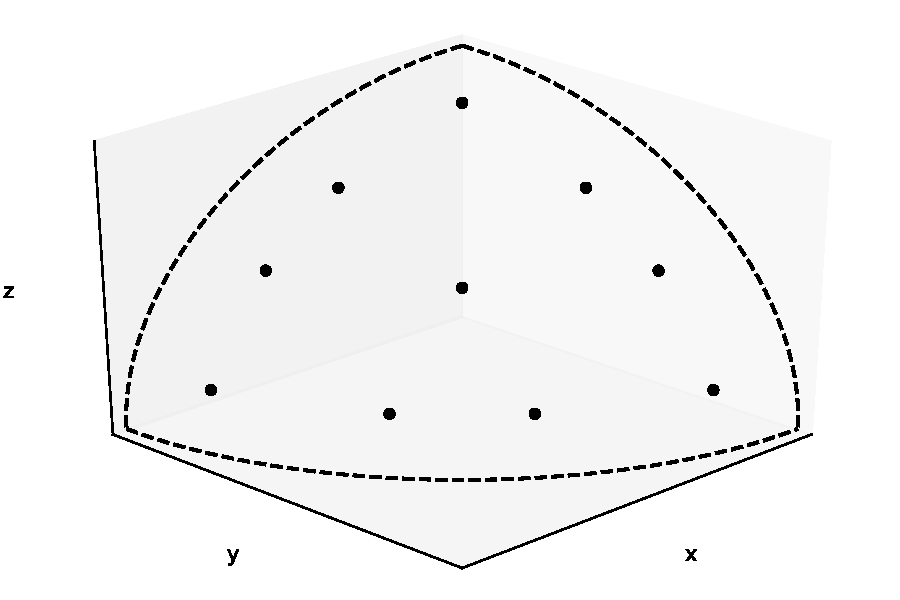
\includegraphics[width=\linewidth]{S8-Quadrature}
                        \caption{Level-Symmetric Quadrature ($S_8$)}
                        \label{fig:NTT:S8 Quadrature}
                    \end{subfigure}%
                    \hfill
                    \begin{subfigure}[t]{0.45\linewidth}
                        \centering
                        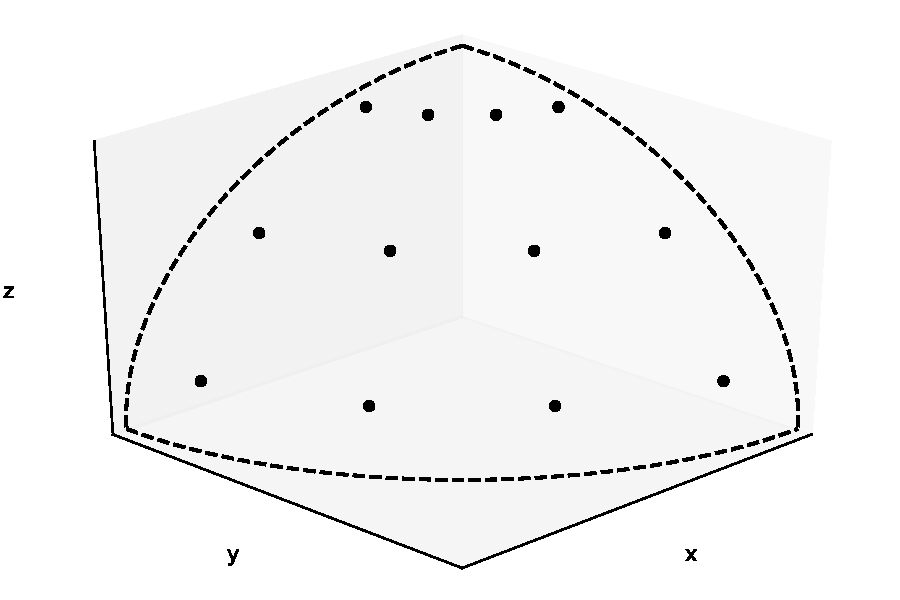
\includegraphics[width=\linewidth]{ChebyshevGauss}
                        \caption{Chebyshev-Gauss Product Quadrature with 4 azimuthal and 3 polar angles}
                        \label{fig:NTT:ChebyshevGauss Quadrature}
                    \end{subfigure}
                    \caption{(a) Level-Symmetric and (b) product quadrature direction set examples shown for a single octant of the unit-sphere.}
                    \label{fig:NTT:Quadrature Examples}
                \end{figure}
            }
            \subsubsection{The Method of Characteristics}{\label{sssec:NTT:MOC}
                The \acf{MOC} is a technique used in mathematics to solve \acp{PDE}, by transforming a \ac{PDE} into a system of \acp{ODE}.
                The method was first applied to the neutron transport problem by \citeauthor{Askew1972} in 1972 \cite{Askew1972}, but only began to see real use in the 1980's \cite{Halsall1980}.
                The \ac{MOC} transforms the transport equation into the characteristic form, by examining the equation along straight neutron paths through the spatial domain.

                Typically, the spatial domain is discretized into cells that have uniform material data (cross sections).
                By examining the equation along one of these characteristic ``tracks'' or ``rays'', the average angular flux along the track within a cell can be calculated.
                The scalar flux can then be found by collecting the average angular flux along all tracks passing through this region, in a numerical integration over space and angle.

                Like the \ac{CP} method, \ac{MOC} is able to handle completely arbitrary geometry; however, it is also able to account for anisotropic scattering.
                Additionally, the \ac{MOC} does not produce the large matrices in realistic applications as the \ac{CP} method does.
                For problems that contain more than a few hundred cells, the \ac{MOC} is generally preferred over \ac{CP} methods \cite{Hebert2010}.

                The \ac{CDP} is a method similar to both \ac{CP} method and the \ac{MOC} \cite{Hong1999,Liu2014}; the major difference from \ac{CP} is that \ac{CDP} only couples together cells are traversed by characteristic tracks.
                This significantly cuts down on the computational resources required by traditional \ac{CP} methods.
                This method has also shown improvements over \ac{MOC} in cases with few unique geometries and constant material properties throughout the simulation; however these conditions are not applicable in problems of interest to industry.

                The \ac{MOC} is the primary subject of this thesis work.
                As such, \cref{ch:The Method of Characteristics} has been devoted to the details of the method, and \cref{ch:Ray-Tracing} expands upon the details of ray-tracing that is central to the \ac{MOC}.
            }
        }
    }
    \section{Source Iteration}{\label{sec:NTT:Source Iteration}
        Generally, the $k$-eigenvalue transport problems, introduced in \cref{sec:NTT:k-Eigenvalue Problems}, are solved iteratively.
        Given an initial guess for the $k$-eigenvalue, boundary conditions, and interior flux-moments, an estimate of the source can be computed.
        A transport ``sweep'' can be performed, in which updated boundary conditions and flux-moments are computed.
        Given these updated flux-moments a new estimate of the eigenvalue can be calculated.
        This process can be repeated until the eigenvalue and flux-moments are converged within some tolerance.
        For simplicity, this process is shown for a isotropic mono-energetic, continuous-space, one-dimensional transport problem in \cref{alg:NTT:Source Iteration}.

        \begin{algorithm}[ht]
            \centering
            \caption{Source Iteration algorithm for the $k$-eigenvalue transport problem.}
            \label{alg:NTT:Source Iteration}
            \begin{algorithmic}[1]
                \State{Begin iteration $j$ with a known boundary conditions, scalar flux estimate, $\ScalarFlux^{(j)}(x)$, and a $k$-eigenvalue estimate, $\keff^{j}$.}
                \State{Perform a transport sweep:
                    \begin{equation}\label{eq:NTT:Source Iteration:Transport Sweep}
                        \left[\PolarCos\pderiv{}{x} + \CrossSection_t(x)\right]\AngularFlux^{(j+1)}(x,\PolarCos) = \frac{1}{2}\left[\CrossSection_s(x) + \frac{1}{\keff^{(j)}}\nu\CrossSection_f(x)\right]\ScalarFlux^{(j)}(x),
                    \end{equation}
                    \begin{equation*}
                        \forall x\in [0,X], \quad \forall\PolarCos \in [-1, 1].
                    \end{equation*}
                }
                \State{Update the scalar flux, and the eigenvalue for the next iteration:
                    \begin{subequations}\label{eqs:NTT:Source Iteration:Update}
                        \begin{equation}\label{eq:NTT:Source Iteration:Scalar Flux Update}
                            \ScalarFlux^{(j+1)}(x) = \intl[-1][1]\AngularFlux^{(j+1)}(x,\PolarCos)\dif{\PolarCos} \frac{\Phi_0}{\frac{1}{X}\intl[0][X]\intl[-1][1]\AngularFlux^{(j+1)}(x',\PolarCos)\dif{\PolarCos}\dif{x'}},
                        \end{equation}
                        \begin{equation}\label{eq:NTT:Source Iteration:Eigenvalue Update}
                            \keff^{(j+1)} = \frac{\intl[0][X]\nu\CrossSection_f\ScalarFlux^{(j+1)}(x)\dif{x}}{\intl[0][X]\CrossSection_a\ScalarFlux^{(j+1)}(x)\dif{x}}.
                        \end{equation}
                    \end{subequations}
                }
                \State{Repeat steps 1. - 3. until sufficient convergence.}
            \end{algorithmic}
        \end{algorithm}

        \subsection{Transport Acceleration}{\label{ssec:NTT:Transport Acceleration}
            While \cref{alg:NTT:Source Iteration} is valid, it typically converges very slowly, requiring many iterations to get reasonable results.
            In full-core calculations, a single transport sweep can become computationally expensive and using \cref{alg:NTT:Source Iteration} is not feasible.
            There has been considerable effort in developing methods that accelerate transport calculations by using a lower-order calculation, typically based on the diffusion approximation.
            While other acceleration methods exist \cite{Hebert2017}, the most common are \ac{NDA} methods \cite{Smith2002}, typically using the \ac{CMFD} method \cite{Smith1983}.

            The \ac{CMFD} acceleration method has been shown to significantly reduce computational transport run-times \cite{Smith2002,Anistratov2011,Collins2016}.
            Improvements upon the original \ac{CMFD} formulation \cite{Smith1983}.
            The p\ac{CMFD} method preserves partial currents rather than net currents, and has been shown to be unconditionally stable for transport problems at fixed conditions \cite{Cho2002}.
            The od\ac{CMFD} method generalizes the \ac{CMFD} and p\ac{CMFD} methods by adding an artificial term to the diffusion coefficient, and has faster convergence properties than p\ac{CMFD} \cite{Zhu2016}.

            Utilization of \ac{CMFD} acceleration in transport calculations with \ac{TH} feedback has not had the favorable stability and convergence properties as calculations without feedback \cite{Kochunas2017}.
            Many transport codes have required under-relaxation of the scalar flux in the iteration schemes for stability in these calculations; there is ongoing research investigating a less ad-hoc approach \cite{Kochunas2017}.
            This instability and convergence slow-down in problems with feedback has prevented full utilization of more advanced multi-level solvers \cite{Yee2018a}.

            % \subsubsection{Coarse Mesh Finite Difference}{\label{sssec:NTT:CMFD}

            % }
        }
    }
    % References
    % \printbibliography
}
    \chapter{The Method of Characteristics}{\label{ch:The Method of Characteristics}
    %%% Multi-group Energy quantities %%%
\DeclareDocumentCommand{\gprime}{}{g^{\prime}}
% Cross-sections
\DeclareDocumentCommand{\xs}{ O{t} O{\loc} O{g}}{\ensuremath{\CrossSection_{#1}^{#3}(#2)}}
\DeclareDocumentCommand{\xst}{ O{\loc} O{g} }{\xs[t][#1][#2]}
\DeclareDocumentCommand{\xsa}{ O{\loc} O{g} }{\xs[a][#1][#2]}
\DeclareDocumentCommand{\xsf}{ O{\loc} O{\gprime} }{\xs[f][#1][#2]}
\DeclareDocumentCommand{\xss}{ o O{\loc} O{\dirprime\vdot\dir} O{\gprime \to g} }{
    \IfNoValueOrEmptyTF{#1}
    {\xs[s][#2,#3][#4]}
    {\xs[s,#1][#2][#4]}
}
\DeclareDocumentCommand{\spect}{ O{\loc} O{g} }{\ensuremath{\Spectrum^{#2}(#1)}}
\DeclareDocumentCommand{\nufis}{ O{\loc} O{\gprime} }{ \ensuremath{\nu\xsf[#1][#2]}}
\DeclareDocumentCommand{\D}{ O{\loc} O{g} }{\ensuremath{D^{#2}(#1)}}

% Flux
\DeclareDocumentCommand{\aflux}{ O{\loc} O{\dir} O{g} }{\ensuremath{\AngularFlux^{#3}(#1,#2)}}
\DeclareDocumentCommand{\sflux}{ O{\loc} O{\gprime} }{\ensuremath{\ScalarFlux^{#2}(#1)}}
\DeclareDocumentCommand{\current}{ O{\loc} O{g} }{\ensuremath{\Current^{#2}(#1)}}
\DeclareDocumentCommand{\fluxmoma}{ O{\ell} O{n} O{\loc} O{g} }{\ensuremath{\ScalarFlux^{#2,#4}_{#1}(#3)}}

% Source
\DeclareDocumentCommand{\source}{ O{\loc} O{\dir} O{g} }{\ensuremath{q^{#3}(#1,#2)}}
\DeclareDocumentCommand{\sourcemoma}{ O{\ell} O{n} O{\loc} O{g} }{\ensuremath{q^{#2,#4}_{#1}(#3)}}

    %%% Discrete Ordinates Quantities %%%
\DeclareDocumentCommand{\mprime}{}{m^{\prime}}
\DeclareDocumentCommand{\dirm}{ O{m} }{\dir_{#1}}
\DeclareDocumentCommand{\wt}{ O{m} }{\Weight_{#1}}

% Quadrature set
\DeclareDocumentCommand{\angquad}{ O{N} }{ \mathcal{M}_{#1} }

% Cross-Sections
\DeclareDocumentCommand{\xss}{ o O{\loc} O{ m^{\prime}\!\to m} O{\gprime\!\to g} }{
    \IfNoValueOrEmptyTF{#1}
    {\xs[s,#3][#2][#4]}
    {\xs[s,#1][#2][#4]}
}

% Flux
\DeclareDocumentCommand{\aflux}{ O{\loc} O{m} O{g}}{\ensuremath{\AngularFlux^{#3}_{#2}\!\left(#1\right)}}

% Source
\DeclareDocumentCommand{\source}{ O{\loc} O{m} O{g} }{\ensuremath{q^{#3}_{#2}\!\left(#1\right)}}

    %%% MOC quantities %%%
% Geometric
\DeclareDocumentCommand{\Length}{}{s}
\DeclareDocumentCommand{\NormalizedLength}{}{t}
\DeclareDocumentCommand{\len}{ O{} }{\Length_{#1}}
\DeclareDocumentCommand{\segl}{ O{mki} }{\Length_{#1}}
\DeclareDocumentCommand{\nlen}{ O{m} }{\NormalizedLength_{#1}}
\DeclareDocumentCommand{\nsegl}{ O{mki} }{\NormalizedLength_{#1}}

\DeclareDocumentCommand{\centroid}{ O{\loc} O{i} }{#1_{#2}^{\text{c}}}
\DeclareDocumentCommand{\locIn}{ O{\loc} O{mki} }{{#1}_{#2}^{\text{in}}}
\DeclareDocumentCommand{\locOut}{ O{\loc} O{mki} }{{#1}_{#2}^{\text{out}}}
\DeclareDocumentCommand{\locCent}{ O{\loc} O{mki} }{{#1}_{#2}^{\text{c}}}
\DeclareDocumentCommand{\M}{ o O{i}}{%
    \IfNoValueOrEmptyTF{#1}
        {\vec{M}_{#2}}
        {M_{#2,#1}}
}
\DeclareDocumentCommand{\C}{o O{i} O{g}}{%
    \IfNoValueOrEmptyTF{#1}
        {\vec{C}_{#2}^{#3}}
        {C_{#2,#1}^{#3}}
}


% Integration
\DeclareAutoPairedDelimiter{\MOCTrackIntegral}{\langle}{\rangle_{mki}}
\DeclareAutoPairedDelimiter{\MOCSingleAngleIntegral}{\langle}{\rangle_{mi}}
\DeclareAutoPairedDelimiter{\MOCIntegral}{\langle}{\rangle_{i}}

% Cross-sections
\DeclareDocumentCommand{\xs}{ O{t} O{i} O{g}}{\ensuremath{\CrossSection_{#1,#2}^{#3}}}
\DeclareDocumentCommand{\xst}{ O{i} O{g} }{\xs[t][#1][#2]}
\DeclareDocumentCommand{\xsa}{ O{i} O{g} }{\xs[a][#1][#2]}
\DeclareDocumentCommand{\xsf}{ O{i} O{\gprime} }{\xs[f][#1][#2]}
\DeclareDocumentCommand{\xss}{ o O{i} O{m'\to m} O{\gprime \to g} }{
    \IfNoValueOrEmptyTF{#1}
    {\xs[s][#2,#3][#4]}
    {\xs[s,#1][#2][#4]}
}

\DeclareDocumentCommand{\spect}{ O{i} O{g} }{\ensuremath{\Spectrum^{#2}_{#1}}}
\DeclareDocumentCommand{\nufis}{ O{i} O{\gprime} }{ \ensuremath{\nu\xsf[#1][#2]}}
\DeclareDocumentCommand{\D}{ O{i} O{g} }{\ensuremath{D^{#2}_{#1}}}
\DeclareDocumentCommand{\opt}{ O{m} O{g} }{\OpticalThickness_{#1}^{#2}}
\DeclareDocumentCommand{\segopt}{ O{mki} O{g} }{\opt[#1][#2]}

% MOC Parameters
\DeclareDocumentCommand{\tA}{ O{a} }{\ensuremath{\delta\!A_{#1}}}
\DeclareDocumentCommand{\Weight}{}{w}
\DeclareDocumentCommand{\wt}{ O{m} }{\Weight_{#1}}
\DeclareDocumentCommand{\wtbar}{ O{m} }{\overline{\Weight}_{#1}}
\DeclareDocumentCommand{\renorm}{ O{i} }{\ensuremath{\xi_{#1}}}

% Flux
\DeclareDocumentCommand{\aflux}{ O{mki} O{g} O{\len} }{
    \IfNoValueOrEmptyTF{#3}
    {\AngularFlux^{#2}_{#1}}
    {\ensuremath{\AngularFlux^{#2}_{#1}\!\left(#3\right)}}
}
\DeclareDocumentCommand{\afluxin}{ O{mki} O{g} }{\AngularFlux^{#2,\text{in}}_{#1}}
\DeclareDocumentCommand{\afluxout}{ O{mki} O{g} }{\AngularFlux^{#2,\text{out}}_{#1}}
\DeclareDocumentCommand{\sflux}{ O{g} O{i} }{\ScalarFlux_{#2}^{#1}}
\DeclareDocumentCommand{\current}{ O{i} O{g} }{\Current^{#2}_{#1}}
\DeclareDocumentCommand{\tfluxF}{ O{mki} O{g} }{ \overline{\AngularFlux}_{#1}^{#2} }          % Average flux-moment along track
\DeclareDocumentCommand{\tfluxL}{ O{mki} O{g} }{  \widehat{\AngularFlux}_{#1}^{#2} }          % Linear flux-moment along track
\DeclareDocumentCommand{\dflux}{ O{mki} O{g} }{ \Delta\AngularFlux_{#1}^{#2} }                % Difference of angular flux along track
\DeclareDocumentCommand{\sfluxF}{ O{i} O{g} }{ \overline{\ScalarFlux}_{#1}^{#2} }             % Average scalar flux
% \DeclareDocumentCommand{\sfluxL}{ o O{i} O{g} }{ % Linear expansion coeff (Scalar Flux)
%     \IfNoValueOrEmptyTF{#1}
%         {\lvec{\widehat{\ScalarFlux}}_{#2}^{#3}}
%         {\widehat{\ScalarFlux}_{#2,#1}^{#3}}
% }
\DeclareDocumentCommand{\sfluxL}{ O{i} O{g} o }{ % Linear expansion coeff (Scalar Flux)
    \IfNoValueOrEmptyTF{#3}
        {\lvec{\widehat{\ScalarFlux}}_{#1}^{#2}}
        {\widehat{\ScalarFlux}_{#1,#3}^{#2}}
}
% \DeclareDocumentCommand{\sfluxL}{ m O{i} O{g} }{\widehat{\ScalarFlux}_{#2,#1}^{#3} }          % Linear expansion coeff (Scalar flux)
\DeclareDocumentCommand{\afluxmom}{ O{\ell} O{n} O{i} O{\gprime} }{\FluxMoment_{#3,#1}^{#4,#2}}

% Source
\DeclareDocumentCommand{\source}{ O{mki} O{g} O{\len} }{\ensuremath{q^{#2}_{#1}\!\left(#3\right)}}
\DeclareDocumentCommand{\tsrcF}{ O{mki} O{g} }{ \overline{q}_{#1}^{#2} }          % Average source along track
\DeclareDocumentCommand{\tsrcL}{ O{mi} O{g} }{ \widehat{q}_{#1}^{#2} }          % Linear source along track
\DeclareDocumentCommand{\src}{ O{i} O{g} }{ \Source_{#1}^{#2}}                          % Generic source
\DeclareDocumentCommand{\srcF}{ O{i} O{g} }{ q_{#1}^{#2} }             % Average source
\DeclareDocumentCommand{\srcL}{ o O{i} O{g} }{ % Linear expansion coeff (Source)
    \IfNoValueOrEmptyTF{#1}
        {\lvec{\widehat{q}}_{#2}^{#3}}
        {\widehat{q}_{#2,#1}^{#3}}
}

% Linear source operators / functions
\DeclareDocumentCommand{\FluxToSource}{ O{g} }{\mathcal{S}^{#1}}
    \def\figpath{chapters/03/figures/}
    \graphicspath{ {\figpath} }

    \section{Fundamentals}{\label{sec:MOC:Fundamentals}
        The \acf{MOC} is a technique used in mathematics to solve \acp{PDE}, by transforming a \ac{PDE} into a system of \acp{ODE}.
        The method was first applied to the neutron transport equation by \citeauthor{Askew1972} in 1972 \cite{Askew1972}, but only began to see real use in the 1980's \cite{Halsall1980}.
        The \ac{MOC} transforms the transport equation into the characteristic form, by following the equation along straight neutron paths through the spatial domain.
        For brevity, the derivation of this method will begin with the multi-group \ac{SN} $k$-eigenvalue transport equation with spatially discretized mesh with constant material properties within each cell.
        \begin{equation}\label{eq:MOC:SSMGFS Transport}
            \left[\dirm\vdot\grad + \xst\right]\aflux[mi][g][\loc] = \rfourpi\source[mi][g][\loc],
        \end{equation}
        \begin{equation*}
            \forall\loc\in\Region, \quad \forall m \in \angquad, \quad \forall i, g,
        \end{equation*}
        where $\Region$ is the spatial cell, $\angquad$ is the directional quadrature, as described in \cref{sssec:NTT:Directional Discretization}, and the fixed-source, $
        \source[mi][g][\loc]$ can be found by applying the discrete-to-moment operator, $\FluxToSource$, defined by
        \begin{equation}\label{eq:MOC:LSA:Flux To Source Operator}
          \FluxToSource(f) \defined
            \suml[\gprime]\suml[\ell=0][L]\suml[n=-\ell][\ell]\SH[\ell][n][\dirm]\xss[\ell]f^{\ell,\gprime}_{n,i}(\loc)
            + \frac{\spect}{\keff}\suml[\gprime]\nufis f^{\gprime}_{i}(\loc),
        \end{equation}
        to get
        \begin{equation}\label{eq:MOC:Source}
            \source[mi][g][\loc] \defined
                \left[\suml[\gprime]\suml[\ell=0][L]\suml[n=-\ell][\ell]\SH\xss[\ell]\afluxmom(\loc) + \frac{\spect}{\keff}\suml[\gprime]\nufis\sflux[\gprime](\loc)\right].
        \end{equation}

        Consider a point, $\loc_0$, and a line passing through this point in direction $\dirm$.
        Any location along this \emph{characteristic} line (also referred to as a ray, or track), can be described as
        \begin{equation}\label{eq:MOC:Characteristic Ray}
            \loc = \loc_0 + \len\dirm,
        \end{equation}
        where $\len$ is the distance along the track from $\loc_0$.
        Applying this transformation, \cref{eq:MOC:SSMGFS Transport} is put into the characteristic form
        \begin{equation}\label{eq:MOC:Characteristic Form Deriv 1}
            \left[\deriv{}{\len} + \xst\right]\aflux[mi][g][\loc_0 + \len\dirm] = \rfourpi\source[mi][g][\loc_0 + \len\dirm].
        \end{equation}
        As stated in \cref{sec:NTT:Neutron Transport Equation}, reactor physicists are generally interested in spatially and directionally integrated angular flux quantities rather than the angular flux along a single path.
        It is thus typical in the \ac{MOC} to have many different characteristic tracks through our problem; in this work separate tracks will be subscripted with the index $k$.
        The track is broken up into track-segments by considering the segments contained within each computational cell.
        The characteristic form of the transport equation then becomes
        \begin{equation}\label{eq:MOC:MOC Equation Generic}
            \left[\deriv{}{\len} + \xst\right]\aflux = \rfourpi\source[mi][g][\len],
        \end{equation}
        \begin{equation*}
            \forall \len \in [0,\segl], \forall m\in\angquad, \forall i,k,g,
        \end{equation*}
        where $\segl$ is the total length of the track-segment, as depicted in \cref{fig:MOC:MOC Coordinate System}.

        \begin{figure}[h]
            \centering
            \def\svgwidth{0.4\linewidth}
            \input{\figpath/MOCCoordinateSystem.pdf_tex}
            \caption{Depiction of a single characteristic track through a cell $i$.}
            \label{fig:MOC:MOC Coordinate System}
        \end{figure}

        \Cref{eq:MOC:MOC Equation Generic} can be solved analytically along a characteristic track-segment using an integrating factor,
        \begin{equation}\label{eq:MOC:Integrating Factor}
            M(\len) = \exp\!\left(\intl[0][\len]\xst\dif{s'}\right) = \exp\!\left(\opt\right),
        \end{equation}
        where the \emph{optical thickness}, $\opt$, is defined by
        \begin{equation}\label{eq:MOC:Optical Thickness Definition}
            \opt \defined \xst\len.
        \end{equation}
        Using this integrating factor, the generic solution to the \ac{MOC} equation, given in \cref{eq:MOC:MOC Equation Generic}, is
        \begin{equation}\label{eq:MOC:MOC Generic Solution}
            \aflux = \afluxin\exp\!\left(-\opt\right) + \intl[0][\len]\rfourpi\source[mi][g][\len']\exp\!\left(-\xst\left[\len-\len'\right]\right)\dif{s'},
        \end{equation}
        where $\afluxin$ is the incident angular flux, $\aflux[mki][g][0]$.
        If a source shape is provided, \cref{eq:MOC:MOC Generic Solution} can be evaluated for every track-segment in the problem.
        The next subsection introduces formal methods to approximate the integration of quantities over both space and direction.
        These procedures can be used to determine the scalar flux or other quantities necessary in \ac{MOC} calculations.

        \subsection{Track-Based Integration}{\label{ssec:MOC:Track-Based Integration}
            Determining the angular flux along a single characteristic track is typically not very useful for reactor physics calculations.
            It is most often necessary to evaluate reaction rates, and therefore the scalar flux through integration of the angular flux.
            This section aims to provide a formal basis for the integration process used in the \ac{MOC} for transport calculations.

            \begin{figure}[h]
                \centering
                \def\svgwidth{0.4\linewidth}
                \input{\figpath/MOCTracks.pdf_tex}
                \caption{Example characteristic tracks (2D) through a cell for a single direction.}
                \label{fig:MOC:MOC Tracks}
            \end{figure}

            The \ac{MOC} is based on the \acf{SN} approximation; integration over the directional variable simply becomes a quadrature integration:
            \begin{equation}\label{eq:MOC:Directional Quadrature Integration}
                \intl[\fourpi]f(\dir)\ddir \approx \fourpi\suml[m]\wt[m]f(\dirm).
            \end{equation}
            Within a cell, $\Region$, there are many characteristic track-segments for each direction in the directional quadrature, as is shown for a single direction in \cref{fig:MOC:MOC Tracks}.
            Thus, the spatial discretization is different for each direction, and spatial integration is linked with directional integration.
            For a single direction, the integration over the spatial domain can be approximated by the weighted summation of track-averaged values, with the weight being equal to the area of the track-segment.
            The average value of a function, $f(\loc,\dirm)$, along a track-segment is denoted as
            \begin{equation}\label{eq:MOC:Track-Averaged Definition UnRenormalized}
                \MOCTrackIntegral{f(\loc,\dirm)} \defined \frac{1}{\segl}\intl[0][\segl]f(\len,\dirm)\dif{\len},
            \end{equation}
            where $\segl$ is the total length of the track-segment.
            The spatial integration for a single direction becomes
            \begin{equation}\label{eq:MOC:Spatial Averaging Definition UnRenormalized}
                \frac{1}{V_i}\intl[\loc\in\Region]f(\loc,\dirm)\dif^3{\loc} \approx \MOCSingleAngleIntegral{f(\loc,\dirm)} \defined \frac{1}{V_i}\suml[k]\tA[mki]\segl\MOCTrackIntegral{f(\loc,\dirm)} ,
            \end{equation}
            where $\tA[mki]$ is the cross-sectional area of the track (width in 2-D).
            In this notation, the integral is divided by the volume such that $\MOCSingleAngleIntegral{f}$ is approximately the mean value in the region, for the direction $\dirm$.
            Finally, an integration over both space and angle can be defined as
            \begin{equation}\label{eq:MOC:Spatial and Directional Integration Definition}
                \MOCIntegral{f(\loc,\dir)} = \fourpi\suml[m]\wt[m]\MOCSingleAngleIntegral{f(\loc,\dirm)}.
            \end{equation}

            These integrations have been expressed as 3-D \ac{MOC} equations.
            For 2-D calculations, the form remains the same, except that in \cref{eq:MOC:Spatial Averaging Definition UnRenormalized}, which requires a scaling factor on the cell volume (now area):
            \begin{equation}
              \label{eq:MOC:Spatial Averaging Definition UnRenormalized 2D}
              \frac{1}{V_i}\intl[\loc\in\Region]f(\loc,\dirm)\dif^3{\loc} \approx \MOCSingleAngleIntegral{f(\loc,\dirm)} \defined \frac{\sin(\Polar_p)}{V_i}\suml[k]\tA[mki]\segl\MOCTrackIntegral{f(\loc,\dirm)}
            \end{equation}
        }
        \subsection{Track-Length Renormalization}{\label{sec:MOC:Track-Length Renormalization}
            In general, the spatial integration described in \cref{ssec:MOC:Track-Based Integration} does not preserve the cell volume; this is visually apparent in \cref{fig:MOC:MOC Tracks}.
            In order to preserve spatial volumes within a cell, track-lengths are often ``renormalized''.
            There are three renormalization methods which become obvious through the notation presented in \cref{ssec:MOC:Track-Based Integration}:
            \begin{enumerate}
                \item{segment-volume preservation}
                \item{direction-volume preservation}
                \item{volume preservation}
            \end{enumerate}

            Track-length renormalization involves adjusting the lengths of track-segments such that volume is preserved.
            Let us define a renormalization factor, $\renorm[mki]$, such that the renormalized track-length is given by
            \begin{equation}\label{eq:MOC:Track-Length Renormalization}
                \nsegl = \renorm[mki]\segl.
            \end{equation}
            The spatial integration schemes given by \cref{eq:MOC:Track-Averaged Definition UnRenormalized,eq:MOC:Spatial Averaging Definition UnRenormalized} become
            \begin{subequations}\label{eq:MOC:Renormalized Spatial Integration Definition}
                \begin{equation}\label{eq:MOC:Renormalized Track-Averaged Definition}
                    \MOCTrackIntegral{f(\loc,\dirm)} \defined \frac{1}{\nsegl}\intl[0][\nsegl]f(\len,\dirm)\dif{\nlen},
                \end{equation}
                and
                \begin{equation}\label{eq:MOC:Renormalized Spatial Averaging Definition}
                    \MOCSingleAngleIntegral{f(\loc,\dirm)} \defined \frac{1}{V_i}\suml[k]\tA[mki]\nsegl\MOCTrackIntegral{f(\loc,\dirm)},
                \end{equation}
                where the spatial variable $\loc$ can now be written as a function of the renormalized track-distance, $\nlen$, as
                \begin{equation}\label{eq:MOC:Renormalized Location Variable}
                    \loc =  \locIn + \nlen\dirm / \renorm[mki],
                \end{equation}
                where $\locIn$ is the starting point of the track-segment.
            \end{subequations}

            Segment-volume preservation is a renormalization method in which the track-length is adjusted such that the analytic volume within the cross-sectional area of each track-segment is preserved.
            This renormalization technique is the most ``correct'' method of renormalization, but is very expensive as each track is renormalized separately.
            It is also more difficult to implement, as the analytic area of each track-segment must be found.
            To the best of our knowledge, this method is not implemented in any production-level \ac{MOC} code.

            Direction-volume preservation is the next ``most-correct'' renormalization technique.
            In this method, every mono-directional spatial integration should preserve the cell volume, i.e.
            \begin{equation}\label{eq:MOC:Angle-Volume Preservation}
                \MOCSingleAngleIntegral{1} = 1.
            \end{equation}
            This constraint leads to the renormalization factor given by
            \begin{equation}\label{eq:MOC:Direction-Dependent Renormalization}
                \renorm[mi] = \frac{V_i}{\suml[k]\tA[mki]\segl}.
            \end{equation}
            This method is significantly less expensive in terms of memory, computational time, and difficulty of implementation.

            The simplest renormalization technique, volume preservation, only preserves the volume over the spatial and directional integration, i.e.
            \begin{equation}\label{eq:MOC:Volume Preservation}
                \MOCIntegral{1} = \fourpi.
            \end{equation}
            This constraint leads to the renormalization factor given by
            \begin{equation}\label{eq:MOC:Region Renormalization}
                \renorm[i] = \frac{V_i}{\suml[m]\wt[m]\suml[k]\tA[mki]\segl}.
            \end{equation}

            Renormalization is not the only technique used for volume preservation.
            Another method is to use the numerical volume, $\suml[k]\tA[mki]\segl$ in place of $V_i$ in \cref{eq:MOC:Spatial Averaging Definition UnRenormalized}.
            This seems to be a more consistent method; however, a detailed comparison of these methods has not taken place, to the best of our knowledge.
            The renormalization technique generally seems to be the faster approach, and is the approach used in MPACT \cite{Collins2016}, which is used extensively in this work.
        }
    }
    \section{The Flat-Source Approximation}{\label{sec:MOC:FSA}
        The simplest approximation to the spatial shape of the source, $\source[mi][g][\loc]$, within each cell is the \acf{FSA}.
        The \ac{MOC} has been widely used in lattice physics and neutron transport codes \cite{Knott2010}, many of which have utilized the \ac{FSMOC} \cite{Halsall1980,Hong1998,Saji2000,Smith2002,Sugimura2006,Masiello2008,Boyd2014,Collins2016}.

        \subsection{Derivation}{\label{ssec:MOC:FSA:Derivation}
            The \ac{FSA} is simply the assumption that within each cell, $\Region$, the source, $\source[mi][g][\loc]$, is uniform.
            This can be expressed as
            \begin{equation}\label{eq:MOC:FSA:Source Shape}
                \source[mi][g][\loc] \approx \srcF[mi] = \srcF + \suml[\ell=0][L]\suml[n=-\ell][\ell]\SH[\ell][n][\dirm]\srcF[i,\ell][g,n]
            \end{equation}
            Thus, to get a source in this form, \cref{eq:MOC:Source} requires that the region averaged scalar flux and higher-order angular moments (up to order $L$) be determined.
            In mathematical terms, the flat-source can be determined as
            \begin{equation}\label{eq:MOC:FSA:Source Computation}
                \srcF[mi] =
                    \left[
                        \suml[\gprime]\suml[\ell=0][L]\suml[n=-\ell][\ell]\SH[\ell][n][\dirm]\xss[\ell]\afluxmom[\gprime]
                        + \frac{\spect}{\keff}\suml[\gprime]\nufis\sflux[\gprime]
                    \right],
            \end{equation}
            where the $\sflux[\gprime]$ is the region-averaged scalar flux, and $\afluxmom[\gprime]$ are the region-averaged higher-order angular moments of the flux.

            In order to get these region-averaged flux moments, the spatial and directional integration operators, introduced in \cref{ssec:MOC:Track-Based Integration}, are used.
            \begin{subequations}\label{eqs:MOC:FSA:Region-Averaged Flux Moments Definition}
                The region-averaged scalar flux is given by
                \begin{equation}\label{eq:MOC:FSA:Region-Averaged Scalar Flux Definition}
                    \sflux = \MOCIntegral{\aflux[][g][]} = \frac{\fourpi}{V_i}\suml[m]\wt[m]\suml[k]\nsegl\tA[mki]\MOCTrackIntegral{\aflux[][g][]},
                \end{equation}
                and the higher-order angular moments of the flux are given by
                \begin{equation}\label{eq:MOC:FSA:Region-Averaged Angular Moments of Flux Definition}
                    \afluxmom[g] = \MOCIntegral{\SH\aflux[][g][]} = \frac{\fourpi}{V_i}\suml[m]\wt[m]\SH[\ell][n][\dirm]\suml[k]\nsegl\tA[mki]\MOCTrackIntegral{\aflux[][g][]}.
                \end{equation}
            \end{subequations}

            To evaluate these flux moments, the track-averaged angular flux, $\MOCTrackIntegral{\aflux[][g][]}$, must be found.
            By applying the \ac{FSA}, \cref{eq:MOC:MOC Equation Generic} becomes
            \begin{equation}\label{eq:MOC:FSA:Characteristic Form}
                \left[\deriv{}{\nlen} + \xst\right]\aflux[mki][g][\nlen] = \tsrcF[mi],
            \end{equation}
            where
            \begin{equation}
              \label{eq:MOC:FSA:Track Average Source}
              \tsrcF[mi] \defined \rfourpi\srcF[mi].
            \end{equation}
            This can be solved analytically for the angular flux along the track,
            \begin{subequations}\label{eqs:MOC:FSA:Angular Flux Solution}
                \begin{equation}\label{eq:MOC:FSA:Angular Flux Solution}
                    \aflux[mki][g][\nlen] = \afluxin + \left(\frac{\tsrcF[mi]}{\xst} - \afluxin\right)F_1(\opt),
                \end{equation}
                where
                \begin{equation}\label{eq:MOC:FSA:F1}
                    F_1(\opt) \defined 1 - \exp(-\opt),
                \end{equation}
                and $\opt$ is the (renormalized) optical thickness,
                \begin{equation}\label{eq:MOC:FSA:Optical Thickness}
                    \opt \defined \nlen\xst.
                \end{equation}
            \end{subequations}

            One approach to find $\MOCTrackIntegral{\aflux[][g][]}$, is to plug \cref{eq:MOC:FSA:Angular Flux Solution} to explicitly evaluate the track-average value, resulting in
            \begin{equation}\label{eq:MOC:FSA:Track-Averaged Angular Flux Explicit}
                \MOCTrackIntegral{\aflux[][g][]} = \frac{\tsrcF[mi]}{\xst} - \left(\frac{\tsrcF[mi]}{\xst} - \afluxin\right)\frac{F_1(\segopt)}{\segopt}.
            \end{equation}
            Another, approach, which in the author's opinion is simpler, is use the track-averaging operator on the characteristic form of the equation, \cref{eq:MOC:FSA:Characteristic Form}, which then simplifies to
            \begin{equation}\label{eq:MOC:FSA:Track-Averaged Angular Flux Implicit}
                \MOCTrackIntegral{\aflux[][g][]} = \frac{\tsrcF[mi]}{\xst} + \frac{\afluxin-\afluxout}{\segopt}.
            \end{equation}
            Note, that these two forms are equivalent; by evaluating the outgoing flux in \cref{eq:MOC:FSA:Angular Flux Solution} at the outgoing position, \cref{eq:MOC:FSA:Track-Averaged Angular Flux Implicit} can be put into the form of \cref{eq:MOC:FSA:Track-Averaged Angular Flux Explicit}.
            The track-averaged angular flux can be used in \cref{eqs:MOC:FSA:Region-Averaged Flux Moments Definition} to evaluate the flux moments, which can then be used to compute the source.
            A transport calculation can then be carried out using the source iteration algorithm defined by \cref{alg:NTT:Source Iteration}.
        }
        \subsection{Particle Conservation}{\label{ssec:MOC:FSA:Particle Conservation}
            The neutron transport equation, \cref{eq:NTT:Boltzmann Transport}, is a statement of particle balance within the defined phase-space.
            Previous works \cite{LeTellier2008,Ferrer2018} have examined the \ac{FSMOC} with respect to \emph{particle conservation}.
            \citet{LeTellier2008} defined necessary constraints on the directional quadrature and the characteristic tracks (trajectories) in order to ensure particle conservation for the anisotropic \ac{FSMOC}.
            The constraints can be found by requiring
            \begin{equation}\label{eq:MOC:FSA:Anisotropic Source Conservation}
                \rfourpi\MOCIntegral{\SH\srcF[mi]} = \srcF[i,\ell][g,n].
            \end{equation}
            Substituting \cref{eq:MOC:FSA:Source Shape} into \cref{eq:MOC:FSA:Anisotropic Source Conservation}, requires that
            \begin{subequations}\label{eqs:MOC:FSA:Anisotropic Constraints}
                \begin{equation}\label{eq:MOC:FSA:Quadrature Constraint}
                    \suml[m]\wt[m]\SH[\ell][n][\dirm]\SH[\ell'][n'][\dirm] = \delta_{\ell\ell'}\delta_{nn'},
                \end{equation}
                and
                \begin{equation}\label{eq:MOC:FSA:Track Constraint}
                    \suml[k]\nsegl\tA[mki] = V_i.
                \end{equation}
            \end{subequations}
            \Cref{eq:MOC:FSA:Quadrature Constraint} is a constraint on the directional quadrature, requiring orthogonality of the real spherical harmonics \cite{LeTellier2008}.
            \Cref{eq:MOC:FSA:Track Constraint} requires that direction-dependent renormalization, \cref{eq:MOC:Direction-Dependent Renormalization}, is used.

            If the constraints on directional quadrature, and characteristic tracks, are satisfied several simplifications to \cref{eqs:MOC:FSA:Region-Averaged Flux Moments Definition} can be made.
            \begin{subequations}\label{eqs:MOC:FSA:Region-Averaged Flux Moments}
                \begin{equation}\label{eq:MOC:FSA:Region-Averaged Scalar Flux}
                    \sflux = \frac{\srcF}{\xst} + \frac{\fourpi}{V_i\xst}\suml[m]\wt[m]\suml[k]\tA[mki]\dflux,
                \end{equation}
                \begin{equation}\label{eq:MOC:FSA:Region-Averaged Angular Moments of Flux}
                    \afluxmom[g] = \frac{\srcF[i,\ell][g,n]}{\xst} + \frac{\fourpi}{V_i\xst}\suml[m]\wt[m]\SH[\ell][n][\dirm]\suml[k]\tA[mki]\dflux,
                \end{equation}
                where
                \begin{equation}\label{eq:MOC:FSA:Delta Flux}
                    \dflux \defined \afluxin - \afluxout.
                \end{equation}
            \end{subequations}
        }
        \subsection{Isotropic Simplifications}{\label{ssec:MOC:FSA:Isotropic Simplifications}
            While anisotropic scattering is necessary for accurate calculations, it is also common for isotropic source calculations to be performed.
            Typically, these account for anisotropic behavior by using the \ac{TCP0} approximation \cite{YamamotoAnisotropy2008}.
            While not as accurate as truly anisotropic calculations, use of an isotropic source results in significantly fewer calculations, and allows for additional simplifications to be made.

            \Cref{eq:MOC:FSA:Anisotropic Source Conservation} is now only of concern for the isotropic component of the source.
            This results in the following constraint,
            \begin{equation}\label{eq:MOC:FSA:Isotropic Track Constraint}
                \suml[m]\wt[m]\suml[k]\nsegl\tA[mki] = V_i,
            \end{equation}
            which is equivalent to the direction-independent renormalization, given by \cref{eq:MOC:Region Renormalization}.
            These isotropic calculations become significantly less expensive, as only the scalar flux needs to be computed.
        }
        \subsection{Applications}{\label{ssec:FSA:Applications}
            The \ac{FSMOC} has been utilized in many \ac{MOC} production codes \cite{Halsall1980,Hong1998,Saji2000,Smith2002,Sugimura2006,Masiello2008,Boyd2014,Collins2016}.
            However, previous studies on the \ac{FSMOC} have found that a fine mesh must be used to obtain accurate results, particularly in the presence of control rods or blades, strong absorber rods, gadolinia poisoned fuel rods \cite{Petkov1999}, as well as in the presence of large reflector regions (such as in critical experiments) \cite{Ferrer2016}.
            As the number of mesh elements increase, so does the number of track-segments (on which the \ac{MOC} computations are performed), which may result in large run-times.
            This has motivated the development of \acfp{LSA} to the \ac{MOC}, which are discussed in detail in \cref{sec:MOC:LSA}.
        }
    }
    \section{The Linear-Source Approximation}{\label{sec:MOC:LSA}
        \subsection{Overview}{\label{ssec:MOC:LSA:Overview}
            The \acf{LSA}, in the \ac{MOC}, assumes the shape of the source along a characteristic track-segment is linear.
            There has long been motivation for the development of \acp{LSA} for the \ac{MOC}, as previous work \cite{Larsen1980} indicated that a spatially linear source was able to achieve faster computational performance in \ac{SN} calculations.
            There have been many different variants of this approximation.
            The first instance of the \ac{LSA} was the \emph{gradient source approximation} introduced by \citet{Halsall1993}.
            This early \ac{LSMOC} was based on the averaging of the angular flux gradient along tracks, and was implemented in the WIMS \cite{Halsall1993}, and PEACH \cite{Tang2009} \ac{MOC} transport codes.
            These averaged gradients were then used as estimates to the gradient of the scalar flux, which were used to compute the source shape as spatially linear.

            \citeauthor{Petkov1998} devised a \ac{LSA} that estimated the gradient of the scalar flux based on the $P_1$ approximation in the MARIKO code \cite{Petkov1998,Petkov1999}.
            In this approximation, the gradient of the scalar flux is computed from the neutron current, the total cross section, and the linearly anisotropic scattering matrix:
            \begin{equation}\label{eq:MOC:LSA:Current2Gradient}
                \grad\sflux \approx -3\left(\xst\current - \suml[\gprime]\xss[1]\current[i][\gprime]\right).
            \end{equation}
            A similar approach, using the diffusion approximation to compute the scalar flux gradient, was used in the so called ``quasi-linear'' source implemented by \citet{Rabiti2009}.
            In this approach, the $\xss[1]$ matrix is diagonalized, turning the $P_1$ approximation into the diffusion approximation.
            Due to their basis on the $P_1$ and diffusion approximations, these early \acp{LSA} are inaccurate in situations where more transport-like effects are present.
            It can be shown, even in simple cases, that this approximation can be predict the opposite direction for the scalar flux gradient.
            % NOTE[show TCP0 work here?]

            \citet{Santandrea2002} introduced the positive linear and nonlinear surface characteristics scheme, which constructed a linear source by interpolating between source values on the surfaces of cell regions.
            Various improvements have been made to this surface characteristics scheme for conservation \cite{Santandrea2002}, as well as coupling in APOLLO2 \cite{Santandrea2008}.
            \citet{LeTellier2006} introduced a simplification to the linear characteristics scheme for conservation, by using a diamond-differencing scheme.
            This work was extended by \citet{Hebert2016}, to include higher-order diamond difference schemes, as well as allowing for acceleration \cite{Hebert2017}.

            The most recent \ac{LSA} examined in this work was introduced as a 2-D general high-order method for unstructured meshes by \citet{Masiello2009}.
            The approximation uses track-based integration, defined in \cref{ssec:MOC:Track-Based Integration}, in order to compute spatial moments of the angular flux.
            This \ac{LSA} was shown to reduce memory and computation times in 3-D \ac{MOC} calculations \cite{Chai2009}.
            The general method was simplified in the case of the isotropic and anisotropic \ac{LS} by \citet{Ferrer2016}; this also introduced the ``LS-P0'' method in which the isotropic source is spatially linear, but the anisotropic source components are spatially uniform within each cell.
            This \ac{LSA} was also shown to be consistent with particle conservation, under certain constraints, and shown to be compatible with \ac{CMFD} acceleration \cite{Ferrer2018}.

            This thesis work has made extensive use of this \ac{LSA}, and has made improvements upon the method.
            For this reason, in the following section the formulation prior to the work of this thesis is ddrived.
        }
        \subsection{Derivation}{\label{ssec:MOC:LSA:Derivation}
            The moment-based \ac{LSA} assumes the shape of the source, $\source[mi][g][\loc]$, is spatially linear within each cell, $\Region$.
            This can be expressed as
            \begin{subequations}\label{eqs:MOC:LSA:Source Shape}
                \begin{equation}\label{eq:MOC:LSA:Source Shape}
                    \source[mi][g][\loc] \approx \srcF[mi] + \loc\vdot\srcL[][mi],
                \end{equation}
                where $\srcL[][mi]$ is a column vector of source spatial expansion coefficients,
                \begin{equation}
                    \srcL[][mi] \defined\begin{bmatrix}\srcL[x][mi]\\\srcL[y][mi]\\\srcL[z][mi]\end{bmatrix},
                \end{equation}
                and $\loc$ is the position in \emph{local} coordinates.
            \end{subequations}
            A similar spatial expansion of the angular moments of the flux can be performed,
            \begin{equation}\label{eq:MOC:LSA:Flux Expansion}
                \fluxA(\loc) = \fluxF + \loc\vdot\fluxL,
            \end{equation}
            the source can then be expressed as
            \begin{equation}\label{eq:MOC:LSA:Linear Source Computation}
                \source[mi][g][\loc]
                    = \suml[\gprime]\suml[\ell=0][L]\suml[n=-\ell][\ell]\SH[\ell][n][\dirm]\xss[\ell]\fluxA[\gprime](\loc)
                    + \frac{\spect}{\keff}\suml[\gprime]\nufis\sflux[\gprime](\loc),
            \end{equation}
            and the linear expansion coefficients are explicitly given by
            \begin{equation}\label{eq:MOC:LSA:Linear Source Coefficients}
                \srcL[][mi]
                    = \suml[\gprime]\suml[\ell=0][L]\suml[n=-\ell][\ell]\SH[\ell][n][\dirm]\xss[\ell]\fluxL[\gprime]
                    + \frac{\spect}{\keff}\suml[\gprime]\nufis\sfluxL[\gprime].
            \end{equation}

            In the spatial moment-base \ac{LSA}, it is convenient to define the spatially linear source (and flux) in terms of a cell-local coordinate system.
            Allow $\Loc$ to be the position variable in the global coordinate system, the local coordinates are then defined as
            \begin{equation}\label{eq:MOC:LSA:Global to Local Coordinates}
                \loc = \Loc - \centroid[\Loc][mi],
            \end{equation}
            where $\centroid[\Loc][mi]$ is the numerical centroid of the cell $i$.

            These numerical centroids can be defined as either direction-dependent, or direction-independent, which will have implications on particle conservation, as is discussed in \cref{ssec:MOC:LSA:Particle Conservation}.
            The direction-dependent centroids are defined by
            \begin{equation}\label{eq:MOC:LSA:Direction-Dependent Centroids}
                \centroid[\Loc][mi] \defined \MOCSingleAngleIntegral{\Loc} = \frac{1}{V_i}\suml[k]\tA[mki]\nsegl\locCent[\Loc],
            \end{equation}
            where $\locCent[\Loc]$ is the global coordinate vector of the track-segment mid-point.
            Similarly, the direction-independent centroids are defined by
            \begin{equation}\label{eq:MOC:LSA:Direction-Independent Centroids}
                \centroid[\Loc][i] \defined \rfourpi\MOCIntegral{\Loc} = \frac{1}{V_i}\suml[m]\wt\suml[k]\tA[mki]\nsegl\locCent[\Loc].
            \end{equation}

            Following the same approach as the \ac{FSMOC} derivation, in \cref{ssec:MOC:FSA:Derivation}, computing the source requires the region-averaged flux moments, $\fluxF$, and the flux expansion coefficients, $\fluxL$.
            \begin{subequations}\label{eqs:MOC:LSA:Region-Averaged Flux Moments Definitions}
                The region-averaged flux moment can be found using the same definition as previously,
                \begin{equation}\label{eq:MOC:LSA:Region-Averaged Flux Moment Definition}
                    \fluxF \defined \MOCIntegral{\SH \aflux[][g][]} = \frac{\fourpi}{V_i}\suml[m]\wt\SH[\ell][n][\dirm]\suml[k]\tA[mki]\nsegl\MOCTrackIntegral{\aflux[][g][]}.
                \end{equation}
                In order to determine the spatial expansion coefficients of the flux moments, \cref{eq:MOC:LSA:Flux Expansion} is operated on by $\MOCIntegral{\SH\loc(\vdot)}$.
                Recognizing that this should be directly proportional to angular flux operated on by $\MOCIntegral{\SH\loc\aflux[][g][]\loc}$, a system of equations is found
                \begin{equation}\label{eq:MOC:LSA:Moment to Expansion Coefficient}
                    \M\fluxL = \MOCIntegral{\SH\loc\aflux[][g][]},
                \end{equation}
                where
                \begin{equation}\label{eq:MOC:LSA:Geometric Moments}
                    \M \defined \MOCIntegral{\loc^T\loc}.
                \end{equation}
                The spatial angular flux moments, $\MOCIntegral{\SH\loc\aflux[][g][]}$, are then defined as
                \begin{equation}\label{eq:MOC:LSA:Revion-Averaged Spatial Angular Flux Moments Definition}
                    \MOCIntegral{\SH\loc\aflux[][g][]} = \frac{\fourpi}{V_i}\suml[m]\wt\SH[\ell][n][\dirm]\suml[k]\tA[mki]\nsegl\left(\locIn\MOCTrackIntegral{\aflux[][g][]} + \dirm\MOCTrackIntegral{\nlen\aflux[][g][]} / \renorm[mi]\right).
                \end{equation}
            \end{subequations}

            In order to evaluate the flux moments defined in \cref{eqs:MOC:LSA:Region-Averaged Flux Moments Definitions}, the track-averaged angular flux values, $\MOCTrackIntegral{\aflux[][g][]}$, and $\MOCTrackIntegral{\nlen\aflux[][g][]}$, must be determined.
            First, the transport equation must be put into characteristic form, using \cref{eq:MOC:Renormalized Location Variable} the spatially expanded source, \cref{eq:MOC:LSA:Source Shape}, can be defined along the characteristic.
            \begin{subequations}\label{eqs:MOC:LSA:Characteristic Form}
                The characteristic transport equation becomes
                \begin{equation}\label{eq:MOC:LSA:Characteristic Form}
                    \left[\deriv{}{\nlen} + \xst\right]\aflux = \tsrcF + \tsrcL\left(\nlen - \frac{\nsegl}{2}\right),
                \end{equation}
                where
                \begin{equation}\label{eq:MOC:LSA:Track Average Source}
                    \tsrcF \defined \rfourpi\left[\srcF[mi] + \locCent \vdot \srcL[][mi]\right],
                \end{equation}
                and
                \begin{equation}\label{eq:MOC:LSA:Track Linear Source}
                    \tsrcL \defined \rfourpi\left[\frac{\dirm\vdot\srcL[][mi]}{\renorm[mi]}\right].
                \end{equation}
            \end{subequations}
            This can be solved analytically for the angular flux along the track,
            \begin{subequations}\label{eqs:MOC:LSA:Angular Flux Solution}
                \begin{equation}\label{eq:MOC:LSA:Angular Flux Solution}
                    \aflux = \afluxin + \left(\frac{\tsrcF}{\xst} - \afluxin\right)F_1(\opt) + \frac{\tsrcL}{2(\xst)^2}F_2(\opt),
                \end{equation}
                where
                \begin{equation}\label{eq:MOC:LSA:F1}
                    F_1(\opt) \defined 1 - \exp(-\opt),
                \end{equation}
                and
                \begin{equation}\label{eq:MOC:LSA:F2}
                    F_2(\opt) \defined 2[\opt-F_1(\opt)] - \segopt F_1(\opt).
                \end{equation}
            \end{subequations}

            As discussed in \cref{ssec:MOC:FSA:Derivation}, there are two \emph{equivalent} methods with which one could determine the track-averaged angular flux values.
            The original derivation of the \ac{LSA} method by \citet{Ferrer2016} used the \emph{implicit} definition for the track-average angular flux, but the \emph{explicit} definition for the track-average slope of the angular flux.
            In \cref{ch:Improved Linear Source Formulation for Multi-physics and 2D/1D Applications}, the implicit definition is taken for the slope as well, which allows for additional improvements for the method in multi-physics and 2D/1D applications.
            For the remainder of this section, the formulation as it was originally derived by \citet{Ferrer2016} is shown, using the explicit form of $\MOCTrackIntegral{\nlen\aflux[][g][]}$.

            The implicitly defined track-average flux, given by operating on \cref{eq:MOC:LSA:Characteristic Form} by $\MOCTrackIntegral{(\vdot)}$, and the explicitly defined track-average flux slope given by operating on \cref{eq:MOC:LSA:Angular Flux Solution} by $\MOCTrackIntegral{\nlen(\vdot)}$, are given by
            \begin{subequations}\label{eqs:MOC:LSA:Track-Averaged Moments}
                \begin{equation}\label{eq:MOC:LSA:Track-Averaged Angular Flux}
                    \MOCTrackIntegral{\aflux[][g][]} = \frac{\tsrcF}{\xst} + \frac{\dflux}{\segopt},
                \end{equation}
                and
                \begin{equation}\label{eq:MOC:LSA:Track-Averaged Linear Angular Flux}
                    \MOCTrackIntegral{\nlen\aflux[][g][]} =
                      \afluxin\frac{\nsegl}{2} + \left(\frac{\tsrcF}{\xst} - \afluxin\right)\frac{G_1(\segopt)}{\xst}
                      + \frac{\tsrcL}{2(\xst)^2}\nsegl G_2(\segopt),
                \end{equation}
            \end{subequations}
            respectively, where
            \begin{subequations}\label{eqs:MOC:LSA:G Functions}
              \begin{equation}\label{eq:MOC:LSA:G1}
                  G_1(\segopt) \defined 1 + \frac{\segopt}{2} - \left(1+\frac{1}{\segopt}\right)F_1(\segopt),
              \end{equation}
              and
              \begin{equation}\label{eq:MOC:LSA:G2}
                  G_2(\segopt) \defined \frac{2}{3}\segopt - \left(1+\frac{2}{\segopt}\right)G_1(\segopt).
              \end{equation}
            \end{subequations}

            % Ferrer & Rhodes derivation
            The original derivation further simplified \cref{eqs:MOC:LSA:Region-Averaged Flux Moments Definitions} into the following forms.
            \begin{subequations}\label{eqs:MOC:LSA:Region-Averaged Flux Moments}
                \begin{equation}\label{eq:MOC:LSA:Region-Averaged Angular Moments}
                    \fluxF = \frac{\fourpi}{\xst V_i}\suml[m]\wt[m]\SH[\ell][n][\dirm] \xst \FerrerFlatPsi,
                \end{equation}
                \begin{equation}\label{eq:MOC:LSA:Region-Averaged Spatial Moments}
                  \MOCIntegral{\loc\SH\aflux[][g][]} = \frac{\fourpi}{\xst V_i}\suml[m]\wt[m]\SH[\ell][n][\dirm] \xst \left(\FerrerLinearPsi + \dirm\FerrerLinearPsiHat/\renorm\right),
                \end{equation}
            \end{subequations}
            where
            \begin{subequations}{\label{eqs:MOC:LSA:Ferrer Psis}}
                \begin{equation}\label{eq:MOC:LSA:Ferrer Flat Psi}
                    \FerrerFlatPsi \defined
                      \frac{1}{\xst}\left[
                          \frac{\srcF[mi]}{\fourpi}\suml[k]\tA\nsegl
                        + \frac{\srcL[][mi]}{\fourpi}\vdot\suml[k]\tA\locCent\nsegl
                        + \suml[k]\tA\dflux
                      \right],
                \end{equation}
                \begin{equation}\label{eq:MOC:LSA:Ferrer Linear Psi}
                  \begin{aligned}
                    \FerrerLinearPsi \defined
                      \frac{1}{\xst}\Bigg[
                          &\left(\suml[k]\tA\nsegl\locIn\right)\frac{\srcF[mi]}{\fourpi}
                        + \left(\suml[k]\tA\nsegl\locIn(\locCent)^T\right)\frac{\srcL[][mi]}{\fourpi}\\
                        &+ \suml[k]\tA\locIn\dflux
                      \Bigg],
                  \end{aligned}
                \end{equation}
                and
                \begin{equation}\label{eq:MOC:LSA:Ferrer Linear PsiHat}
                    \FerrerLinearPsiHat \defined
                      \frac{1}{\xst}\left[
                          \frac{\srcF[mi]}{\fourpi}\FerrerAnisotropicFlatC
                         +\frac{\srcL[][mi]}{\fourpi}\vdot\FerrerAnisotropicLinearC
                         +\suml[k]\tA\nsegl\afluxin H(\segopt)
                      \right],
                \end{equation}
            \end{subequations}
            where
            \begin{subequations}
              \begin{equation}\label{eq:MOC:LSA:Ferrer Ansitropic Flat C}
                \FerrerAnisotropicFlatC \defined
                  \frac{1}{\xst}\suml[k]\tA\nsegl G_1(\segopt),
              \end{equation}
              \begin{equation}\label{eq:MOC:LSA:Ferrer Ansitropic Linear C}
                \FerrerAnisotropicLinearC \defined
                  \frac{1}{\xst}\suml[k]\tA\nsegl\left(
                      \locCent G_1(\segopt) + \dirm\frac{\segl}{2}G_2(\segopt)
                  \right),
              \end{equation}
            \end{subequations}
            and
            \begin{equation}\label{eq:MOC:LSA:H Function}
              H(\segopt) \defined \frac{\segopt}{2} - G_1(\segopt).
            \end{equation}

            The $\FerrerAnisotropicFlatC$ and $\FerrerAnisotropicLinearC$ are dependent on both the energy group, $g$, and direction $m$, for each region, $i$.
            This leads to considerable memory usage in problems, and will often use more memory than the flux moments that are of interest.
            If cross sections are constant in the problem (no feedback, or 2D/1D transverse leakage splitting), these coefficients can be pre-computed a single time at the outset of the simulation.
            However, if this is not the case, these coefficients must be re-evaluated each time there is a change in cross sections.
            The re-evaluation of these coefficients can lead to significant overhead when cross sections change each iteration, such as in cases with \ac{TH} feedback.
        }
        \subsection{Particle Conservation}{\label{ssec:MOC:LSA:Particle Conservation}
            In consideration to particle balance, use of the \ac{LSA} results in additional constraints on the calculations.
            Similarly to \cref{ssec:MOC:FSA:Particle Conservation}, the track-based integration of the source must exactly integrate to the spatial and angular moments of the source.
            The conservation of spatial moments is the basis of this \ac{LSA} \cite{Ferrer2018}, so this constraint is satisfied without additional constraints on the method.
            The angular moment constraint is expressed as
            \begin{equation}\label{eq:MOC:LSA:Angular Moment Constaint}
                \rfourpi\MOCIntegral{\SH\source[mi][g][\loc]} = \srcF[i,\ell][g,n].
            \end{equation}
            In addition to the constraints introduced in \cref{ssec:MOC:FSA:Particle Conservation}, namely direction-dependent renormalization, and directional quadrature restrictions, this places constraints on the definition of the local coordinate system:
            \begin{equation}\label{eq:MOC:LSA:Anisotropic Coordinate Constraint}
                \MOCSingleAngleIntegral{\loc} = 0.
            \end{equation}
            This is equivalent to stating that the local coordinate system must be defined with respect to direction-dependent global centroids, as is given by \cref{eq:MOC:LSA:Direction-Dependent Centroids}.
        }
        \subsection{Isotropic Simplifications}{\label{ssec:MOC:LSA:Isotropic Simplifications}
            \citet{Ferrer2016} suggested that allowing only the flat source components to consider anisotropic scattering has performance benefits, while not significantly affecting accuracy.
            It was demonstrated for the \acf{BandW} experiments \cite{Hoovler1980} that considering anisotropic scattering only in the spatially flat flux moments that only $\sim$10 pcm error in eigenvalue resulted.
            However, by making this simplification, run-times were reduced significantly (up to 45\%), while memory savings were even more significant (up to 89\%) \cite{Ferrer2016}.

            As stated in \cref{ssec:MOC:FSA:Isotropic Simplifications}, it is very common in reactor simulations to use \ac{TCP0} cross-sections (which are isotropic).
            Assuming isotropic scattering, \cref{eqs:MOC:LSA:Region-Averaged Flux Moments} become
            \begin{subequations}\label{eqs:MOC:LSA:Isotropic Region-Averaged Flux Moments}
              \begin{equation}\label{eq:MOC:LSA:Isotropic Scalar Flux}
                \sflux = \frac{\srcF}{\xst} + \frac{\fourpi}{\xst V_i}\suml[m]\wt[m]\suml[k]\tA\dflux,
              \end{equation}
              \begin{equation}\label{eq:MOC:LSA:Isotropic Spatial Moments of Flux}
                \MOCIntegral{\loc\aflux[][g][]} =
                    \C\frac{\srcL}{\xst}
                  + \frac{\fourpi}{\xst V_i}\suml[m]\wt\suml[k]\tA\left[
                        \locIn\dflux + \dirm\segl\afluxin H(\segopt)
                    \right],
              \end{equation}
            \end{subequations}
            where
            \begin{equation}\label{eq:MOC:LSA:C Matrix}
              \C \defined
                \frac{1}{\xst V_i}\suml[m/2]\wt\suml[k]\tA\dirm\dirm^{T}\segl^2G_2(\segopt)
                + \frac{2}{V_i}\suml[m/2]wt\suml[k]\tA\loc\loc^T\nsegl.
            \end{equation}

            These $\C$ coefficients are no longer dependent on the direction, but still require significant memory usage; using more than the memory requirements of the scalar flux coefficients.
            However, these coefficients are still dependent on the energy group, and the same inefficiencies mentioned previously are present if cross sections are not constant through the simulation.
        }
        \subsection{Applications}{\label{ssec:MOC:LSA:Applications}
            Various different \acp{LSA} to the \ac{MOC} have been developed and implemented in transport codes \cite{Halsall1993,Petkov1999,Santandrea2002,Tang2009,Rabiti2009,Boyd2014,Ferrer2016,Fitzgerald2018}.
            Result have indicated that by using a \ac{LSA}, the spatial mesh discretization can be made coarser, relative to with a \ac{FSA}, while maintaining transport accuracy.
            Although each segment calculation is more expensive when using a \ac{LSA}, the number of calculations (due to the coarser spatial mesh) can be significantly reduced, leading to reduced run-times.
            Additionally, the reduction in spatial mesh elements generally reduces the amount of memory used by the calculation.
        }
    }
    \section{Parallelism}{\label{sec:MOC:Parallelism}
        High-fidelity transport methods, such as the \ac{MOC}, can require significant computational resources for full core calculations; this is particularly true for 3-D calculations.
        While processing power has increased exponentially since the \ac{MOC} was first conceived in 1972 \cite{Askew1972}, since the early 2000's, single-core processing power has largely leveled off.
        System architectures, as well as code design, have become more focused on \emph{parallel} computations.
        Previous works \cite{Kochunas2013} made significant progress in the efficient parallelization of the \ac{MOC}.

        \citet{Kochunas2013} developed a hybrid-parallel algorithm for the \ac{MOC} that included thread-based parallelism over characteristic tracks, as well as spatial and angular decomposition.
        This work showed that the \ac{MOC} was able to scale well up to 10000's of processors.
        While this work is important, and has led to significant advancement, the use of 1000's of processors is not feasible for industrial use.
        It is thus the author's opinion that the primary focus of research on 3-D \ac{MOC} techniques should be on serial efficiency, such as the \acf{LSA} (\cref{ch:Improved Linear Source Formulation for Multi-physics and 2D/1D Applications}), and macroray (\cref{ch:MacroRay Three-Dimensional Ray-tracing Technique});
        however, moderate levels of parallelism are feasible for industry, and so more efficient use of parallel resources should also be a focus of research (\cref{ch:Spatial Decomposition}).

        In \ac{MOC} calculations, each characteristic track calculation is nearly independent from others; previous works have indicated that loops over characteristic tracks can be parallelized efficiently by using threads on traditional \acp{CPU} \cite{Kochunas2013} or on \acp{GPGPU} \cite{Boyd2014}.
        This type of parallelism is most generally called \emph{shared-data parallelism}, as data is shared between the parallel threads.

        Large neutronics calculations may require significant amounts of memory, and thus \emph{distributed-data parallelism} is necessary.
        In general, this type of parallelism separates (partitions) a domain of the problem, and separate computing nodes are assigned a subdomain.
        Only data for the assigned subdomain is stored, and thus whole-core simulations become possible; additionally, because each subdomain can be processed in parallel, overall runtimes typically decrease with increasing numbers of subdomains (processors).

        MPACT has the capabilities for domain decomposition/parallelism over two separate domains: space and direction.
        In MPACT, each discrete direction has an easily calculable amount of work, and the decomposition is trivial; in general the same cannot be said of the spatial domain.
        As part of this thesis work, a more efficient method of spatial decomposition has been investigated and developed in MPACT \cite{Fitzgerald2019a}.
        Details on the spatial decomposition techniques used in this work are given in \cref{ch:Spatial Decomposition}.
    }
}
    \chapter{3-D Deterministic Transport Methods}{\label{ch:3-D Transport}
  %%% Multi-group Energy quantities %%%
\DeclareDocumentCommand{\gprime}{}{g^{\prime}}
% Cross-sections
\DeclareDocumentCommand{\xs}{ O{t} O{\loc} O{g}}{\ensuremath{\CrossSection_{#1}^{#3}(#2)}}
\DeclareDocumentCommand{\xst}{ O{\loc} O{g} }{\xs[t][#1][#2]}
\DeclareDocumentCommand{\xsa}{ O{\loc} O{g} }{\xs[a][#1][#2]}
\DeclareDocumentCommand{\xsf}{ O{\loc} O{\gprime} }{\xs[f][#1][#2]}
\DeclareDocumentCommand{\xss}{ o O{\loc} O{\dirprime\vdot\dir} O{\gprime \to g} }{
    \IfNoValueOrEmptyTF{#1}
    {\xs[s][#2,#3][#4]}
    {\xs[s,#1][#2][#4]}
}
\DeclareDocumentCommand{\spect}{ O{\loc} O{g} }{\ensuremath{\Spectrum^{#2}(#1)}}
\DeclareDocumentCommand{\nufis}{ O{\loc} O{\gprime} }{ \ensuremath{\nu\xsf[#1][#2]}}
\DeclareDocumentCommand{\D}{ O{\loc} O{g} }{\ensuremath{D^{#2}(#1)}}

% Flux
\DeclareDocumentCommand{\aflux}{ O{\loc} O{\dir} O{g} }{\ensuremath{\AngularFlux^{#3}(#1,#2)}}
\DeclareDocumentCommand{\sflux}{ O{\loc} O{\gprime} }{\ensuremath{\ScalarFlux^{#2}(#1)}}
\DeclareDocumentCommand{\current}{ O{\loc} O{g} }{\ensuremath{\Current^{#2}(#1)}}
\DeclareDocumentCommand{\fluxmoma}{ O{\ell} O{n} O{\loc} O{g} }{\ensuremath{\ScalarFlux^{#2,#4}_{#1}(#3)}}

% Source
\DeclareDocumentCommand{\source}{ O{\loc} O{\dir} O{g} }{\ensuremath{q^{#3}(#1,#2)}}
\DeclareDocumentCommand{\sourcemoma}{ O{\ell} O{n} O{\loc} O{g} }{\ensuremath{q^{#2,#4}_{#1}(#3)}}

  %%% Discrete Ordinates Quantities %%%
\DeclareDocumentCommand{\mprime}{}{m^{\prime}}
\DeclareDocumentCommand{\dirm}{ O{m} }{\dir_{#1}}
\DeclareDocumentCommand{\wt}{ O{m} }{\Weight_{#1}}

% Quadrature set
\DeclareDocumentCommand{\angquad}{ O{N} }{ \mathcal{M}_{#1} }

% Cross-Sections
\DeclareDocumentCommand{\xss}{ o O{\loc} O{ m^{\prime}\!\to m} O{\gprime\!\to g} }{
    \IfNoValueOrEmptyTF{#1}
    {\xs[s,#3][#2][#4]}
    {\xs[s,#1][#2][#4]}
}

% Flux
\DeclareDocumentCommand{\aflux}{ O{\loc} O{m} O{g}}{\ensuremath{\AngularFlux^{#3}_{#2}\!\left(#1\right)}}

% Source
\DeclareDocumentCommand{\source}{ O{\loc} O{m} O{g} }{\ensuremath{q^{#3}_{#2}\!\left(#1\right)}}

  %%% MOC quantities %%%
% Geometric
\DeclareDocumentCommand{\Length}{}{s}
\DeclareDocumentCommand{\NormalizedLength}{}{t}
\DeclareDocumentCommand{\len}{ O{} }{\Length_{#1}}
\DeclareDocumentCommand{\segl}{ O{mki} }{\Length_{#1}}
\DeclareDocumentCommand{\nlen}{ O{m} }{\NormalizedLength_{#1}}
\DeclareDocumentCommand{\nsegl}{ O{mki} }{\NormalizedLength_{#1}}

\DeclareDocumentCommand{\centroid}{ O{\loc} O{i} }{#1_{#2}^{\text{c}}}
\DeclareDocumentCommand{\locIn}{ O{\loc} O{mki} }{{#1}_{#2}^{\text{in}}}
\DeclareDocumentCommand{\locOut}{ O{\loc} O{mki} }{{#1}_{#2}^{\text{out}}}
\DeclareDocumentCommand{\locCent}{ O{\loc} O{mki} }{{#1}_{#2}^{\text{c}}}
\DeclareDocumentCommand{\M}{ o O{i}}{%
    \IfNoValueOrEmptyTF{#1}
        {\vec{M}_{#2}}
        {M_{#2,#1}}
}
\DeclareDocumentCommand{\C}{o O{i} O{g}}{%
    \IfNoValueOrEmptyTF{#1}
        {\vec{C}_{#2}^{#3}}
        {C_{#2,#1}^{#3}}
}


% Integration
\DeclareAutoPairedDelimiter{\MOCTrackIntegral}{\langle}{\rangle_{mki}}
\DeclareAutoPairedDelimiter{\MOCSingleAngleIntegral}{\langle}{\rangle_{mi}}
\DeclareAutoPairedDelimiter{\MOCIntegral}{\langle}{\rangle_{i}}

% Cross-sections
\DeclareDocumentCommand{\xs}{ O{t} O{i} O{g}}{\ensuremath{\CrossSection_{#1,#2}^{#3}}}
\DeclareDocumentCommand{\xst}{ O{i} O{g} }{\xs[t][#1][#2]}
\DeclareDocumentCommand{\xsa}{ O{i} O{g} }{\xs[a][#1][#2]}
\DeclareDocumentCommand{\xsf}{ O{i} O{\gprime} }{\xs[f][#1][#2]}
\DeclareDocumentCommand{\xss}{ o O{i} O{m'\to m} O{\gprime \to g} }{
    \IfNoValueOrEmptyTF{#1}
    {\xs[s][#2,#3][#4]}
    {\xs[s,#1][#2][#4]}
}

\DeclareDocumentCommand{\spect}{ O{i} O{g} }{\ensuremath{\Spectrum^{#2}_{#1}}}
\DeclareDocumentCommand{\nufis}{ O{i} O{\gprime} }{ \ensuremath{\nu\xsf[#1][#2]}}
\DeclareDocumentCommand{\D}{ O{i} O{g} }{\ensuremath{D^{#2}_{#1}}}
\DeclareDocumentCommand{\opt}{ O{m} O{g} }{\OpticalThickness_{#1}^{#2}}
\DeclareDocumentCommand{\segopt}{ O{mki} O{g} }{\opt[#1][#2]}

% MOC Parameters
\DeclareDocumentCommand{\tA}{ O{a} }{\ensuremath{\delta\!A_{#1}}}
\DeclareDocumentCommand{\Weight}{}{w}
\DeclareDocumentCommand{\wt}{ O{m} }{\Weight_{#1}}
\DeclareDocumentCommand{\wtbar}{ O{m} }{\overline{\Weight}_{#1}}
\DeclareDocumentCommand{\renorm}{ O{i} }{\ensuremath{\xi_{#1}}}

% Flux
\DeclareDocumentCommand{\aflux}{ O{mki} O{g} O{\len} }{
    \IfNoValueOrEmptyTF{#3}
    {\AngularFlux^{#2}_{#1}}
    {\ensuremath{\AngularFlux^{#2}_{#1}\!\left(#3\right)}}
}
\DeclareDocumentCommand{\afluxin}{ O{mki} O{g} }{\AngularFlux^{#2,\text{in}}_{#1}}
\DeclareDocumentCommand{\afluxout}{ O{mki} O{g} }{\AngularFlux^{#2,\text{out}}_{#1}}
\DeclareDocumentCommand{\sflux}{ O{g} O{i} }{\ScalarFlux_{#2}^{#1}}
\DeclareDocumentCommand{\current}{ O{i} O{g} }{\Current^{#2}_{#1}}
\DeclareDocumentCommand{\tfluxF}{ O{mki} O{g} }{ \overline{\AngularFlux}_{#1}^{#2} }          % Average flux-moment along track
\DeclareDocumentCommand{\tfluxL}{ O{mki} O{g} }{  \widehat{\AngularFlux}_{#1}^{#2} }          % Linear flux-moment along track
\DeclareDocumentCommand{\dflux}{ O{mki} O{g} }{ \Delta\AngularFlux_{#1}^{#2} }                % Difference of angular flux along track
\DeclareDocumentCommand{\sfluxF}{ O{i} O{g} }{ \overline{\ScalarFlux}_{#1}^{#2} }             % Average scalar flux
% \DeclareDocumentCommand{\sfluxL}{ o O{i} O{g} }{ % Linear expansion coeff (Scalar Flux)
%     \IfNoValueOrEmptyTF{#1}
%         {\lvec{\widehat{\ScalarFlux}}_{#2}^{#3}}
%         {\widehat{\ScalarFlux}_{#2,#1}^{#3}}
% }
\DeclareDocumentCommand{\sfluxL}{ O{i} O{g} o }{ % Linear expansion coeff (Scalar Flux)
    \IfNoValueOrEmptyTF{#3}
        {\lvec{\widehat{\ScalarFlux}}_{#1}^{#2}}
        {\widehat{\ScalarFlux}_{#1,#3}^{#2}}
}
% \DeclareDocumentCommand{\sfluxL}{ m O{i} O{g} }{\widehat{\ScalarFlux}_{#2,#1}^{#3} }          % Linear expansion coeff (Scalar flux)
\DeclareDocumentCommand{\afluxmom}{ O{\ell} O{n} O{i} O{\gprime} }{\FluxMoment_{#3,#1}^{#4,#2}}

% Source
\DeclareDocumentCommand{\source}{ O{mki} O{g} O{\len} }{\ensuremath{q^{#2}_{#1}\!\left(#3\right)}}
\DeclareDocumentCommand{\tsrcF}{ O{mki} O{g} }{ \overline{q}_{#1}^{#2} }          % Average source along track
\DeclareDocumentCommand{\tsrcL}{ O{mi} O{g} }{ \widehat{q}_{#1}^{#2} }          % Linear source along track
\DeclareDocumentCommand{\src}{ O{i} O{g} }{ \Source_{#1}^{#2}}                          % Generic source
\DeclareDocumentCommand{\srcF}{ O{i} O{g} }{ q_{#1}^{#2} }             % Average source
\DeclareDocumentCommand{\srcL}{ o O{i} O{g} }{ % Linear expansion coeff (Source)
    \IfNoValueOrEmptyTF{#1}
        {\lvec{\widehat{q}}_{#2}^{#3}}
        {\widehat{q}_{#2,#1}^{#3}}
}

% Linear source operators / functions
\DeclareDocumentCommand{\FluxToSource}{ O{g} }{\mathcal{S}^{#1}}
  \def\figpath{chapters/04/figures/}
  \graphicspath{ {\figpath} }

  Until recently, whole-core neutronics calculations were carried out primarily through a two-step procedure.
  First, a transport method was used to compute homogenized cross section data for assemblies, and then 3-D diffusion was used to solve the problem.
  More recently, however, research has been focused on a one-step approach, so called direct whole-core transport.
  In such an approach, the 3-D reactor is directly modeled using transport methods.
  There are many different transport methods which are currently being researched; this chapter seeks to give an overview of several state-of-the-art 3-D transport methods.

  \section{S\texorpdfstring{$P_N$}{PN}}{\label{sec:3T:SPN}

  }

  \section{2D/1D Methods}{\label{sec:3T:2D/1D Methods}
    isotropic \& anisotropic
  }

  \section{Extruded 3-D Methods}{\label{sec:3T:Extruded 3-D Methods}
    Proteus - FEM
    STREAM - Linear orthogonal polynomials
    APOLLO - ?
    Nick H. - Legendre Expansion
    SooYoung - Diamond-Difference
  }

  \section{Method of Characteristics}{\label{sec:3T:Method of Characteristics}
    The \acf{MOC} is a technique used in mathematics to solve \acp{PDE}, by transforming a \ac{PDE} into a system of \acp{ODE}.
    The method was first applied to the neutron transport problem by \citeauthor{Askew1972} in 1972 \cite{Askew1972}, but only began to see real use in the 1980's \cite{Halsall1980}.
    The \ac{MOC} transforms the transport equation into the characteristic form, by examining the equation along straight neutron paths through the spatial domain.

    By examining the equation along one of these characteristic ``tracks'' or ``rays'', the average angular flux along the track within a cell can be calculated.
    The scalar flux can then be found by collecting the average angular flux along all tracks passing through this region, in a numerical integration over space and angle.

    Like the \ac{CP} method, \ac{MOC} is able to handle completely arbitrary geometry; however, unlike the \ac{CP} method, it is also able to account for anisotropic scattering in a straightforward manner.
    Additionally, the \ac{MOC} does not produce the large matrices in realistic applications as the \ac{CP} method does.
    For problems that contain more than a few hundred cells, the \ac{MOC} is generally preferred over \ac{CP} methods \cite{Hebert2010}.

    The \ac{CDP} is a method similar to both \ac{CP} method and the \ac{MOC} \cite{Hong1999,Liu2014}.
    The \ac{CDP} uses ray-tracing to evaluate transmission probabilities between cells.
    However, it only considers transmission probabilities between cells which are traversed by a shared characteristic ray, rather than considering the transmission probability between all cells as in the \ac{CP} methods.
    This significantly cuts down on the computational resources required by traditional \ac{CP} methods.
    This method has also shown improvements over \ac{MOC} in cases with few unique geometries and constant material properties throughout the simulation; however these conditions are not applicable in problems of interest to industry.

    The \ac{MOC} is the primary subject of this thesis work.
    As such, \cref{ch:The Method of Characteristics} has been devoted to the details of the method, and \cref{sec:3T:Ray-Tracing} expands upon the details of current ray-tracing techniques used in \ac{MOC}.
    \Cref{ch:Improved Linear Source Formulation for Multi-physics and 2D/1D Applications} details improvements made to the \ac{MOC} in this thesis work, and \cref{ch:MacroRay Three-Dimensional Ray-tracing Technique} details a newly investigated ray-tracing method.
  }

  \section{Ray-Tracing}{\label{sec:3T:Ray-Tracing}
    The \acf{MOC} \cite{Askew1972} is based on solving the transport equation along many characteristic tracks or rays.
    These rays are followed through the reactor geometry in a process generally referred to as ``ray-tracing''.
    The placement and storage of these tracks is significant with respect to both calculation accuracy as well as computational performance.
    This section serves to give an overview of the current state-of-the-art ray-tracing methods used for \ac{MOC}-like transport calculations.

    \subsection{Modular Ray-Tracing}{\label{ssec:RT:Modular Ray-Tracing}
      The most straight-forward approach to perform a \ac{MOC} calculation is to create rays which span the domain of the transport problem being solved.
      However, in this approach, the information of each ray-segment must be stored, or computed on-the-fly.
      In large problems the number of ray-segments can become exceedingly large, and this approach is not feasible due to memory constraints.

      This led to the development of so-called ``modular'' ray-tracing methods \cite{Filippone1980,Saji2000,Wu2003,Kochunas2013}, in which the regularity of reactor designs is utilized to reduce memory usages.
      In typical reactor designs, certain geometries (like assemblies) are repeated throughout the core.
      Rather than laying tracks down for the global geometry, the transport problem is partitioned into ``modules'' which represent a small often repeated geometries in the problem.
      The ray-tracing data is generated for each module, in such a way there is direct linking of tracks on module interfaces; this is the \ac{DNPL} technique devised by \citet{Saji2000}.
      This significantly reduces the amount of ray-tracing data that needs to be stored in \ac{MOC} calculations, and has been widely adopted in \ac{MOC} transport codes \cite{Hong1998,Jung2009,Tang2009,DeCART,APOLLO3,MPACT2016,Hebert2017a}.
      Tracks spanning the global domain are then constructed by connecting multiple modular rays, as is depicted in \cref{fig:MRT:Modular Ray Tracing}.

      \begin{figure}[h]
          \centering
          \def\svgwidth{0.4\linewidth}
          \input{\figpath/ModularRayTracing.pdf_tex}
          \caption{Depiction of modular ray-tracing method. Global (long) rays can be constructed by connecting multiple modular rays, as is shown in red.}
          \label{fig:MRT:Modular Ray Tracing}
      \end{figure}

      The modular ray-tracing technique, with \ac{DNPL}, requires that the number of tracks on a modular boundary is an integer.
      This additionally requires that all modules have the same spatial dimensions, given by the pitches $P_x$ and $P_y$, and that the spacing between all tracks in a direction are constant.
      Let $\tA[a0]$ be the desired ray-spacing for an azimuthal angle $a$, and $\Azimuthal_{a0}$ be the desired azimuthal angle.
      The number of rays on the $x$ and $y$ module boundaries can be determined as
      \begin{subequations}\label[subeqs]{eqs:MRT:Nx/y}
          \begin{equation}\label{eq:MRT:Nx}
              N_x = \ceil*{\frac{P_x \sin(\Azimuthal_{a0})}{\tA[a0]}},
          \end{equation}
          and
          \begin{equation}\label{eq:MRT:Ny}
              N_y = \ceil*{\frac{P_x \cos(\Azimuthal_{a0})}{\tA[a0]}}.
          \end{equation}
      \end{subequations}
      The $x$ and $y$ distance between rays can be determined by
      \begin{subequations}\label[subeqs]{eqs:MRT:x/y ray-spacing}
          \begin{equation}\label{eq:MRT:x ray-spacing}
              \delta_x = \frac{P_x}{N_x},
          \end{equation}
          and
          \begin{equation}\label{eq:MRT:y ray-spacing}
              \delta_y = \frac{P_y}{N_y}.
          \end{equation}
      \end{subequations}
      The azimuthal angle is then ``corrected'' to represent the true angle at which the rays are placed,
      \begin{equation}\label{eq:MRT:Azimuthal Correction}
          \Azimuthal_{a} = \tan^{-1}\!\left(\frac{\delta_y}{\delta_x}\right),
      \end{equation}
      and the corrected ray-spacing is then given by
      \begin{equation}\label{eq:MRT:Corrected Radial Ray-Spacing}
          \tA[a] = \delta_x \sin(\Azimuthal_{a}).
      \end{equation}

      Due to the constraint of \ac{DNPL}, the directional quadrature is perturbed in the process of ray-tracing.
      As described in \cref{ssec:MOC:FSA:Particle Conservation}, this has implications on particle conservation in calculations.
      To maintain accuracy, a higher-order directional quadrature may need to be used would otherwise have been necessary.
    }

    \subsection{Mobile Chords}{\label{ssec:RT:Mobile Chords}
      The mobile chord method was introduced by \citet{Villarino1992} in the HELIOS code for \ac{CP} calculations, and adapted to the \ac{MOC} by \citet{Yamamoto2008}.
      In the typical equidistant ray-tracing method, a ray is placed at the center of the ray-width.
      The mobile chord method offsets the ray from the center, with differing offsets in each direction.
      This has generally shown to be more accurate than the typical equidistant ray-tracing method \cite{Yamamoto2008}, but is not directly compatible with the \ac{DNPL} technique.
      While ray widths are still linked, the ray-traces are not; though, this does not seem to introduce significant discretization errors \cite{Yamamoto2008}.
    }

    \subsection{Macroband}{\label{ssec:RT:Macroband}
      The \emph{macroband} method  was originally proposed by \citet{Villarino1992} for \ac{CP} calculations in HELIOS.
      In this method, characteristic rays placed within ``macrobands'' which are separated by tangential and intersection points in the mesh.
      There is no material or geometric discontinuities within each macroband segment (macrosegment), and thus the direction-of-flight averaged angular flux in each macrosegment is smooth with regards to the transverse direction.
      Since integration in the \ac{MOC} is akin to a quadrature integration, this indicates that a more advanced quadrature, for ray placement and width, can be used to reduce discretization error \cite{Yamamoto2005}.

      \begin{figure}[h]
        \centering
        \begin{subfigure}[t]{0.45\linewidth}
          \centering
          \def\svgwidth{0.85\linewidth}
          \input{\figpath/EquidistantRaySpacing.pdf_tex}
          \caption{Equidistant}
        \end{subfigure}%
        ~
        \begin{subfigure}[t]{0.45\linewidth}
            \centering
          \def\svgwidth{0.85\linewidth}
          \input{\figpath/MacroBandRays.pdf_tex}
          \caption{Macroband}
        \end{subfigure}
        \caption{Visualization of hypothetical tracks for (a) equidistant and (b) macroband ray-tracing methods. Boundaries between macrobands are shown as red dotted lines.}
        \label{fig:RT:Equidisant vs Macroband}
      \end{figure}

      The \ac{MRT} ray-tracing technique does not consider the internal geometry when laying down tracks.
      For a specified ray-spacing and module size, the tracks are the same regardless of the internal mesh.
      The macroband takes an entirely different approach, and the internal mesh is the primary guide for laying down the tracks.

      Macrobands are determined by the computational mesh; for large heterogeneous assemblies, this results in very thin macrobands, which would result in significantly increased computation time.
      In the related \ac{CDP} \citet{Hong1999} proposed that macroband ray-tracing data only be generated on unique subsystems.
      Similarly, \citet{Yamamoto2005} proposed the \ac{MRMB} in which macroband ray-tracing data is only generated for unit-cells.
      These techniques are similar to the modular ray-tracing technique in that ray-tracing data is only generated for unique subsystems, which significantly reduces the amount of ray-tracing data.
      The macroband ray-tracing process is displayed for a single pin-cell mesh in \cref{fig:RT:Macroband Process}.

      \begin{figure}[!ht]
        \centering
        \begin{subfigure}[t]{0.33\linewidth}
          \centering
          \def\svgwidth{0.95\linewidth}
          \input{\figpath/MacroBandProcess1.pdf_tex}
          \caption{Determine intersection and tangent points}
        \end{subfigure}%
        \hfill
        \begin{subfigure}[t]{0.33\linewidth}
          \centering
          \def\svgwidth{0.95\linewidth}
          \input{\figpath/MacroBandProcess2.pdf_tex}
          \caption{Determine macroband boundaries (through identified points)}
        \end{subfigure}%
        \hfill
        \begin{subfigure}[t]{0.33\linewidth}
          \centering
          \def\svgwidth{0.95\linewidth}
          \input{\figpath/MacroBandProcess3.pdf_tex}
          \caption{Perform ray-tracing within macroband boundaries}
        \end{subfigure}
        \caption{Ray-tracing process for macroband.}
        \label{fig:RT:Macroband Process}
      \end{figure}

      However, these techniques are fundamentally incompatible with the \ac{DNPL} technique, at thus an approximation of angular flux must be made on subsystem interfaces.
      \citet{Yamamoto2005} proposed linearly interpolating the angular flux on cell boundaries, though other techniques involving averaging the angular flux on sub-boundaries have been utilized in the \ac{CDP} \cite{Liu2014}.
      Alternatively, these methods do not require adjustment to the angular quadrature.

      \citet{Yamamoto2005} found that the macroband method (using a Gauss-Legendre quadrature for ray placement), was more accurate than conventional ray-tracing methods with equidistant ray-spacing.
      \citet{Fevotte2007} proposed a new tracking technique similar to the macroband method, in which rays (placed equidistantly) are divided into sub-bands, which are effectively \emph{locally} projected macrobands, and the average flux of the sub-bands is propagated along each ray.
      Studies of ray-spacing with macroband, and \citetp{Fevotte2007} method, have indicated that coarser ray-spacing can be used while maintaining accuracy \cite{Yamamoto2005,Fevotte2007,Yamamoto2008}.

      \subsubsection{Interface Flux Approximations}{\label{sssec:RT:Interface Flux Approximations}
        The macroband ray-tracing method is fundamentally incompatible with \acf{DNPL}.
        Although ray-tracing can be performed on small unique subsystems, similarly to the \ac{MRT} method, the rays on module interfaces are no longer guaranteed to align.
        This makes it necessary for an approximation of the spatial dependence of the angular flux on these interfaces.
        However, there are multiple different options for performing this approximation.

        \citet{Yamamoto2005} proposed performing a linear of the flux on these interfaces.
        However, without adjustment, linear interpolation will not preserve the total flux passing through the surface; which is an important aspect when considering acceleration techniques such as \ac{CMFD}.
        For 3-D \ac{CDP} with uniformly spaced rays, \citet{Liu2014} proposed a sub-boundary averaging method.
        This method partitioned each interface into sub-boundaries, with the size depending on the interface and the direction; each sub-boundary represented a single angular flux value for each energy group, that was the average of the angular flux of all rays with centroids that intersected the sub-boundary.
        However, because only the centroids of each ray are considered using ray-spacing that is coarse compared to the sub-boundary size it not feasible.

        An earlier work \cite{Hong1999} used a similar 2-D sub-boundary averaging (though not directionally dependent); but rather than only considering the ray centroids, it considered the ``projection'' of rays.
        The ``projection'' being the area on the surface which would be intersected by the ray if it were infinite in length.
        Then, partial intersections of the projection and sub-boundaries are considered.
        This allows for coarse ray-spacing to be used without as much accuracy on the interfaces as the previously mentioned method.

        \Cref{fig:RT:2D SubBoundarySurfaceFlux} visually depicts the surface projections of 2-D rays on a single surface.
        This figure will be used as an example for the equations of this sub-boundary averaging method.
        $\psi_s^1$ should be a linear combination of the ray fluxes $\psi_r^1$ and $\psi_r^2$, based on their fractional areas, $A_1^1$ and $A_2^1$, respectively.
        Let us denote a sub-boundary as $S_i$ where $i$ is some index, and a ray projection as $R_j$ where $j$ is some index.
        We expect the surface flux to be a linear combination of the ray fluxes which intersect it; this can be expressed mathematically as
        \begin{equation}\label{eq:RT:SubBoundary Flux}
          \psi_s^i = \suml[j] \frac{A(S_i\cap R_j)}{A(S_i)}\psi_r^j,
        \end{equation}
        where $A$ denotes a function returning the area of the argument, and $\cap$ indicates the intersection of two objects.
        To show that this preserves the total neutron flux through the surface, consider the total flux through the surface
        \begin{aequation}\label{eq:RT:SubBoundary Flux Total}
          \psi_t &= \suml[i] A(S_i)\psi_s^i\\
                  &= \suml[i]A(S_i)\suml[j]\frac{A(S_i\cap R_j)}{A(S_i)}\psi_r^j\\
                  &= \suml[i]\suml[j]A(S_i\cap R_j)\psi_r^j\\
                  &= \suml[j]A(R_j)\psi_r^j,
        \end{aequation}
        where this last line is simply the summation of all ray fluxes.
        The reverse problem, computing the ray fluxes from the sub-boundary fluxes, is found to be
        \begin{equation}\label{eq:RT:Ray Flux}
          \psi_r^j = \suml[i] \frac{A(S_i\cap R_j)}{A(R_j)}\psi_s^i.
        \end{equation}
        \Cref{fig:RT:2D SubBoundarySurfaceFlux} also highlights a problem with only considering the centroids of each ray.
        Ray 2 is split nearly evenly between sub-boundaries 1 and 2.
        If only the centroids was considered, all ray 2's flux would be put into sub-boundary 2 and in the reverse direction all it's flux would come from sub-boundary 2.
        If the flux is relatively uniform along the surface direction, this is fine; however, if there are discontinuities in the flux then this can lead to considerable inaccuracies.

        \citet{Liu2014} did introduce a very useful concept to sub-boundary averaging, with the direction-dependence in the number of sub-boundaries on each surface.
        Rather than using a fixed number of sub-boundaries on each surface, it is expected that directions which are closer to being perpendicular to the surface will have larger variation, and thus need more sub-boundaries.
        The number of sub-boundaries on each surface can be computed using the dimensions of the surface, and the direction.
        Similarly to \ac{MRT}, the number of sub-boundaries on a surface is constrained to be an integer.
        The \ac{MRT} equations, \cref{eqs:MRT:Nx/y}, can be used to determine the number of sub-boundaries on the $x$ and $y$ surfaces.

        \begin{figure}
          \centering
          \def\svgwidth{0.75\linewidth}
          \input{\figpath/SubBoundarySurfaceFlux.pdf_tex}
          \caption{
            Example of sub-boundary surface flux for a single surface.
            Ray flux denoted with the $r$ subscript, and surface flux denoted with $s$ subscript.
            Ray projection areas are split by sub-boundaries in the line to the right of the impacted surface.
            \label{fig:RT:2D SubBoundarySurfaceFlux}}
        \end{figure}
      }
    }

    \subsection{Three-Dimensional Ray-Tracing Techniques}{\label{ssec:RT:Three-Dimensional Ray-Tracing Techniques}
      The \ac{MOC} is naturally extended to three-dimensional calculations along characteristic tracks spanning three-dimensions.
      However, 3-D \ac{MOC} presents significant computational challenges.
      This has led to significant research effort into developing more efficient approaches to three-dimensional \ac{MOC} \cite{Kochunas2013,Tramm2016,Yamamoto2017,Graziano2017,Gunow2017}.
      One of the main focuses of this research has been in reducing the complexity introduced by three-dimensional ray-tracing.

      \subsubsection{3-D Modular Ray-Tracing}{\label{sssec:RT:3D Modular Ray-Tracing}
        In three-dimensional \ac{MOC} calculations, characteristic rays must be laid down through the three-dimensional domain;
        Generally, three-dimensional tracks are generated by first creating a set to two-dimensional tracks, and generating three-dimensional tracks that project onto these two-dimensional tracks \cite{Kochunas2013,Shaner2015}.
        The generation of these two-dimensional tracks can be simplified as viewing each of the two-dimensional tracks as a plane in the axial and characteristic directions, $z$ and $\len$ respectively.
        Three-dimensional tracks are then produced by performing two-dimensional ray-tracing on this characteristic plane \cite{Kochunas2013}, as is shown in \cref{fig:RT:3-D Ray-tracing}

        \begin{figure}[h]
          \centering
          \def\svgwidth{0.85\linewidth}
          \input{\figpath/3D-raytracing.pdf_tex}
          \caption{3-D ray-tracing process. Generate 2-D tracks, these become characteristic planes. Along each plane, perform 2-D ray-tracing. The highlighted (red) characteristic track in the 2-D pin-cell on the left becomes the characteristic plane on the right.}
          \label{fig:RT:3-D Ray-tracing}
        \end{figure}

        There are subtleties in the generation of three-dimensional tracks, which have led to the development of different 3-D modular ray-tracing techniques \cite{Kochunas2013,Shaner2015}.
        Previous work had reported that direct use of the \ac{MRT} method in 3-D, required that tracks be stored separately for the forward and backward directions \cite{Kochunas2013};
        this has, however, been shown not to be the case \cite{Shaner2015}.
        The simplified \ac{MRT} was developed to avoid this issue \cite{Kochunas2013}, but generates significantly more characteristic tracks \cite{Shaner2015}.

        As discussed in \cref{ssec:RT:Modular Ray-Tracing}, 2-D \ac{MRT} perturbs the azimuthal angles in the directional quadrature to ensure \ac{DNPL}.
        For 3-D \ac{MRT}, this also perturbs the polar angles in the directional quadrature.
        \citet{Kochunas2013} also found that modularization of the directional quadratures led to clustering of the discrete directions, which introduces significant error in the integration of spherical harmonics moments \cite{Kochunas2013}, and has implications on particle conservation in anisotropic calculations (\cref{ssec:MOC:FSA:Particle Conservation}).
        In order to avoid this issue, the axial ray-spacing can be reduced until the modularized polar angle is only perturbed within some error criteria \cite{Kochunas2013}; however, this leads to significant increases in the number of tracks (and thus increases computational costs).
      }
    }

    \subsection{Transport Sweeping with the Method of Characteristics}{\label{ssec:RT:Transport Sweeping with the Method of Characteristics}
      The \ac{MOC} is used to iteratively solve the transport equation, the iterations are generally referred to as \emph{transport sweeps}.
      For given boundary conditions and source, a transport sweep is used to compute estimates of the scalar flux and other moments using equations in the form \cref{eqs:MOC:FSA:Region-Averaged Flux Moments} for \ac{FSMOC} and \cref{eqs:MOC:LSA:Region-Averaged Flux Moments} for \ac{LSMOC}.
      This is an overly generalized description of a transport sweep, and there are considerations that arise from the different ray-tracing techniques discussed.

      In global ray-tracking procedures, calculations are most often carried out by examining a ray from end to end.
      The angular flux at the ends can be found from the boundary conditions.
      Along each segment, a transmission calculation can be carried out (\cref{eqs:MOC:FSA:Angular Flux Solution,eqs:MOC:LSA:Angular Flux Solution}), and flux moments can be accumulated.
      This procedure is shared by the \ac{MRT} which constructs global rays (long rays) by linking modular rays, as shown in \cref{fig:MRT:Modular Ray Tracing}.
      This allows for each ray calculation to be carried out in parallel, since each ray calculation is effectively independent \cite{Kochunas2013}; though special considerations must be taken to avoid race-conditions in the accumulation of moments.

      However, in the macroband method, transport sweeping is carried out in a different manner.
      It is not possible to generate a continuous characteristic track spanning the global domain when using \ac{MRMB} techniques.
      Thus, transport calculations are carried out in a pin-by-pin (assuming pins are the subsystems on which track data is generated) basis.
      For each pin calculation, boundary or interface angular flux can be computed as described in \cref{sssec:RT:Interface Flux Approximations}, and transmission/accumulation calculations are carried out by sweeping over the tracks.
      This can be done by considering each track separately, or by considering each macroband which are guaranteed to pass through the same regions.
      The angular flux on the exiting interface must be approximated, this can be done as described in \cref{sssec:RT:Interface Flux Approximations}.

      Pin-by-pin transport calculations must be carried out in a specific order, by considering the dependencies of angular flux.
      \Cref{fig:RT:Macroband Sweep Order} displays the sweeping order for a $2\times2$ array of pins in 2-D; this order is significantly different than the ray-by-ray order used in traditional \ac{MRT}-based \ac{MOC} calculations.
      Sweeping in this manner limits parallelism, though it may be possible to construct a dependency graph to get an optimal sweeping order considering macrorays individually, rather than on the pin-by-pin basis.

      \begin{figure}[h]
        \centering
        \def\svgwidth{0.45\linewidth}
        \input{\figpath/MacroBandSweepOrder.pdf_tex}
        \caption{Pin-by-pin sweeping order for a $2\times2$ domain with colors representing the order starting from the bottom left pin.}
        \label{fig:RT:Macroband Sweep Order}
      \end{figure}
    }
  }
  \printbibliography
}

    \chapter{Improved Linear Source Formulation for Multi-physics and 2D/1D Applications}{
  \label{ch:Improved Linear Source Formulation for Multi-physics and 2D/1D Applications}
  %%% Multi-group Energy quantities %%%
\DeclareDocumentCommand{\gprime}{}{g^{\prime}}
% Cross-sections
\DeclareDocumentCommand{\xs}{ O{t} O{\loc} O{g}}{\ensuremath{\CrossSection_{#1}^{#3}(#2)}}
\DeclareDocumentCommand{\xst}{ O{\loc} O{g} }{\xs[t][#1][#2]}
\DeclareDocumentCommand{\xsa}{ O{\loc} O{g} }{\xs[a][#1][#2]}
\DeclareDocumentCommand{\xsf}{ O{\loc} O{\gprime} }{\xs[f][#1][#2]}
\DeclareDocumentCommand{\xss}{ o O{\loc} O{\dirprime\vdot\dir} O{\gprime \to g} }{
    \IfNoValueOrEmptyTF{#1}
    {\xs[s][#2,#3][#4]}
    {\xs[s,#1][#2][#4]}
}
\DeclareDocumentCommand{\spect}{ O{\loc} O{g} }{\ensuremath{\Spectrum^{#2}(#1)}}
\DeclareDocumentCommand{\nufis}{ O{\loc} O{\gprime} }{ \ensuremath{\nu\xsf[#1][#2]}}
\DeclareDocumentCommand{\D}{ O{\loc} O{g} }{\ensuremath{D^{#2}(#1)}}

% Flux
\DeclareDocumentCommand{\aflux}{ O{\loc} O{\dir} O{g} }{\ensuremath{\AngularFlux^{#3}(#1,#2)}}
\DeclareDocumentCommand{\sflux}{ O{\loc} O{\gprime} }{\ensuremath{\ScalarFlux^{#2}(#1)}}
\DeclareDocumentCommand{\current}{ O{\loc} O{g} }{\ensuremath{\Current^{#2}(#1)}}
\DeclareDocumentCommand{\fluxmoma}{ O{\ell} O{n} O{\loc} O{g} }{\ensuremath{\ScalarFlux^{#2,#4}_{#1}(#3)}}

% Source
\DeclareDocumentCommand{\source}{ O{\loc} O{\dir} O{g} }{\ensuremath{q^{#3}(#1,#2)}}
\DeclareDocumentCommand{\sourcemoma}{ O{\ell} O{n} O{\loc} O{g} }{\ensuremath{q^{#2,#4}_{#1}(#3)}}

  %%% Discrete Ordinates Quantities %%%
\DeclareDocumentCommand{\mprime}{}{m^{\prime}}
\DeclareDocumentCommand{\dirm}{ O{m} }{\dir_{#1}}
\DeclareDocumentCommand{\wt}{ O{m} }{\Weight_{#1}}

% Quadrature set
\DeclareDocumentCommand{\angquad}{ O{N} }{ \mathcal{M}_{#1} }

% Cross-Sections
\DeclareDocumentCommand{\xss}{ o O{\loc} O{ m^{\prime}\!\to m} O{\gprime\!\to g} }{
    \IfNoValueOrEmptyTF{#1}
    {\xs[s,#3][#2][#4]}
    {\xs[s,#1][#2][#4]}
}

% Flux
\DeclareDocumentCommand{\aflux}{ O{\loc} O{m} O{g}}{\ensuremath{\AngularFlux^{#3}_{#2}\!\left(#1\right)}}

% Source
\DeclareDocumentCommand{\source}{ O{\loc} O{m} O{g} }{\ensuremath{q^{#3}_{#2}\!\left(#1\right)}}

  %%% MOC quantities %%%
% Geometric
\DeclareDocumentCommand{\Length}{}{s}
\DeclareDocumentCommand{\NormalizedLength}{}{t}
\DeclareDocumentCommand{\len}{ O{} }{\Length_{#1}}
\DeclareDocumentCommand{\segl}{ O{mki} }{\Length_{#1}}
\DeclareDocumentCommand{\nlen}{ O{m} }{\NormalizedLength_{#1}}
\DeclareDocumentCommand{\nsegl}{ O{mki} }{\NormalizedLength_{#1}}

\DeclareDocumentCommand{\centroid}{ O{\loc} O{i} }{#1_{#2}^{\text{c}}}
\DeclareDocumentCommand{\locIn}{ O{\loc} O{mki} }{{#1}_{#2}^{\text{in}}}
\DeclareDocumentCommand{\locOut}{ O{\loc} O{mki} }{{#1}_{#2}^{\text{out}}}
\DeclareDocumentCommand{\locCent}{ O{\loc} O{mki} }{{#1}_{#2}^{\text{c}}}
\DeclareDocumentCommand{\M}{ o O{i}}{%
    \IfNoValueOrEmptyTF{#1}
        {\vec{M}_{#2}}
        {M_{#2,#1}}
}
\DeclareDocumentCommand{\C}{o O{i} O{g}}{%
    \IfNoValueOrEmptyTF{#1}
        {\vec{C}_{#2}^{#3}}
        {C_{#2,#1}^{#3}}
}


% Integration
\DeclareAutoPairedDelimiter{\MOCTrackIntegral}{\langle}{\rangle_{mki}}
\DeclareAutoPairedDelimiter{\MOCSingleAngleIntegral}{\langle}{\rangle_{mi}}
\DeclareAutoPairedDelimiter{\MOCIntegral}{\langle}{\rangle_{i}}

% Cross-sections
\DeclareDocumentCommand{\xs}{ O{t} O{i} O{g}}{\ensuremath{\CrossSection_{#1,#2}^{#3}}}
\DeclareDocumentCommand{\xst}{ O{i} O{g} }{\xs[t][#1][#2]}
\DeclareDocumentCommand{\xsa}{ O{i} O{g} }{\xs[a][#1][#2]}
\DeclareDocumentCommand{\xsf}{ O{i} O{\gprime} }{\xs[f][#1][#2]}
\DeclareDocumentCommand{\xss}{ o O{i} O{m'\to m} O{\gprime \to g} }{
    \IfNoValueOrEmptyTF{#1}
    {\xs[s][#2,#3][#4]}
    {\xs[s,#1][#2][#4]}
}

\DeclareDocumentCommand{\spect}{ O{i} O{g} }{\ensuremath{\Spectrum^{#2}_{#1}}}
\DeclareDocumentCommand{\nufis}{ O{i} O{\gprime} }{ \ensuremath{\nu\xsf[#1][#2]}}
\DeclareDocumentCommand{\D}{ O{i} O{g} }{\ensuremath{D^{#2}_{#1}}}
\DeclareDocumentCommand{\opt}{ O{m} O{g} }{\OpticalThickness_{#1}^{#2}}
\DeclareDocumentCommand{\segopt}{ O{mki} O{g} }{\opt[#1][#2]}

% MOC Parameters
\DeclareDocumentCommand{\tA}{ O{a} }{\ensuremath{\delta\!A_{#1}}}
\DeclareDocumentCommand{\Weight}{}{w}
\DeclareDocumentCommand{\wt}{ O{m} }{\Weight_{#1}}
\DeclareDocumentCommand{\wtbar}{ O{m} }{\overline{\Weight}_{#1}}
\DeclareDocumentCommand{\renorm}{ O{i} }{\ensuremath{\xi_{#1}}}

% Flux
\DeclareDocumentCommand{\aflux}{ O{mki} O{g} O{\len} }{
    \IfNoValueOrEmptyTF{#3}
    {\AngularFlux^{#2}_{#1}}
    {\ensuremath{\AngularFlux^{#2}_{#1}\!\left(#3\right)}}
}
\DeclareDocumentCommand{\afluxin}{ O{mki} O{g} }{\AngularFlux^{#2,\text{in}}_{#1}}
\DeclareDocumentCommand{\afluxout}{ O{mki} O{g} }{\AngularFlux^{#2,\text{out}}_{#1}}
\DeclareDocumentCommand{\sflux}{ O{g} O{i} }{\ScalarFlux_{#2}^{#1}}
\DeclareDocumentCommand{\current}{ O{i} O{g} }{\Current^{#2}_{#1}}
\DeclareDocumentCommand{\tfluxF}{ O{mki} O{g} }{ \overline{\AngularFlux}_{#1}^{#2} }          % Average flux-moment along track
\DeclareDocumentCommand{\tfluxL}{ O{mki} O{g} }{  \widehat{\AngularFlux}_{#1}^{#2} }          % Linear flux-moment along track
\DeclareDocumentCommand{\dflux}{ O{mki} O{g} }{ \Delta\AngularFlux_{#1}^{#2} }                % Difference of angular flux along track
\DeclareDocumentCommand{\sfluxF}{ O{i} O{g} }{ \overline{\ScalarFlux}_{#1}^{#2} }             % Average scalar flux
% \DeclareDocumentCommand{\sfluxL}{ o O{i} O{g} }{ % Linear expansion coeff (Scalar Flux)
%     \IfNoValueOrEmptyTF{#1}
%         {\lvec{\widehat{\ScalarFlux}}_{#2}^{#3}}
%         {\widehat{\ScalarFlux}_{#2,#1}^{#3}}
% }
\DeclareDocumentCommand{\sfluxL}{ O{i} O{g} o }{ % Linear expansion coeff (Scalar Flux)
    \IfNoValueOrEmptyTF{#3}
        {\lvec{\widehat{\ScalarFlux}}_{#1}^{#2}}
        {\widehat{\ScalarFlux}_{#1,#3}^{#2}}
}
% \DeclareDocumentCommand{\sfluxL}{ m O{i} O{g} }{\widehat{\ScalarFlux}_{#2,#1}^{#3} }          % Linear expansion coeff (Scalar flux)
\DeclareDocumentCommand{\afluxmom}{ O{\ell} O{n} O{i} O{\gprime} }{\FluxMoment_{#3,#1}^{#4,#2}}

% Source
\DeclareDocumentCommand{\source}{ O{mki} O{g} O{\len} }{\ensuremath{q^{#2}_{#1}\!\left(#3\right)}}
\DeclareDocumentCommand{\tsrcF}{ O{mki} O{g} }{ \overline{q}_{#1}^{#2} }          % Average source along track
\DeclareDocumentCommand{\tsrcL}{ O{mi} O{g} }{ \widehat{q}_{#1}^{#2} }          % Linear source along track
\DeclareDocumentCommand{\src}{ O{i} O{g} }{ \Source_{#1}^{#2}}                          % Generic source
\DeclareDocumentCommand{\srcF}{ O{i} O{g} }{ q_{#1}^{#2} }             % Average source
\DeclareDocumentCommand{\srcL}{ o O{i} O{g} }{ % Linear expansion coeff (Source)
    \IfNoValueOrEmptyTF{#1}
        {\lvec{\widehat{q}}_{#2}^{#3}}
        {\widehat{q}_{#2,#1}^{#3}}
}

% Linear source operators / functions
\DeclareDocumentCommand{\FluxToSource}{ O{g} }{\mathcal{S}^{#1}}
  \def\figpath{chapters/05/figures/}
  \graphicspath{ {\figpath} }

  \NewDocumentCommand{\modFunc}{}{\widehat{F}_2(\segopt)}

  The studies performed in this thesis have made extensive use of the \acf{LSA} introduced by \citet{Ferrer2016}.
  Through the use of the approximation, as presented in the original work, instabilities and inefficiencies were found.
  This chapter aims to present two improvements made to this approximation that have been a focus of this research: improved exponential tabulation \cite{Fitzgerald2018}, and an improved formulation for multi-physics and 2D/1D applications \cite{Fitzgerald2019}.

  %%%%%%%%%%%%%%%%%%%%%%%%%%%%%%%%%%%%%%%%%%%%%%%%%%%%%%%%%%%%%%%%%%%%%%%%%%%%%%
  % Exponential Tabulation
  %%%%%%%%%%%%%%%%%%%%%%%%%%%%%%%%%%%%%%%%%%%%%%%%%%%%%%%%%%%%%%%%%%%%%%%%%%%%%%
  \section{Exponential Tabulation}{\label{sec:LSMOC:Exponential Tabulation}
    The original moment-based \ac{LSMOC} formulation \cite{Ferrer2016}, detailed in \cref{sec:MOC:LSA}, uses several exponential functions:
    \begin{subequations}\label{eqs:LSMOC:ET:Exponential Functions}
      \begin{equation}\label{eq:LSMOC:ET:F1}
        F_1(\opt) \defined 1 - e^{\opt},
      \end{equation}
      \begin{equation}\label{eq:LSMOC:ET:F2}
        F_2(\opt) \defined 2\left[\opt - F_1(\opt)\right] - \segopt F_1(\opt),
      \end{equation}
      \begin{equation}\label{eq:LSMOC:ET:G1}
        G_1(\segopt) \defined 1 + \frac{\segopt}{2} - \left(1 + \frac{1}{\segopt}\right)F_1(\segopt),
      \end{equation}
      \begin{equation}\label{eq:LSMOC:ET:G2}
        G_2(\segopt) \defined \frac{2}{3}\segopt - \left(1 + \frac{2}{\segopt}\right)G_1(\segopt),
      \end{equation}
      and
      \begin{equation}\label{eq:LSMOC:ET:H}
        H(\segopt) \defined \frac{\segopt}{2} - G_1(\segopt),
      \end{equation}
    \end{subequations}
    where $\opt$ is the variable optical thickness, and $\segopt$ is the total optical thickness of a segment.
    Although the functions $F_1(\opt)$, and $F_2(\opt)$ are functions of variable $\opt$, in the implementation of this method in code they are only ever evaluated over the full optical thickness, $\segopt$.
    The functions, $G_1(\segopt)$, $G_2(\segopt)$, and $H(\segopt)$ all require special treatment around $\segopt = 0$, in this work this is handled via Taylor interpolation about $\segopt=0$.

    [FIGURE][ADD PLOT OF THE FUNCTIONS]

    These functions all involve an exponential, $e^{-\segopt}$; although this does not present a problem mathematically, the exponential function is a transcendental function that tends to be slow when evaluated computationally.
    For efficient transport codes, this presents a challenge.
    Previous works have demonstrated that function interpolation can provide significant run-time reduction \cite{Yamamoto2004}, and the original formulation \cite{Ferrer2016} suggested the use of function interpolation (though no details were provided).

    \subsection{First Approach: Improved Accuracy}{\label{ssec:LSMOC:ET:First Approach: Improved Accuracy}
      With the implementation of \ac{LSA} into MPACT, stability issues were observed in problems with very small transport cross sections, such as the fuel-clad gap in \acp{LWR}.
      These stability issues were only observed when exponential function interpolation was used, and the simplest method for addressing the issue was to increase the accuracy of the exponential interpolation.
      It was discovered that the root of the problem was the $F_2(\segopt)$ function in the transmission equation
      \begin{equation}\label{eq:LSMOC:ET:Transmission Original}
        \afluxout = \afluxin
                  + \left(\frac{\tsrcF}{\xst}-\afluxin\right)F_1(\segopt)
                  + \frac{\tsrcL}{2\left(\xst\right)^2}F_2(\segopt).
      \end{equation}
      In MPACT, source terms are actually computed and stored as $q/\xst$; however the $F_2(\segopt)$ term has an additional inverse $\xst$.
      In problems with near-void regions, where $\xst$ is small, any error in $F_2(\segopt)$ interpolation will be magnified.
      The simplest approach is to increase the accuracy of the exponential interpolation to account for the lowest expected cross sections; in the test problem this was on the order of $10^{-5}$.
      Thus, the expectation is that an interpolation 5 orders of magnitude more accurate than previous accuracy would be sufficient.
      Previous work \cite{Yamamoto2004} indicated that for \ac{FSMOC} calculations an max interpolation error of $10^{-7}$ was sufficient, i.e. for \ac{LSMOC} the max error would be within $10^{-12}$.

      Creating interpolation tables with the necessary accuracy for these problems requires some care.
      The original investigation of exponential interpolation for transport calculations  done by \citet{Yamamoto2004} indicated two methods of controlling interpolation accuracy.
      One method to increase interpolation accuracy is to increase the number of intervals (decreased interval width); however, this increased the memory.
      Alternatively, higher order polynomials can be used in the interpolation, which overall tends to reduce memory at the expense of increased run-times.

      In this investigation, two additional methods for controlling accuracy were investigated: interpolation node choice, and non-uniform interval widths.
      \subsubsection{Interpolation Points}{\label{sssec:ET:Interpolation Points}
        Within each interval of an interpolation table, the function is computed at interpolation points and an approximation of the function is made as the polynomial passing through these points.
        The placement of these points within each interval can greatly affect the accuracy of the approximation.
        Previous works \cite{Yamamoto2004,Kochunas2013} used evenly spaced interpolation points within each interval; however, this does not minimize the error in the approximation.
        An example is shown in \cref{fig:LSMOC:ET:Interpolation Example}.

        \begin{figure}
          \centering
          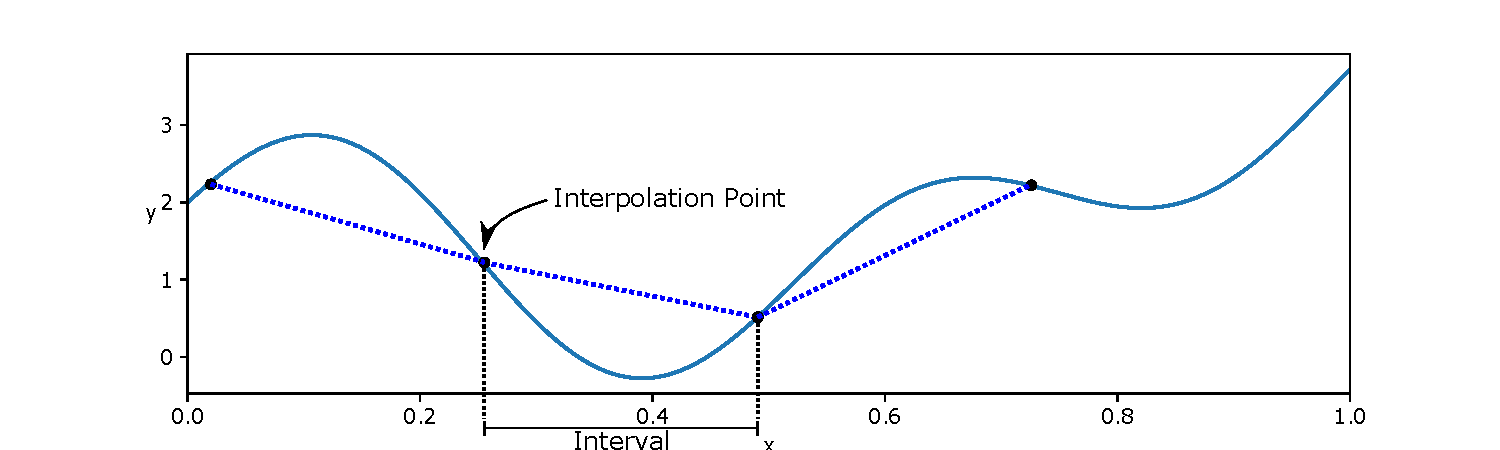
\includegraphics[width=0.90\linewidth]{exponentials/interpolation-example}
          \caption{Example of linear interpolation with uniform interval widths and interpolation points on the edge of the domain.\label{fig:LSMOC:ET:Interpolation Example}}
        \end{figure}

        Let $P_n(x)$ be the order $n$ polynomial approximating a function, $f(x)$, on an arbitrary interval $[a,b]$.
        The maximum error, $\epsilon$, within an interval is given by
        \begin{equation}\label{eq:LSMOC:ET:Interpolation Error}
          \epsilon = \frac{1}{(n+1)!}\left(\max_{\xi\in[a,b]}\lrabs{f^{(n+1)}(\xi)}\right)\left(\max_{x\in[a,b]}\lrabs{\prodl[j=1][n+1](x-x_j)}\right),
        \end{equation}
        for some value $\xi\in[a,b]$, where $f^{(n+1)}$ is the $n+1$-th derivative of $f(x)$.
        The choice of interpolation points will only affect the last term enclosed in parentheses.

        The Chebyshev points \cite{Stewart1996} are a set of values in $[a,b]$ that minimize $\max_{x\in[a,b]}\lrabs{\prodl[j=1][n+1](x-x_j)}$, and are given by
        \begin{equation}\label{eq:LSMOC:ET:Chebyshev Points}
          x_k = \frac{1}{2}\left[(a+b)+(b-1)\cos\left(\frac{2k-1}{2(n+1)}\pi\right)\right], \forall k\in\{1,2,...,n,n+1\}.
        \end{equation}
        By using the Chebyshev points, the maximum interpolation error, $\epsilon$, can be simplified to
        \begin{equation}\label{eq:LSMOC:ET:Chebyshev Interpolation Error}
          \epsilon = \frac{1}{2^n(n+1)!}\left(\frac{b-a}{2}\right)^{n+1}\max_{\xi\in[a,b]}\lrabs{f^{(n+1)}(\xi)}.
        \end{equation}
        Because the Chebyshev points do not include the end-points of the interval, there is additional cost in setting up the interpolation table, but this is negligible to typical \ac{MOC} calculation times.
        An interpolation table using Chebyshev points \emph{reduces error at no run-time cost} compared to a table using evenly spaced points.
        For this reason, Chebyshev points will be assumed for the remainder of this section.
        \Cref{tab:LSMOC:ET:Chebyshev Error} shows maximum errors for $F_1(\opt)$ interpolation for uniformly spaced points and Chebyshev points for an interval width $\Delta=b-a$.
        \begin{table}
          \centering
          \renewcommand{\arraystretch}{1.45}
          \caption{Maximum error in $F_1(\opt)$ for interval width $\Delta$.}
          \label{tab:LSMOC:ET:Chebyshev Error}
          \begin{tabular}{@{}ccc@{}}\toprule
            Polynomial Order & Uniform points   & Chebyshev points\\\midrule
            1                & $\frac{\Delta^2}{8}$           & $\frac{\Delta^2}{16}$\\
            2                & $\frac{\Delta^3}{72\sqrt{3}}$  & $\frac{\Delta^3}{192}$\\
            3                & $\frac{\Delta^4}{1536}$        & $\frac{\Delta^4}{3072}$\\\bottomrule
          \end{tabular}
        \end{table}
      }
      \subsubsection{Interval Width}{\label{sssec:LSMOC:ET:Interval Width}
        The conventional approach for interpolation tables has been to use a constant interval width, $\Delta$, for all intervals in the domain.
        This interval width is then used to control the error of the table.
        \Cref{eq:LSMOC:ET:Interpolation Error} shows that the interval bounds affect the interpolation error through the derivative term.
        The second and higher order derivatives of each of the exponential functions (\cref{eqs:LSMOC:ET:Exponential Functions}) approach zero as $\segopt$ approaches infinity.
        This indicates that the interpolation error typically decreases as the optical thickness increases in the conventional approach.

        However, is is possible to maintain the same maximum error over each interval if a variable interval width, $\Delta_i$, is used, where $i$ indicates the interval index.
        By using a variable interval width, a table can use fewer intervals while maintaining the same maximum error.
        However, since the widths are no longer constant, there is no longer a simple/direct conversion from $\segopt$ to $i$.
        Although there may be better ways, for this work the smallest interval is used to break up the domain into a map which points to the correct interval for that range of values.

        It was found that the use of non-uniform interval widths allowed for significantly fewer total intervals, reducing the memory usage, but incurring overhead for the additional mapping to index.
        \Cref{fig:LSMOC:ET:Memory Analysis} shows the memory usage for a polar-independent interpolation table for $F_1(\segopt)$.
        Using a non-uniform table typically decreases the memory usage by nearly an order of magnitude.
        For polar-dependent tables, the memory usage will be multiplied by the largest inverse sine of the polar angle, and the number of polar angles.

        \begin{figure}
          \centering
          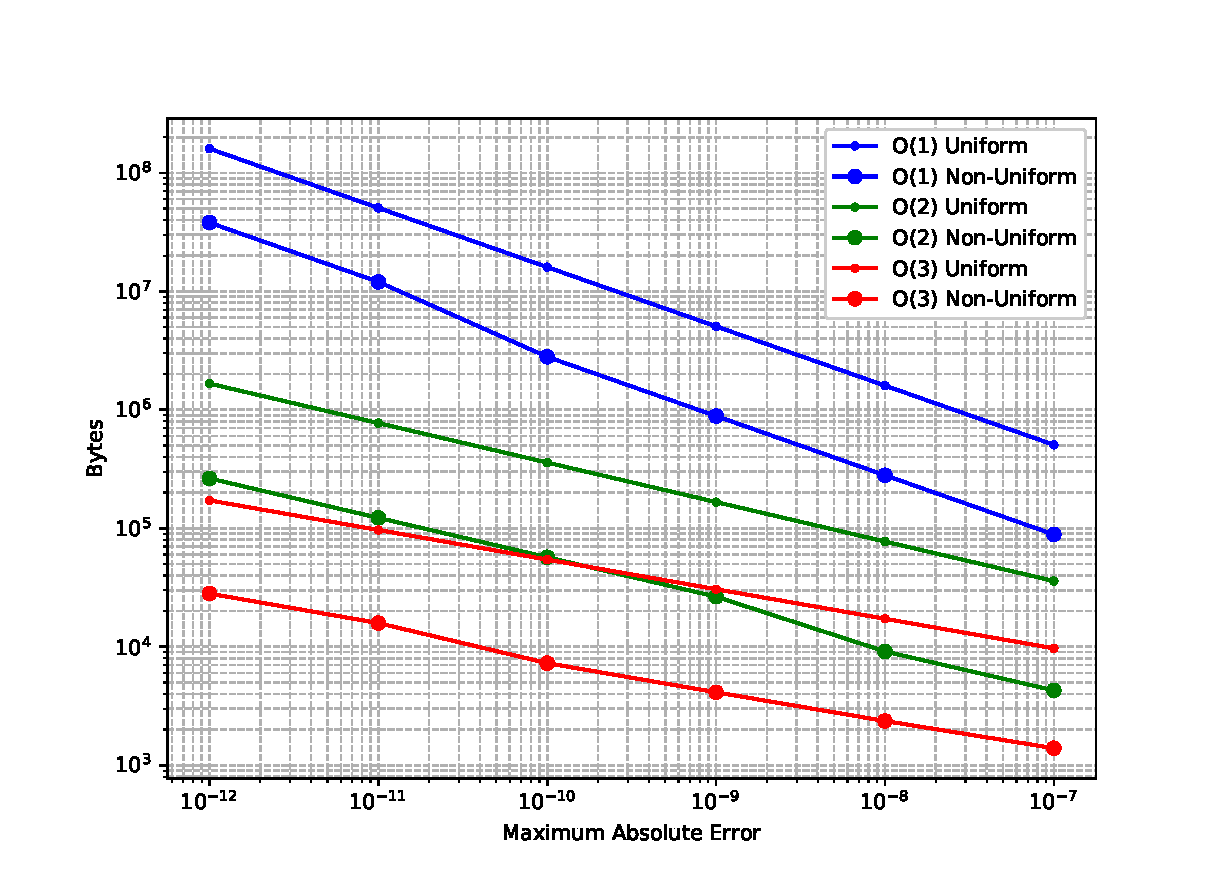
\includegraphics[width=0.90\linewidth]{exponentials/MemoryAnalysis}
          \caption{The memory usage of a single interpolation table (polar independent) for $F_1(\segopt)$ is shown as a function of the maximum error for different interpolation orders and tabulation methods.\label{fig:LSMOC:ET:Memory Analysis}}
        \end{figure}

        Because all the functions of \cref{eq:LSMOC:ET:Exponential Functions} are related, it is possible to tabulate only a single function and compute the others from the resulting interpolated value.
        However, if $F_1(\segopt)$ is known accurately, it is not possible to compute $H(\segopt)$ for very small $\segopt$ due to round-off errors.
        Instead one can tabulate $H(\segopt)$ and use the result to compute the other functions; however, this may incur more error than directly interpolating these functions.
      }
    }
    \subsection{Function Modification}{\label{ssec:LSMOC:ET:Function Modification}
      A second approach for addressing the instability due to inaccurate function interpolation was taken: change the functions.
      Recall that the highly accurate interpolation tables of \cref{ssec:LSMOC:ET:First Approach: Improved Accuracy} were necessary due to the inverse total (or transport) cross section on the $F_2(\segopt)$ term of \cref{eq:LSMOC:ET:Transmission Original}.
      Manipulating this term, we define a new function
      \begin{equation}\label{eq:LSMOC:ET:F2 Modified Definition}
        \frac{F_2(\segopt)}{\xst} = \nlen\modFunc,
      \end{equation}
      where
      \begin{equation}\label{eq:LSMOC:ET:F2 Modified}
        \modFunc \defined 2\left(1-\frac{F_1(\segopt)}{\segopt}\right) - F_1(\segopt).
      \end{equation}
      The $\modFunc$ function can be tabulated in place of $F_2(\segopt)$; this will require an additional multiplication by the segment length $\nsegl$ causing slight reduction in performance.
      But, by using the modified $\modFunc$ function, the underlying cause of the numerical instability is addressed, and the more accurate interpolation is no longer necessary.

      One approach is to tabulate the $\modFunc$ function in place of the $F_2(\segopt)$ function, and multiply by $\nsegl$ during evaluation.
      However, as stated in the previous section, it is possible to tabulate a single function and compute the others.
      The $H(\segopt)$ function could be tabulated again; but tabulating an intermediate function,
      \begin{equation}\label{eq:LSMOC:ET:E1}
        E_1(\segopt) \defined \frac{1-e^{-\segopt}}{\segopt},
      \end{equation}
      uses the same number of operations to compute the other functions.
      This $E_1(\segopt)$ function also has smaller derivative terms around $\segopt=0$, allowing for larger interval widths with no loss in accuracy.
      Therefore, it is expected that $E_1(\segopt)$ tabulation will be more efficient.
    }
    \subsection{Results}{\label{ssec:LSMOC:ET:Results}
      \blindtext[5]
    }
  }
  %%%%%%%%%%%%%%%%%%%%%%%%%%%%%%%%%%%%%%%%%%%%%%%%%%%%%%%%%%%%%%%%%%%%%%%%%%%%%%
  % Improved Linear Source Formulation for Multi-physics and 2D/1D Applications
  %%%%%%%%%%%%%%%%%%%%%%%%%%%%%%%%%%%%%%%%%%%%%%%%%%%%%%%%%%%%%%%%%%%%%%%%%%%%%%
  \section{Improved Linear Source Formulation for Multi-physics and 2D/1D Applications}{\label{sec:Improved Linear Source Formulation for Multi-physics and 2D/1D Applications}
    \blindtext
    \subsection{Derivation}{\label{ssec:LSMOC:Derivation}
      \blindtext[5]
    }
    \subsection{Results}{\label{ssec:LSMOC:Results}
      \blindtext[5]
    }
  }


  % References
  \printbibliography
}


% \subsection{Derivation}{\label{ssec:MOC:LSA:Derivation}
% The moment-based \ac{LSA} assumes the shape of the source, $\source[mi][g][\loc]$, is spatially linear within each cell, $\Region$.
% This can be expressed as
% \begin{subequations}\label{eqs:MOC:LSA:Source Shape}
%     \begin{equation}\label{eq:MOC:LSA:Source Shape}
%         \source[mi][g][\loc] \approx \srcF[mi] + \loc\vdot\srcL,
%     \end{equation}
%     where $\srcL$ is a column vector of source spatial expansion coefficients,
%     \begin{equation}
%         \srcL \defined\begin{bmatrix}\srcL[x]\\\srcL[y]\\\srcL[z]\end{bmatrix},
%     \end{equation}
%     and $\loc$ is the position in \emph{local} coordinates.
% \end{subequations}
% A similar spatial expansion of the angular moments of the flux can be performed,
% \begin{equation}\label{eq:MOC:LSA:Flux Expansion}
%     \fluxA(\loc) = \fluxF + \loc\vdot\fluxL,
% \end{equation}
% the source can then be expressed as
% \begin{equation}\label{eq:MOC:LSA:Linear Source Computation}
%     \source[mi][g][\loc]
%         = \suml[\gprime]\suml[\ell=0][L]\suml[n=-\ell][\ell]\SH[\ell][n][\dirm]\xss[\ell]\fluxA[\gprime](\loc)
%         + \frac{\spect}{\keff}\suml[\gprime]\nufis\sflux[\gprime](\loc),
% \end{equation}
% and the linear expansion coefficients are explicitly given by
% \begin{equation}\label{eq:MOC:LSA:Linear Source Coefficients}
%     \srcL
%         = \suml[\gprime]\suml[\ell=0][L]\suml[n=-\ell][\ell]\SH[\ell][n][\dirm]\xss[\ell]\fluxL[\gprime]
%         + \frac{\spect}{\keff}\suml[\gprime]\nufis\sfluxL[\gprime].
% \end{equation}

% In the spatial moment-base \ac{LSA}, it is convenient to define the spatially linear source (and flux) in terms of a cell-local coordinate system.
% Allow $\Loc$ to be the position variable in the global coordinate system, the local coordinates are then defined as
% \begin{equation}\label{eq:MOC:LSA:Global to Local Coordinates}
%     \loc = \Loc - \centroid[\Loc][mi],
% \end{equation}
% where $\centroid[\Loc][mi]$ is the numerical centroid of the cell $i$.

% These numerical centroids can be defined as either direction-dependent, or direction-independent, which will have implications on particle conservation, as discussed in \cref{ssec:MOC:LSA:Particle Conservation}.
% The direction-dependent centroids are defined by
% \begin{equation}\label{eq:MOC:LSA:Direction-Dependent Centroids}
%     \centroid[\Loc][mi] \defined \MOCSingleAngleIntegral{\Loc} = \frac{1}{V_i}\suml[k]\tA[mki]\nsegl\locCent[\Loc],
% \end{equation}
% where $\locCent[\Loc]$ is the global coordinate vector of the track-segment mid-point.
% Similarly, the direction-independent centroids are defined by
% \begin{equation}\label{eq:MOC:LSA:Direction-Independent Centroids}
%     \centroid[\Loc][i] \defined \rfourpi\MOCIntegral{\Loc} = \frac{1}{V_i}\suml[m]\wt\suml[k]\tA[mki]\nsegl\locCent[\Loc].
% \end{equation}

% Following the same approach as the \ac{FSMOC} derivation, in \cref{ssec:MOC:FSA:Derivation}, computing the source the region-averaged flux moment, $\fluxF$, and the flux expansion coefficients, $\fluxL$, are required.
% \begin{subequations}\label{eqs:MOC:LSA:Region-Averaged Flux Moments Definitions}
%     The region-averaged flux moment can be found using the same definition as previously,
%     \begin{equation}\label{eq:MOC:LSA:Region-Averaged Flux Moment Definition}
%         \fluxF \defined \MOCIntegral{\SH \aflux[][g][]} = \frac{\fourpi}{V_i}\suml[m]\wt\SH[\ell][n][\dirm]\suml[k]\tA[mki]\nsegl\MOCTrackIntegral{\aflux[][g][]}.
%     \end{equation}
%     In order to determine the spatial expansion coefficients of the flux moments, \cref{eq:MOC:LSA:Flux Expansion} is operated on by $\MOCIntegral{\SH(\vdot)\loc^T}$.
%     Recognizing that this should be directly proportional to angular flux operated on by $\MOCIntegral{\SH\aflux[][g][]\loc^T}$, a system of equations is found
%     \begin{equation}\label{eq:MOC:LSA:Moment to Expansion Coefficient}
%         \M\fluxL = \MOCIntegral{\SH\loc\aflux[][g][]},
%     \end{equation}
%     where
%     \begin{equation}\label{eq:MOC:LSA:Geometric Moments}
%         \M \defined \MOCIntegral{\loc^T\loc}.
%     \end{equation}
%     The spatial angular flux moments, $\MOCIntegral{\SH\loc\aflux[][g][]}$, are then defined as
%     \begin{equation}\label{eq:MOC:LSA:Revion-Averaged Spatial Angular Flux Moments Definition}
%         \MOCIntegral{\SH\loc\aflux[][g][]} = \frac{\fourpi}{V_i}\suml[m]\wt\SH[\ell][n][\dirm]\suml[k]\tA[mki]\nsegl\left(\locIn\MOCTrackIntegral{\aflux[][g][]} + \dirm\MOCTrackIntegral{\nlen\aflux[][g][]} / \renorm[mi]\right).
%     \end{equation}
% \end{subequations}

% In order to evaluate the flux moments defined in \cref{eqs:MOC:LSA:Region-Averaged Flux Moments Definitions}, the track-averaged angular flux values, $\MOCTrackIntegral{\aflux[][g][]}$, and $\MOCTrackIntegral{\nlen\aflux[][g][]}$, must be determined.
% First, the transport equation must be put into characteristic form, using \cref{eq:MOC:Renormalized Location Variable} the spatially expanded source, \cref{eq:MOC:LSA:Source Shape}, can be defined along the characteristic.
% \begin{subequations}\label{eqs:MOC:LSA:Characteristic Form}
%     The characteristic transport equation becomes
%     \begin{equation}\label{eq:MOC:LSA:Characteristic Form}
%         \left[\deriv{}{\nlen} + \xst\right]\aflux = \tsrcF + \tsrcL\left(\nlen - \frac{\nsegl}{2}\right),
%     \end{equation}
%     where
%     \begin{equation}\label{eq:MOC:LSA:Track Average Source}
%         \tsrcF \defined \rfourpi\left[\srcF[mi] + \locCent \vdot \srcL\right],
%     \end{equation}
%     and
%     \begin{equation}\label{eq:MOC:LSA:Track Linear Source}
%         \tsrcL \defined \rfourpi\left[\frac{\dirm\vdot\srcL}{\renorm[mi]}\right].
%     \end{equation}
% \end{subequations}
% This can be solved analytically for the angular flux along the track,
% \begin{subequations}\label{eqs:MOC:LSA:Angular Flux Solution}
%     \begin{equation}\label{eq:MOC:LSA:Angular Flux Solution}
%         \aflux = \afluxin + \left(\frac{\tsrcF}{\xst} - \afluxin\right)F_1(\opt) + \frac{\tsrcL}{2(\xst)^2}F_2(\opt),
%     \end{equation}
%     where
%     \begin{equation}\label{eq:MOC:LSA:F1}
%         F_1(\opt) \defined 1 - \exp(-\opt),
%     \end{equation}
%     and
%     \begin{equation}\label{eq:MOC:LSA:F2}
%         F_2(\opt) \defined 2[\opt-F_1(\opt)] - \segopt F_1(\opt).
%     \end{equation}
% \end{subequations}

% As discussed in \cref{ssec:MOC:FSA:Derivation}, there are two \emph{equivalent} methods with which one could determine the track-averaged angular flux values.
% However, it is the author's opinion that defining these moments implicitly, by taking the moments of the characteristic equation (\cref{eq:MOC:LSA:Characteristic Form}), results in a form that is simpler.
% The original basis of this work \cite{Ferrer2016}, evaluated the linear moment explicitly; for brevity, the derivation will only be shown here with the implicitly defined moment.
% Previous work \cite{Fitzgerald2019} has also shown that by using the form given by the implicit definition, there are significant benefits in multi-physics applications.
% The implicitly defined moments, given by operating on \cref{eq:MOC:LSA:Characteristic Form} by $\MOCTrackIntegral{(\vdot)}$ and $\MOCTrackIntegral{\nlen(\vdot)}$, are given by
% \begin{subequations}\label{eqs:MOC:LSA:Track-Averaged Moments}
%     \begin{equation}\label{eq:MOC:LSA:Track-Averaged Angular Flux}
%         \MOCTrackIntegral{\aflux[][g][]} = \frac{\tsrcF}{\xst} + \frac{\dflux}{\segopt},
%     \end{equation}
%     and
%     \begin{equation}\label{eq:MOC:LSA:Track-Averaged Linear Angular Flux}
%         \MOCTrackIntegral{\nlen\aflux[][g][]} = \frac{\MOCTrackIntegral{\aflux[][g][]} - \afluxout}{\xst} + \frac{\nsegl}{2}\left[\frac{\tsrcF}{\xst} + \frac{\tsrcL}{\xst}\frac{\nsegl}{6}\right].
%     \end{equation}
% \end{subequations}
% Due to the presence of the $\dflux/\segopt$ term in \cref{eq:MOC:LSA:Track-Averaged Linear Angular Flux}, it is beneficial to stability and performance \cite{Fitzgerald2018,Fitzgerald2019} to compute this quantity directly, rather than computing $\dflux$ (as is done for \ac{FSMOC}).
% \begin{subequations}\label{eqs:MOC:LSA:Delta Flux over Optical Thickness}
%     This can be found explicitly by subtracting \cref{eq:MOC:LSA:Angular Flux Solution} evaluated at the exiting location from $\afluxin$ and dividing by $\segopt$, to get
%     \begin{equation}\label{eq:MOC:LSA:Delta Flux over Optical Thickness}
%         \frac{\dflux}{\segopt} = \left(\afluxin-\frac{\tsrcF}{\xst}\right)E_1(\segopt) - \frac{\nsegl}{2}\frac{\tsrcL}{\xst}T_2(\segopt),
%     \end{equation}
%     where
%     \begin{equation}\label{eq:MOC:LSA:E1}
%         E_1(\segopt) \defined \frac{F_1(\segopt)}{\segopt},
%     \end{equation}
%     \begin{equation}\label{eq:MOC:LSA:T2}
%         T_2(\segopt) \defined 2E_2(\segopt) - E_1(\segopt),
%     \end{equation}
%     and
%     \begin{equation}\label{eq:MOC:LSA:E2}
%         E_2(\segopt) \defined \frac{1-E_1(\segopt)}{\segopt}.
%     \end{equation}
% \end{subequations}
% }
% \subsection{Particle Conservation}{\label{ssec:MOC:LSA:Particle Conservation}
% In consideration to particle balance, use of the \ac{LSA} results in additional constraints on the calculations.
% Similarly to \cref{ssec:MOC:FSA:Particle Conservation}, the track-based integration of the source must exactly integrate to the spatial and angular moments of the source.
% The conservation of spatial moments is the basis of this \ac{LSA} \cite{Ferrer2018}, so this constraint is satisfied without additional constraints on the method.
% The angular moment constraint is expressed as
% \begin{equation}\label{eq:MOC:LSA:Angular Moment Constaint}
%     \rfourpi\MOCIntegral{\SH\source[mi][g][\loc]} = \srcF[i,\ell][g,n].
% \end{equation}
% In addition to the constraints introduced in \cref{ssec:MOC:FSA:Particle Conservation}, namely direction-dependent renormalization, and directional quadrature restrictions, this places constraints on the definition of the local coordinate system:
% \begin{equation}\label{eq:MOC:LSA:Anisotropic Coordinate Constraint}
%     \MOCSingleAngleIntegral{\loc} = 0.
% \end{equation}
% This is equivalent to stating that the local coordinate system must be defined with respect to direction-dependent global centroids, as is given by \cref{eq:MOC:LSA:Direction-Dependent Centroids}.

% If these constraints are satisfied, \cref{eqs:MOC:LSA:Region-Averaged Flux Moments Definitions} can be simplified,
% \begin{subequations}\label{eqs:MOC:LSA:Region-Averaged Flux Moments}
%     \begin{equation}\label{eq:MOC:LSA:Region-Averaged Scalar Flux}
%         \sflux = \frac{\srcF}{\xst} + \frac{\fourpi}{V_i\xst}\suml[m]\wt[m]\suml[k]\tA[mki]\dflux,
%     \end{equation}
%     \begin{equation}\label{eq:MOC:LSA:Region-Averaged Angular Moments of Flux}
%         \fluxF = \frac{\tsrcF[i,\ell][g,n]}{\xst} + \frac{\fourpi}{V_i\xst}\suml[m]\wt[m]\SH[\ell][n][\dirm]\suml[k]\tA[mki]\dflux,
%     \end{equation}
%     and
%     \begin{aequation}\label{eq:MOC:LSA:Region-Averaged Spatial Moments of Flux}
%         \MOCIntegral{\loc\SH\aflux[][g][]}
%             &= \suml[m]\wt\SH[\ell][n][\dirm]\M[][mi]\frac{\srcL[][mi]}{\xst}\\
%             &+ \frac{\fourpi}{V_i\xst}\suml[m]\wt\SH[\ell][n][\dirm]\suml[k]
%                 \tA\left[\locIn\dflux + \dirm\segl\left(\frac{\dflux}{\segopt}-\afluxout + \frac{\tsrcF}{\xst}\right)\right]
%     \end{aequation}
%     where
%     \begin{equation}\label{eq:MOC:LSA:Delta Flux}
%         \dflux \defined \afluxin - \afluxout,
%     \end{equation}
%     and
%     \begin{equation}\label{eq:MOC:LSA:Direction Dependent M}
%       \M[][mi] \defined \MOCSingleAngleIntegral{\loc^T\loc}.
%     \end{equation}
% \end{subequations}
% }
% \subsection{Spatial and Isotropic Simplifications}{\label{ssec:MOC:LSA:Isotropic Simplifications}
% The work introducing the original formulation of the moment-based \ac{LSA} suggests that it is beneficial to allow only the isotropic moments of the source and flux to be spatially linear, while higher order moments are spatially flat.
% The reformulation introduced as part of this work \cite{Fitzgerald2019} was extended to make this simplification in the so called \acf{LIFA} source [CITATION].
% The linear moment equations can then be simplified to
% \begin{aequation}\label{eq:MOC:LSA:LIFA Region-Averaged Spatial Moments of Flux}
%     \MOCIntegral{\loc\aflux[][g][]}
%         &= \M\frac{\srcL}{\xst}
%         + \frac{\fourpi}{V_i\xst}\suml[m]\wt\suml[k]
%             \tA\left[\locIn\dflux + \dirm\segl\left(\frac{\dflux}{\segopt} - \afluxout + \frac{\tsrcF}{\xst}\right)\right].
% \end{aequation}

% In the case of an isotropic source, the constraints for particle balance are relaxed.
% Track-length renormalization as well as numerical centroid definitions can be direction-independent while still preserving particle conservation \cite{Ferrer2018}, as given by \cref{eq:MOC:Region Renormalization}, and \cref{eq:MOC:LSA:Direction-Independent Centroids} respectively.
% The calculation of angular flux spatial moments, given in \cref{eq:MOC:LSA:Region-Averaged Spatial Moments of Flux}, can also be simplified into the form
% \begin{equation}\label{eq:MOC:LSA:Region-Averaged Spatial Moments of Flux Isotropic}
%     \MOCIntegral{\loc\aflux[][g][]}
%             = \M\frac{\srcL}{\xst}
%             + \frac{\fourpi}{V_i\xst}\suml[m]\wt\suml[k]\tA
%                 \left(\dirm\segl\left[\frac{\dflux}{\segopt} - \afluxout\right]+ \locIn\dflux\right).
% \end{equation}
% }
    \chapter{Initial Results}{\label{ch:Initial Results}
    \def\figpath{chapters/06/figures/}
    \graphicspath{ {\figpath} }

    \section{2-D Linear Source}{\label{sec:Results:2-D Linear Source}
        The \ac{LSMOC} method has been a significant part of this thesis work.
        The method, as described by \citet{Ferrer2016}, was implemented in MPACT \cite{Collins2016}, and has been significantly improved for cases with near-void regions \cite{Fitzgerald2018}, and multiphysics calculations \cite{Fitzgerald2019}.
        So far, detailed analysis has only been done for 2-D calculations; in this section, the results from a conference paper on the improved formulation are presented.
        Work done by others has indicated that for single physics (neutronics) calculations, significantly coarser meshes can be used with the \ac{LSA} as compared to the \ac{FSA} \cite{Ferrer2016,Boyd2014,Gunow2018}, resulting in faster computations; the goal of this conference paper was to present a reformulation of the method, that is more efficient in multi-physics calculations, as well as present results to indicate that coarser meshes could still be used \cite{Fitzgerald2019}.
        At the current time, all results are presented using \ac{TCP0} cross sections and odCMFD acceleration \cite{Zhu2016}.

        In this work, two additional physics are considered: isotopic depletion, and \ac{TH} feedback.
        Typical \acp{LWR} use \acs{UO2} fuel; however, a significant fraction of power comes from plutonium fission events.
        As a fuel rod is depleted during reactor operation, plutonium builds up in the outer rim of the fuel rods.
        In calculations with isotopic depletion, it is necessary to accurately capture this radial distribution of plutonium.
        In MPACT-CTF coupling, fuel temperatures are averaged radially.
        Since there is no radial dependence, it is not necessary to consider additional radial meshing to account for this physics.
        However, there is current work to add radially dependence to \ac{TH} feedback quantities in the coupling between MPACT and CTF, and this is common in other high fidelity neutronics codes.
        This may affect the number of rings needed in fuel meshes, for both the \ac{FSMOC} and \ac{LSMOC} solvers.

        To help determine optimal default meshing parameters for the \ac{LSMOC} solver in MPACT, a parametric study was done on a pin cell with isotopic depletion up to 70 MWD/kgHM.
        Using the default \ac{FSMOC} mesh as a starting point, the meshing parameters were coarsened; for each parameter, the coarsest option, that did not cause significant change in the eigenvalue over the depletion, was selected.
        The resulting coarse mesh has two fuel rings (inner radius at 87.5\% of outer), a single ring in the cladding, a single ring in the gap, and four azimuthal divisions in all regions.
        However, in the lattice and assembly test cases, a single azimuthal region was found to be sufficient in the fuel, clad, and gap material regions when using the \ac{LSMOC} solver.
        The inner fuel radius at 87.5\% of the outer radius is consistent with measured radial distributions of plutonium in irradiated \acs{UO2} fuel rods \cite{Lassmann1994}.
        This mesh, along with the default \ac{FSMOC} mesh, is shown in \cref{fig:Results:LSA:Depletion:Meshes}.

        Results from three cases are presented in the following subsections: 2D zero-power lattice cases, 2D lattice depletion cases, and a 3D fuel assembly with \ac{TH} feedback.

        \subsection{Pin Cell Isotopic Depletion}{\label{ssec:Results:LSA:Pin Cell}
            As reactors operate, interactions of the fuel with neutrons causes isotopic changes within the fuel, over long periods this can lead to significant changes in the fuel composition.
            Changes in the fuel composition play an important role in the power distribution as a reactor operates, and is thus a key additional physics to consider in reactor simulations.
            A parametric mesh-refinement study are presented for a single \acs{UO2} pin cell depletion up to 70 MWD/kgHM.

            During depletion, it is important to accurately capture the radial distribution of Plutonium due to self-shielding effects.
            However, Plutonium is primarily concentrated in the outer rim of the pin, this is the well known rim-effect.
            The expectation is that a single additional fuel ring can be used to capture this rim effect.
            This was found to be the case, with an inner ring with radius fraction 0.875 that of the outer fuel radius \cite{Fitzgerald2019}.
            This seems to be consistent with measured radial Plutonium distributions \cite{Lassmann1994}.
        }
        \subsection{2-D Zero-Power Lattice Cases}{\label{ssec:Results:LSA:2-D Zero-Power Lattice Cases}
            Initial tests were run on a series of zero-power 2-D lattices: the \ac{VERA} problem 2 cases \cite{VERAProblems}.
            By doing so, it can be verified that the \ac{LSMOC} solvers are as accurate on this coarse mesh as the \ac{FSMOC} solver on the current default mesh parameters in MPACT.
            These cases cover a variety of lattice configurations as different temperatures, with and without burnable absorbers or other inserts.
            Each case is described in detail in the reference \cite{VERAProblems}.

            Each lattice case was run with default and coarse meshes with the \ac{FSMOC} and \ac{LSMOC} solvers.
            Each of these cases used a Tabuchi-Yamamoto angular quadrature set \cite{TabuchiYamamotoQuad} with 64 azimuthal angles, 4 polar angles over 4$\pi$, and 0.05 cm ray-spacing.
            However, due to thin regions from IFBA and WABA rods in cases L, M, and N, a ray-spacing of 0.01 cm was used.
            The results are compared against a very finely meshed case run using the \ac{LSMOC} solver with 128 azimuthal angles, 4 polar angles, and 0.01 cm ray-spacing.
            Results are summarized in \cref{tab:Results:LSA:Zero Power Lattice Results}.

            On average, the \ac{LSMOC} solver on the coarse mesh is more accurate than the \ac{FSMOC} solver on the current default mesh.
            Additionally, the largest differences for both eigenvalue and RMS pin power differences are smaller than those for the \ac{FSMOC} solver.
            This indicates that, for these cases, the \ac{LSMOC} solver on the coarse mesh is sufficiently accurate.
            On average, the \ac{LSMOC} solver on the coarse mesh took 12\% less time per iteration, and used approximately 12\% less memory.

            \begin{table}[h]
                \centering
                \caption{Results for 2D zero-power lattice cases in terms of eigenvalue difference and RMS pin power difference from the very finely meshed \ac{LSMOC} solution.}
                \label{tab:Results:LSA:Zero Power Lattice Results}
                \begin{tabular}{rrrr@{\hskip 1cm}rrr}
                    \toprule
                    Case    & \multicolumn{3}{c}{$\Delta k_{\text{eff}}$ (pcm)} & \multicolumn{3}{c}{RMS Pin Power Difference (\%)}\\\midrule
                            & FS default   & FS coarse & LS coarse &  FS default   & FS coarse & LS coarse\\\midrule
                          A &    -17.37 &     43.98 &    -36.00 &      0.04 &      0.12 &      0.02\\
                          B &    -14.88 &     46.21 &    -33.83 &      0.04 &      0.12 &      0.02\\
                          C &    -17.37 &     43.98 &    -36.00 &      0.04 &      0.12 &      0.02\\
                          D &    -25.47 &     38.95 &    -40.97 &      0.04 &      0.12 &      0.02\\
                          E &    -49.02 &    -51.80 &    -26.93 &      0.06 &      0.18 &      0.02\\
                          F &    -74.17 &   -119.73 &    -25.68 &      0.05 &      0.18 &      0.02\\
                          G &    -98.35 &   -210.38 &    -42.52 &      0.08 &      0.26 &      0.04\\
                          H &    -77.90 &   -206.12 &     18.40 &      0.11 &      0.32 &      0.07\\
                          I &      2.36 &     82.42 &    -23.56 &      0.04 &      0.14 &      0.03\\
                          J &    -74.18 &   -119.45 &    -25.86 &      0.05 &      0.17 &      0.02\\
                          K &    -61.48 &    -97.41 &    -18.86 &      0.05 &      0.19 &      0.03\\
                          L &     60.38 &    104.64 &     52.02 &      0.06 &      0.17 &      0.05\\
                          M &     74.48 &    123.69 &     71.36 &      0.05 &      0.12 &      0.05\\
                          N &     -0.96 &    -44.92 &     42.85 &      0.11 &      0.32 &      0.04\\
                          O &    -21.26 &   -109.47 &      7.11 &      0.06 &      0.20 &      0.03\\
                          P &   -115.03 &   -311.33 &    -64.06 &      0.09 &      0.28 &      0.05\\
                          Q &    -12.26 &     53.68 &    -30.41 &      0.04 &      0.13 &      0.03\\\midrule
                        Avg. &     46.88 &    106.36 &     35.08 &      0.06 &      0.18 &      0.03\\
                        Max. &    115.03 &    311.33 &     71.36 &      0.11 &      0.32 &      0.07\\\bottomrule
                \end{tabular}
            \end{table}
        }
        \subsection{2-D Lattice Depletion}{\label{ssec:Results:LSA:2-D Lattice Depletion}
            In \cref{ssec:Results:LSA:2-D Zero-Power Lattice Cases}, the \ac{LSMOC} on the coarse mesh was shown to be sufficiently accurate for an array of lattice problems at zero-power.
            Two of these problems, 2a and 2p, were selected for further study by performing isotopic depletion up to 70 MWD/kgHM at HFP conditions.
            Problem 2A represents a typical lattice configuration consisting only of fuel rods and empty guide-tubes.
            Problem 2P contains several gadolinia rods that act as burnable absorbers; reactivity is significantly damped at beginning of cycle, but increases as gadolinia is burned.
            The gadolinia rods require significant radial meshing to accurately capture the complicated distribution throughout the depletion (it is an effectively a \emph{moving boundary layer}); the default meshing for the \ac{FSMOC} solver has 10 equal volume rings in the fuel.
            Due to this complicated distribution, the \ac{LSMOC} solver can only eliminate two of the additional radial rings while maintaining the same level of accuracy as the \ac{FSMOC} solver on the current default mesh.
            However, similar azimuthal coarsening is possible on these rods, with a single azimuthal region in all but the surrounding moderator, which has 4 azimuthal regions.
            Overall, a significant reduction in the lattice mesh is still possible, as shown in \cref{fig:Results:LSA:Depletion:Meshes}.

            As shown in \cref{fig:Results:LSA:Lattice Depletion Results}, the \ac{LSMOC} solver on a coarse mesh has similar accuracy as the \ac{FSMOC} solver on the current default mesh.
            However, the coarse mesh \ac{LSMOC} calculation took took 23\% and 18\% less time for cases A and P, respectively, than the corresponding default mesh \ac{FSMOC} calculations.
            Although the \ac{LSMOC} method was intended, primarily, to increase efficiency in the \ac{MOC} calculation, much of the time saved is actually from reduced time in the isotopic depletion routines.
            21\% and 18\% less memory was used by MPACT in cases A and P, respectively.
            \begin{figure}[h]
                \centering
                \begin{minipage}{0.25\linewidth}
                    \centering
                    \begin{subfigure}[t]{\linewidth}
                        \centering
                        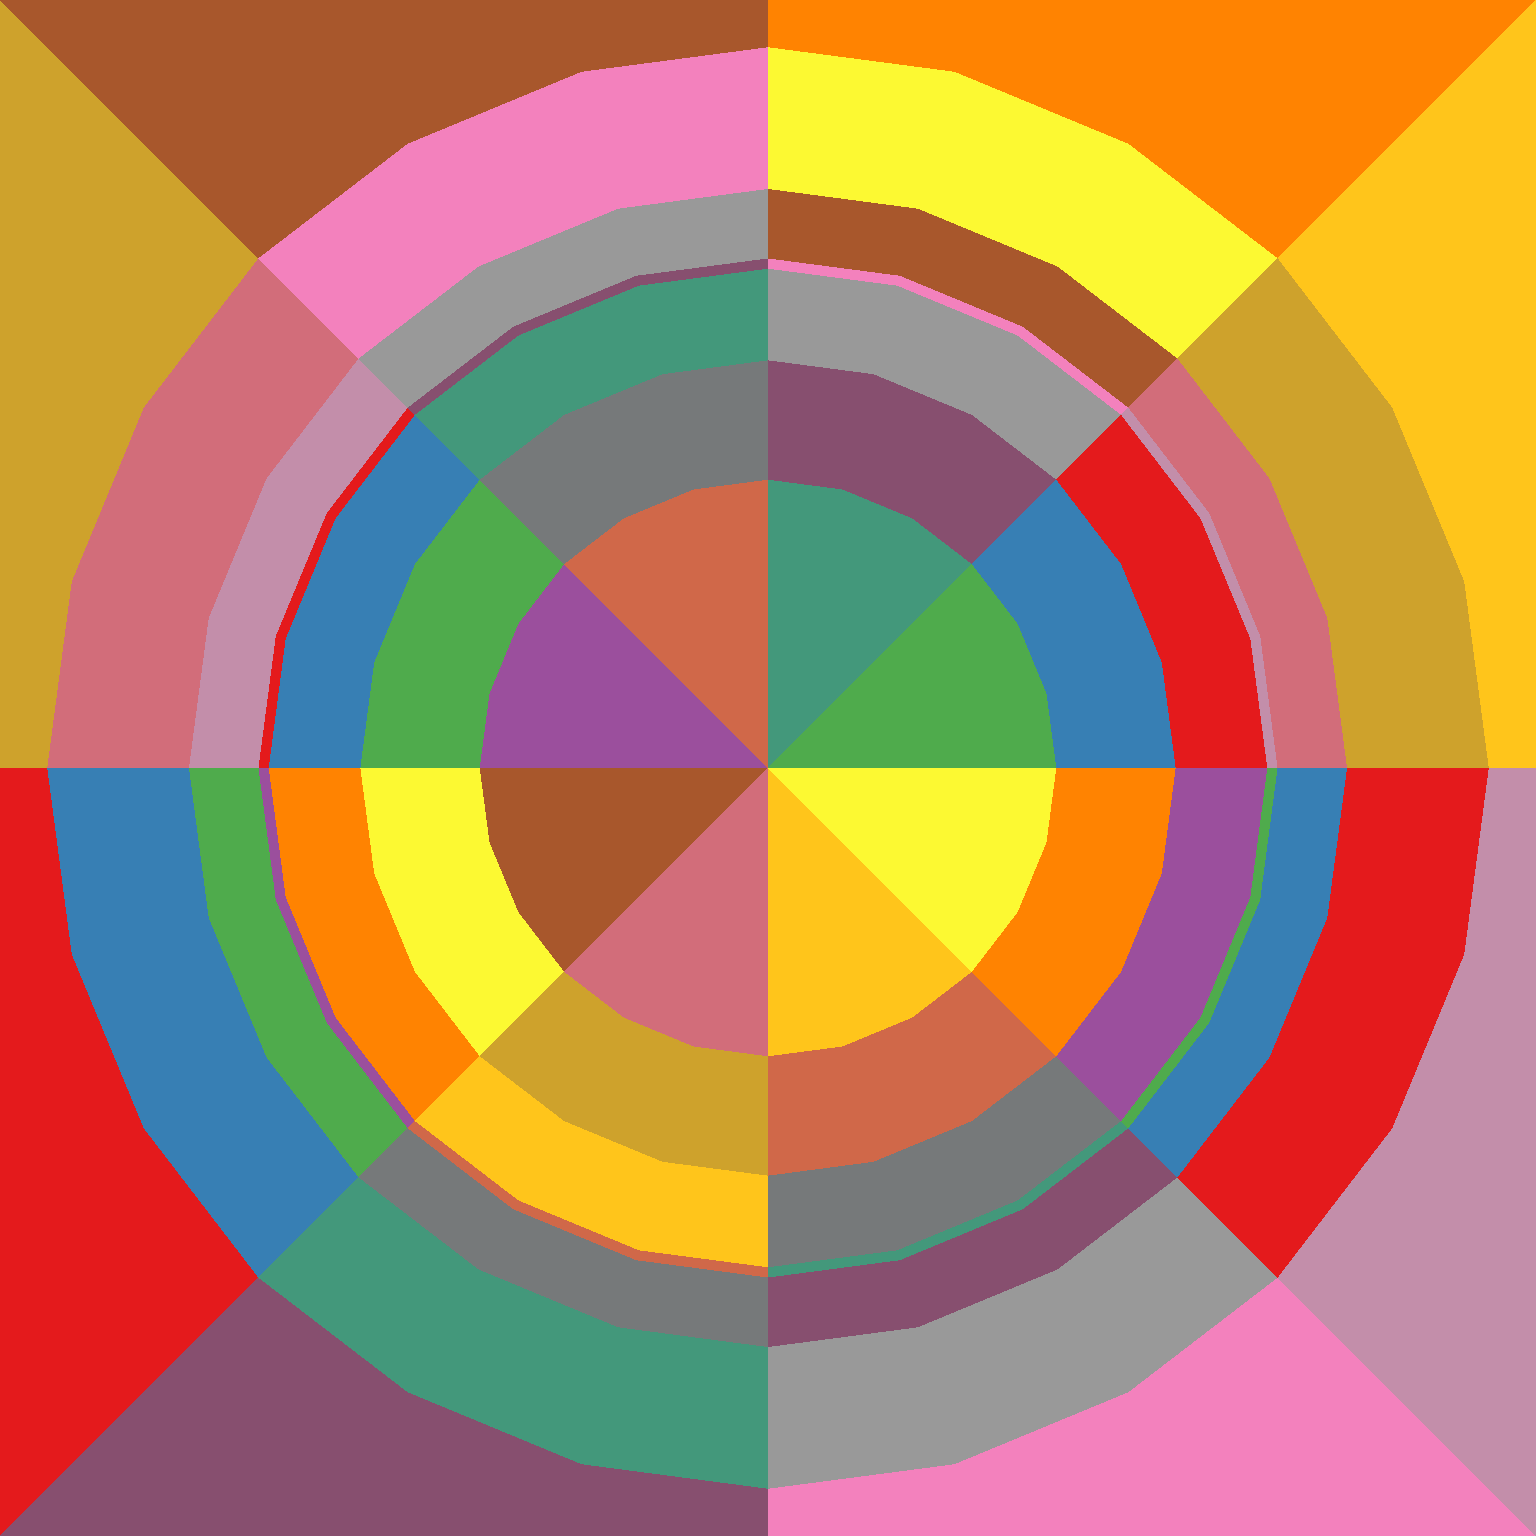
\includegraphics[width=0.45\linewidth]{\figpath/pin/pin-default.png}
                        \caption{Default fuel rod mesh\\\centering(56 cells)}
                    \end{subfigure}
                    \begin{subfigure}[t]{\linewidth}
                        \centering
                        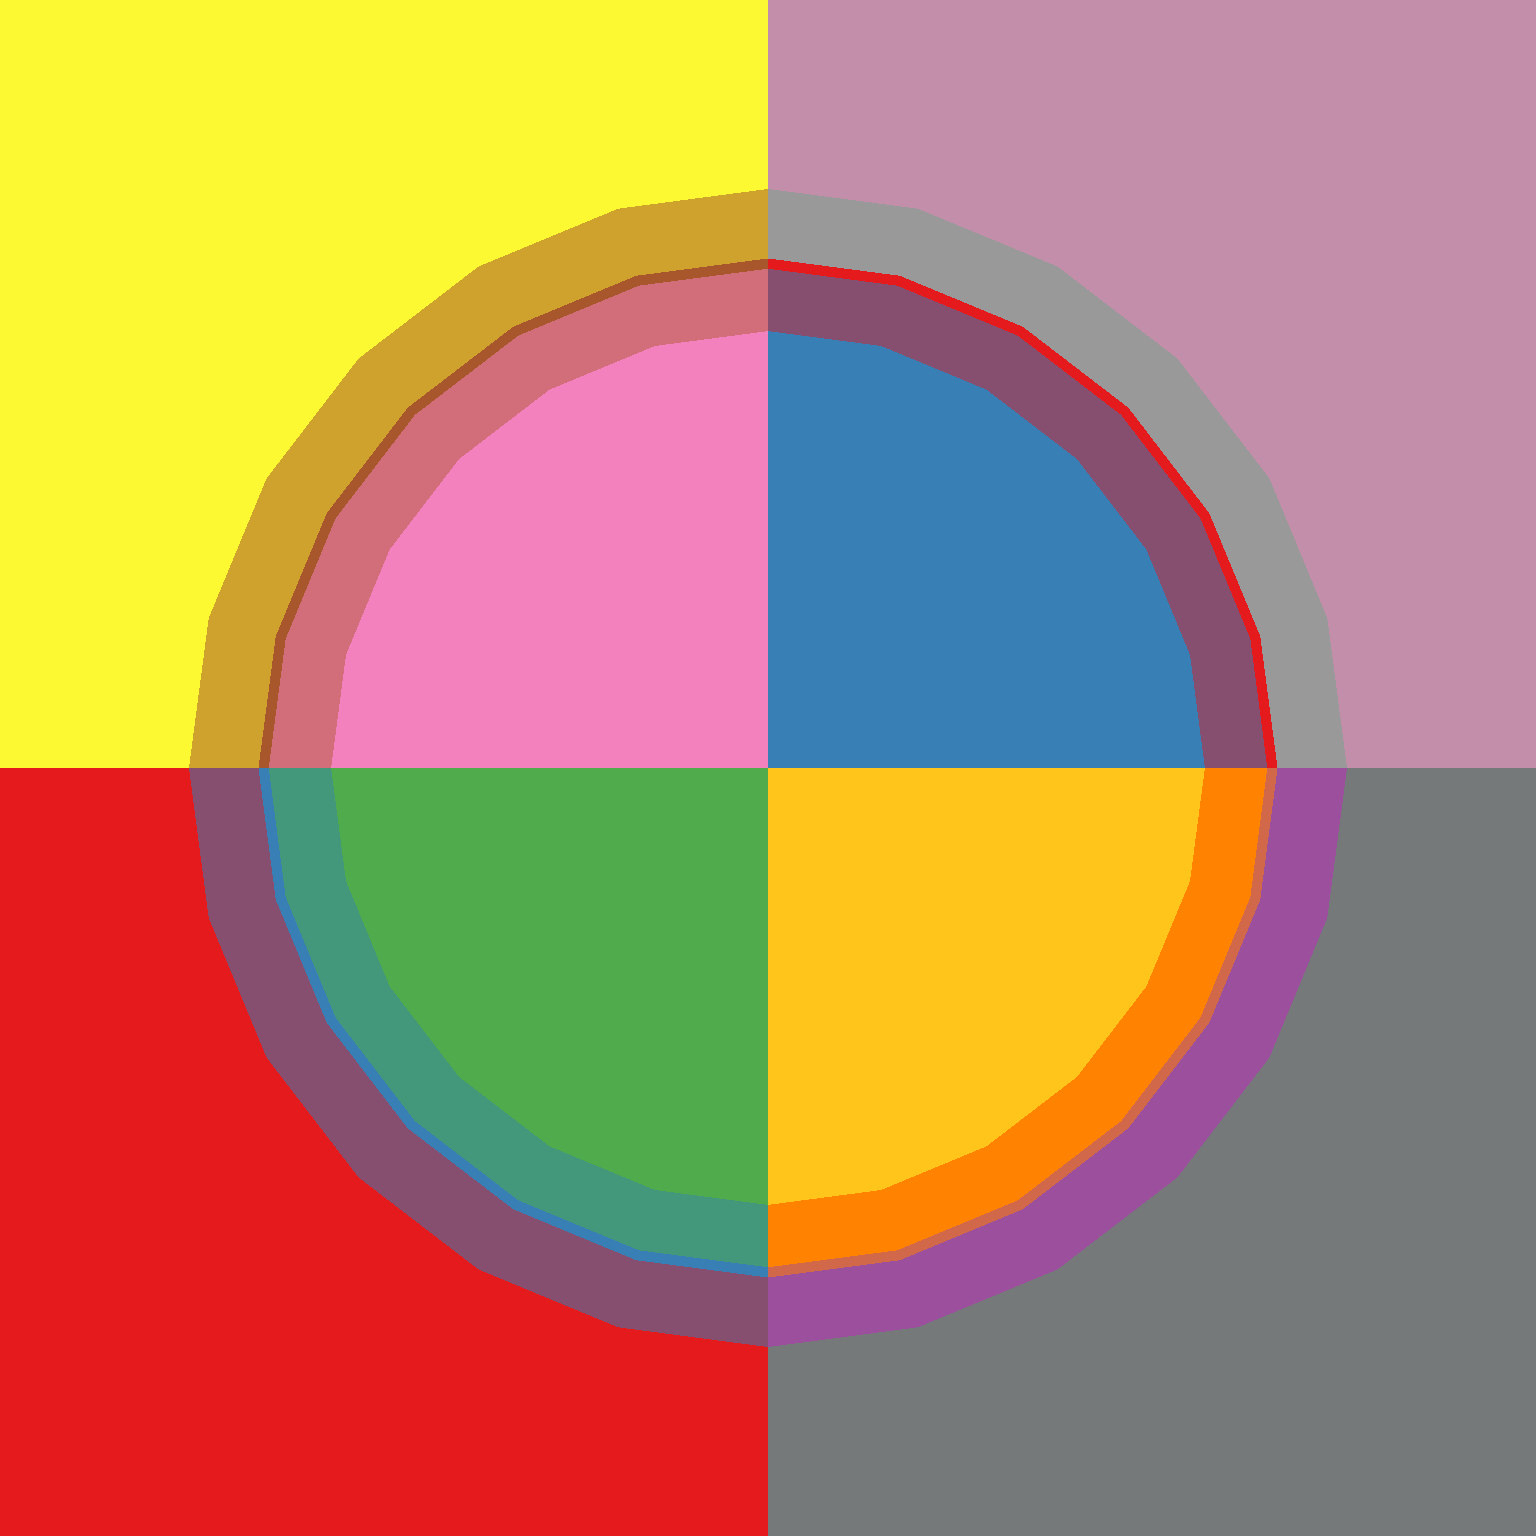
\includegraphics[width=0.45\linewidth]{\figpath/pin/pin-coarse.png}
                        \caption{Coarse fuel rod mesh\\\centering(20 cells)}
                    \end{subfigure}
                \end{minipage}%
                ~
                \begin{minipage}{0.75\linewidth}
                    \centering
                    \begin{subfigure}[t]{0.40\linewidth}
                        \centering
                        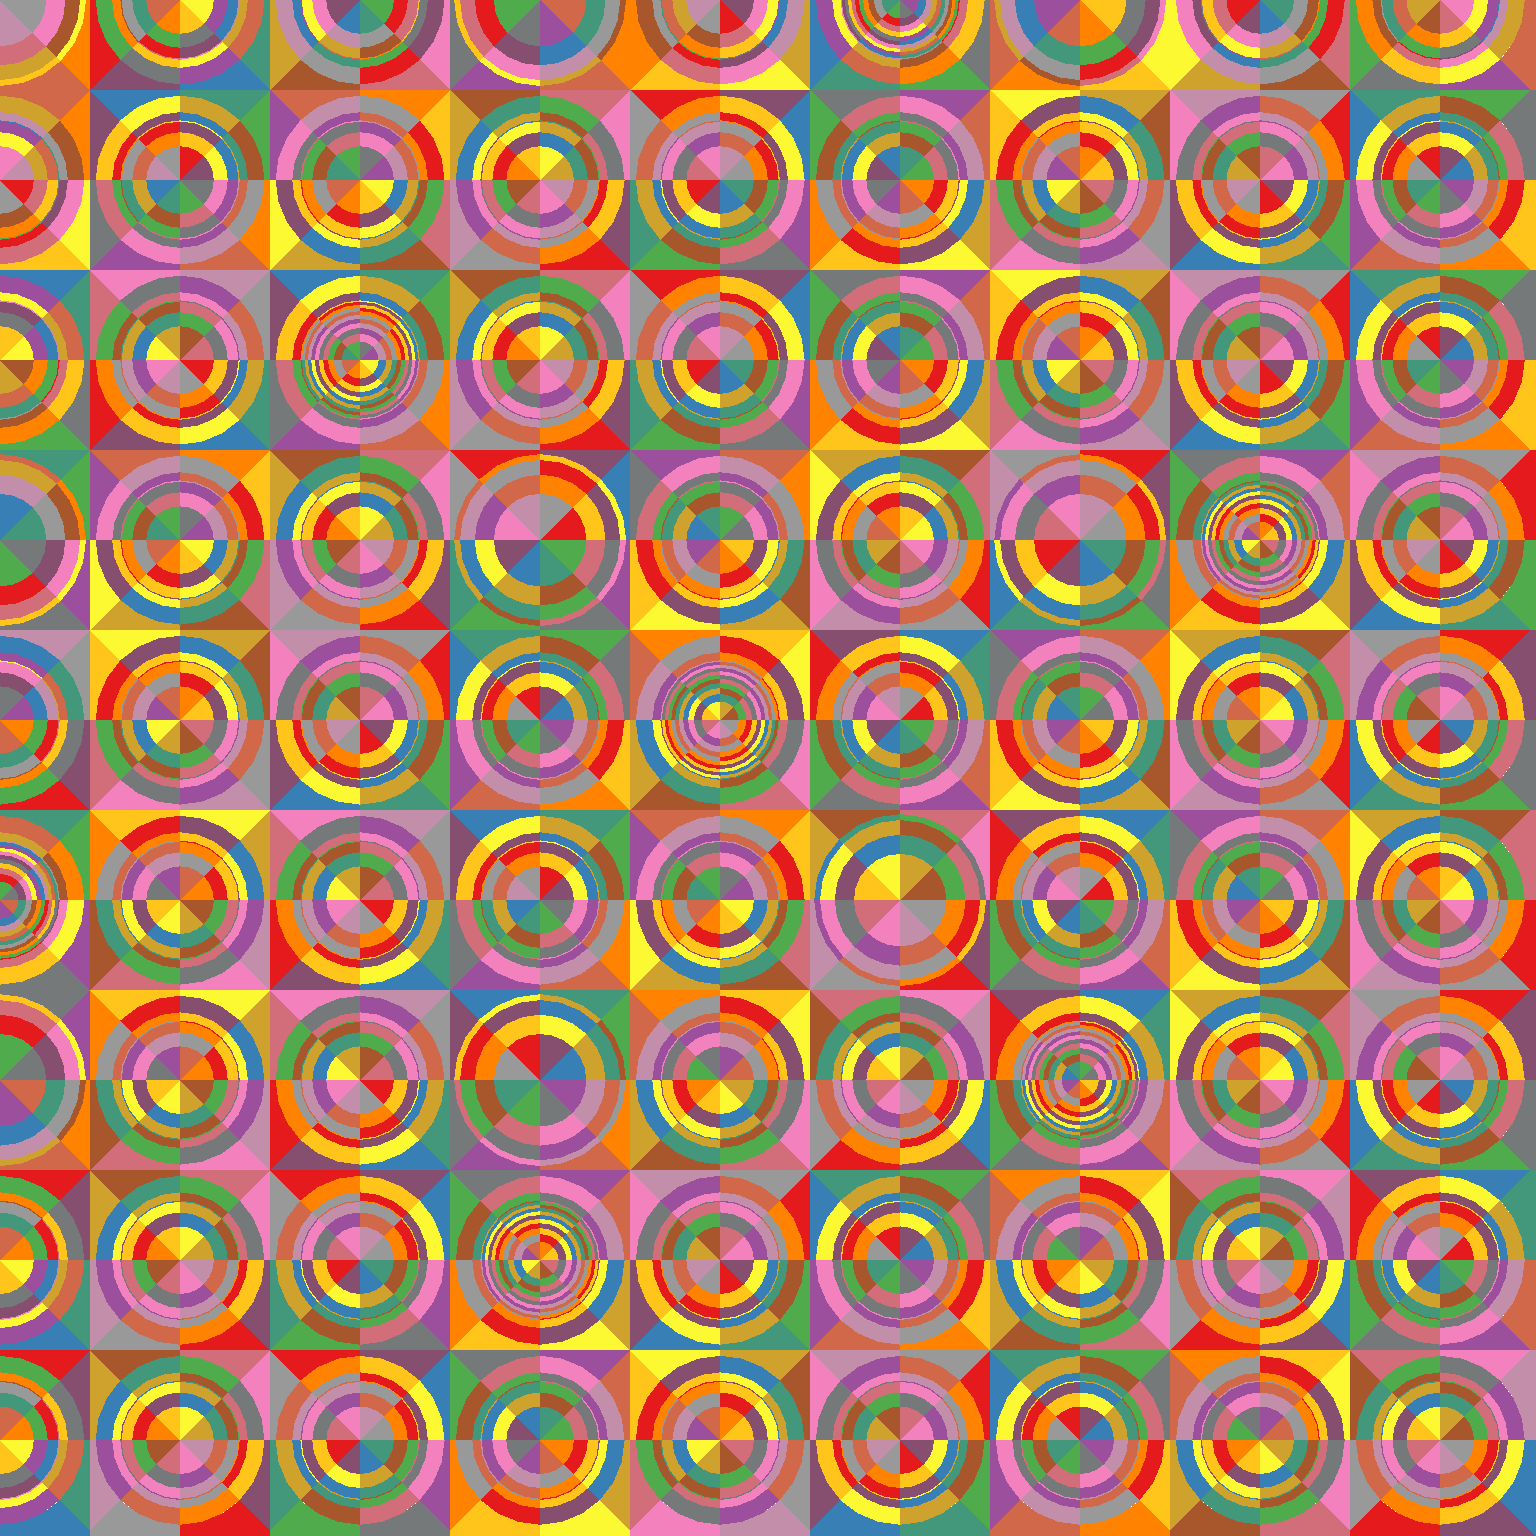
\includegraphics[width=\linewidth]{\figpath/lattice/2p/default.png}
                        \caption{Default lattice (2p) mesh\\\centering(4282 cells)}
                    \end{subfigure}%
                    ~
                    \begin{subfigure}[t]{0.40\linewidth}
                        \centering
                        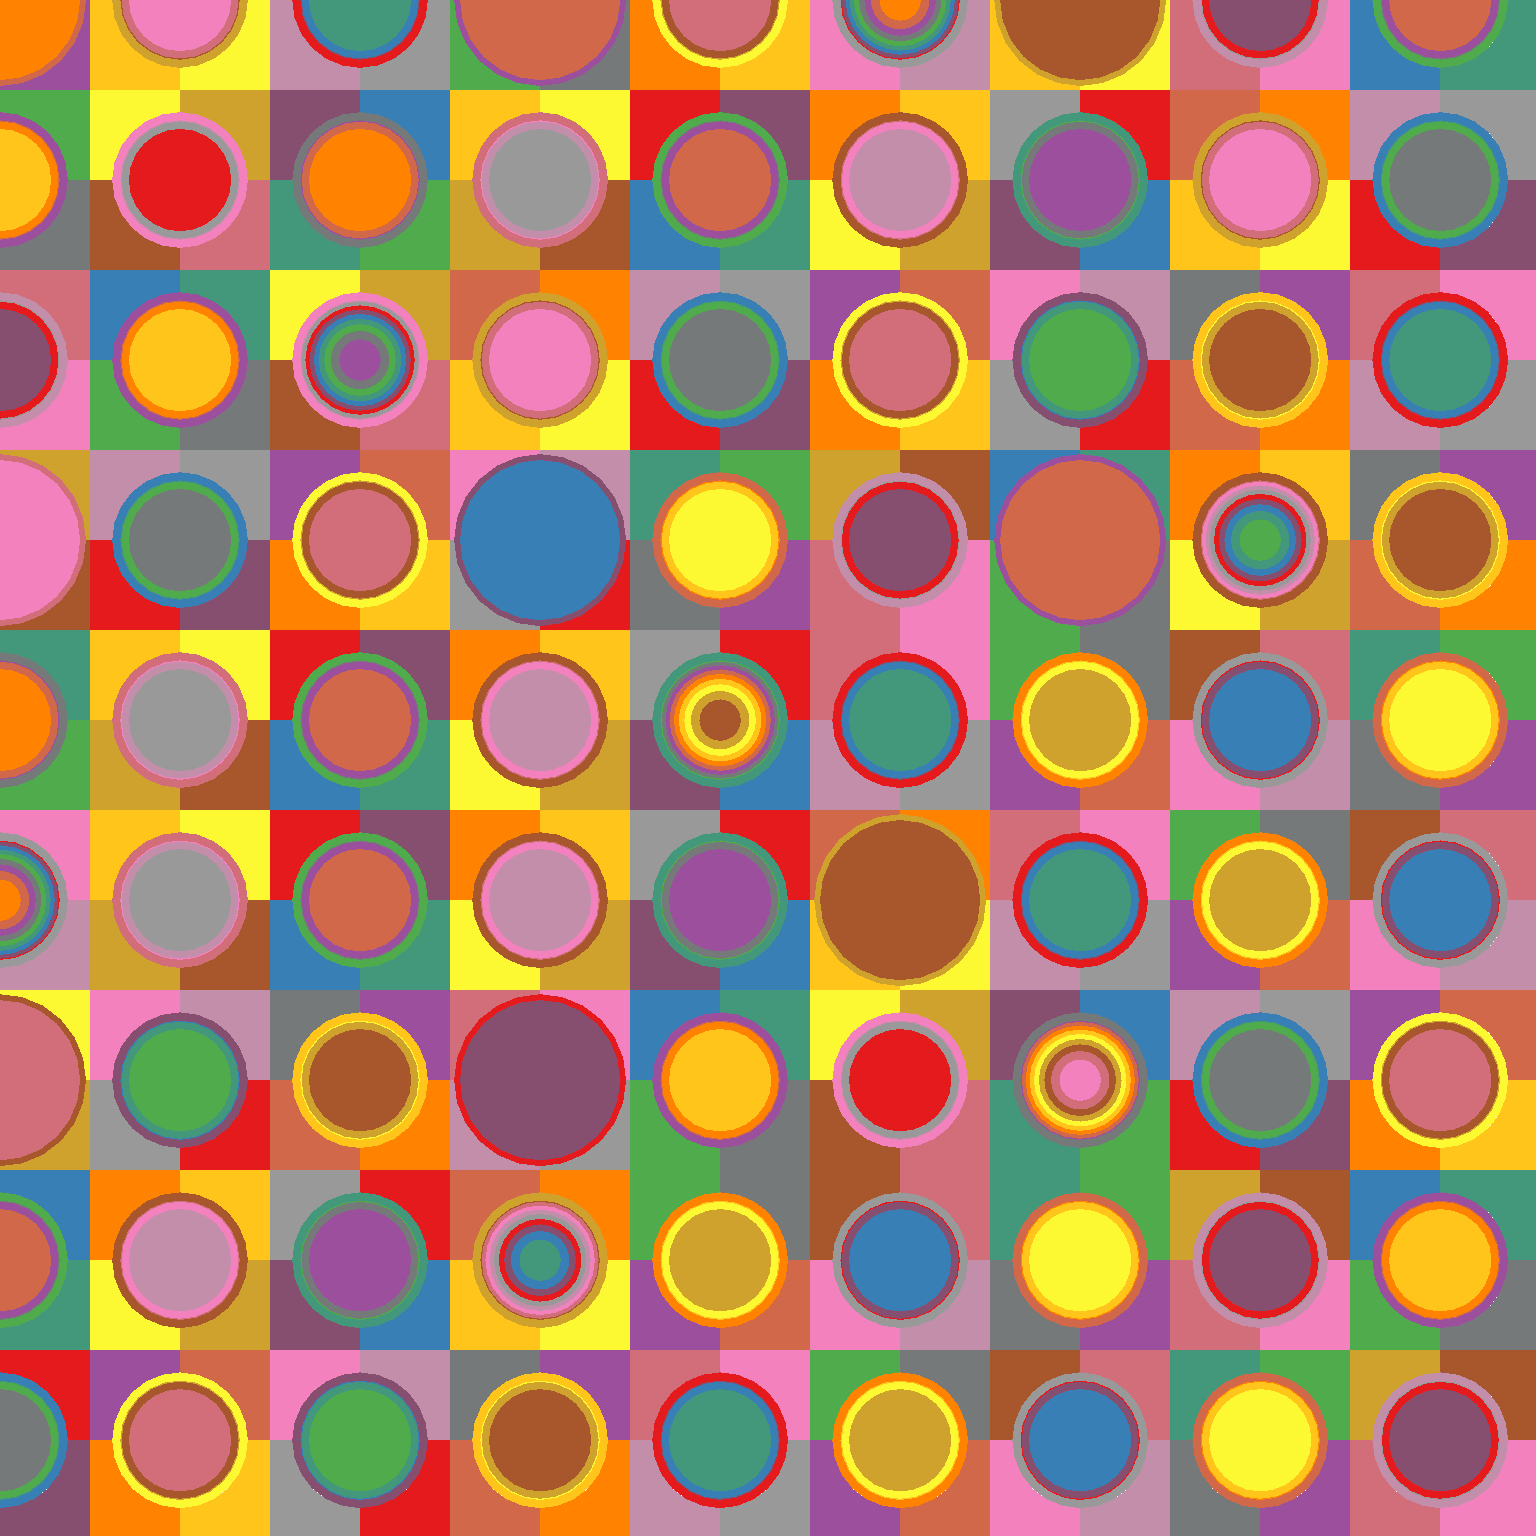
\includegraphics[width=\linewidth]{\figpath/lattice/2p/coarse.png}
                        \caption{Coarse lattice (2p) mesh\\\centering(637 cells)}
                    \end{subfigure}
                \end{minipage}
                \caption{Current default and coarse meshes for pin and lattice (2P) calculations.}
                \label{fig:Results:LSA:Depletion:Meshes}
            \end{figure}
            \begin{figure}[h]
                \centering
                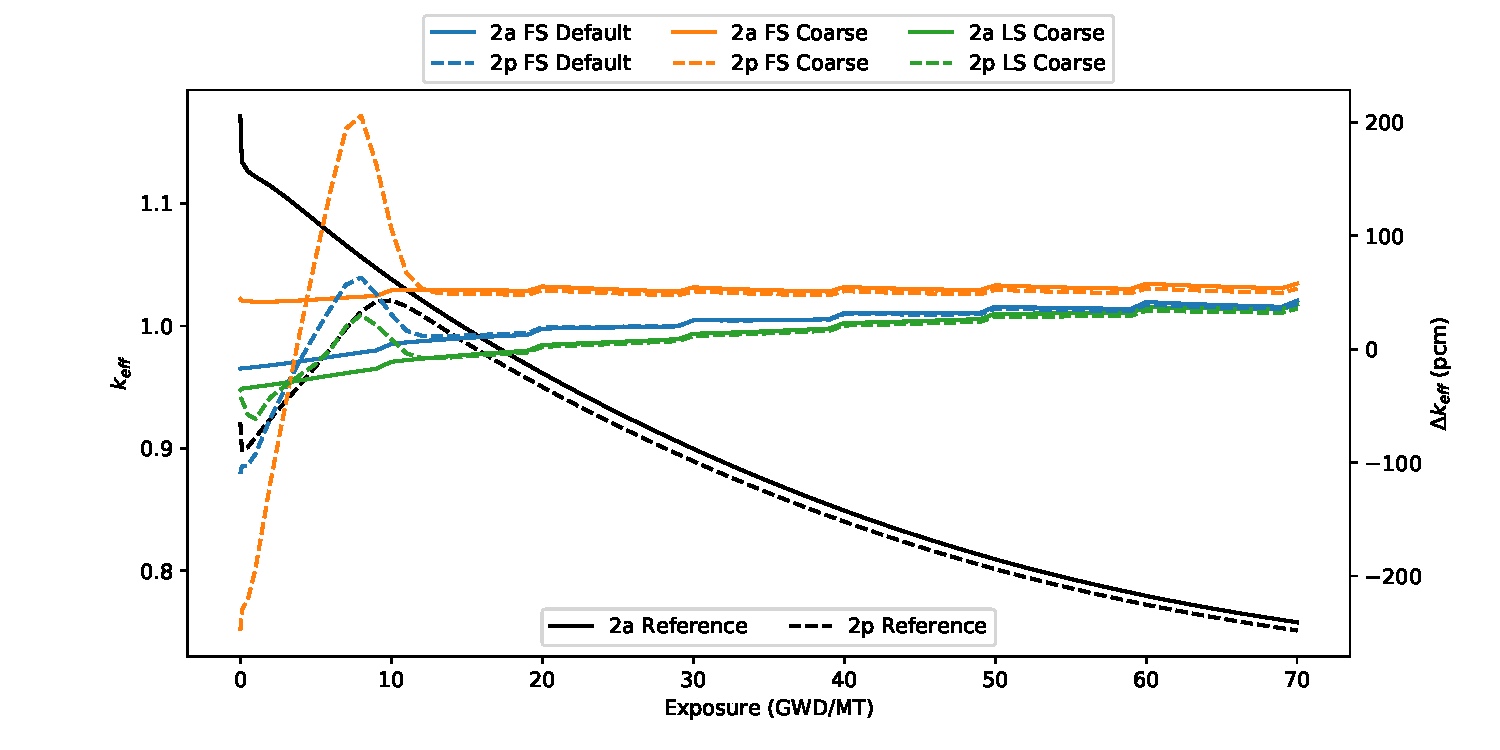
\includegraphics[width=0.85\linewidth]{\figpath/lattice/2p/lattice-depl-summary.pdf}
                \caption{Eigenvalue reference values and differences for default, and coarse mesh calculations throughout isotopic depletion of VERA problems 2A and 2P up to 70 MWD/kgHM.}
                \label{fig:Results:LSA:Lattice Depletion Results}
            \end{figure}
        }
        \subsection{3-D Assembly with T/H Feedback}{\label{ssec:Results:LSA:3D Assembly with T/H Feedback}
            The final case examined in this work was a single 3D assembly with \ac{TH} feedback: VERA problem 6 \cite{VERAProblems}.
            This case demonstrates that a coarser mesh can be used with the \ac{LSMOC} solver in problems with \ac{TH} feedback and in the 2D/1D framework \cite{Collins2016}.
            Meshing parameters from the previous results were used in fuel and guide-tube elements.
            The lower and upper plates and nozzles are meshed as rectilinear grids in MPACT; these were able to be coarsened to 0.42$\times$0.42 cm$^2$ sized elements.

            This case was run with the default and coarse meshes with the \ac{FSMOC} and \ac{LSMOC} solvers.
            Each calculation was compared against a finely meshed case run with the \ac{LSMOC} solver.
            The same angular quadratures were used in these assembly cases as the lattice cases, but a ray-spacing of 0.03 cm was used for the cases on the default and coarse meshes.
            Results are summarized in \cref{tab:Results:LSA:Assembly Results}.

            \Cref{tab:Results:LSA:Assembly Results} shows that the \ac{LSMOC} solver on the coarse mesh is at least as accurate as the \ac{FSMOC} solver on the current default mesh.
            Although the \ac{LSMOC} has lower total run-times, by about 6.5\%, these times cannot be directly compared due to the difference in number of outer iterations.
            This difference in iterations is likely caused by false convergence due to the oscillatory convergence observed in problems with \ac{TH} feedback and \ac{CMFD} acceleration \cite{Kochunas2017}.
            Scaling times by the number of outer iterations is also not a fair comparison because CMFD acceleration and CTF take significantly longer during the first several iterations.
            A fairer comparison is to instead compare the time of the default \ac{FSMOC} solver at 9 outer iterations to the \ac{LSMOC} solver: 392.99 seconds.
            This still indicates that the \ac{LSMOC} solver decreases run-times by about 4\%, and reduces memory usage by 21\%.
            This increased efficiency is significantly lower than in the previous results, though this is not surprising, as \ac{MOC} accounts for less than 5\% of the total run-time in this case.
            \begin{table}[h]
                \centering
                \caption{Eigenvalue and pin power comparison results for VERA problem 6.}
                \label{tab:Results:LSA:Assembly Results}
                \begin{tabular}{rrrr}
                                                & FS Default & FS Coarse & LS Coarse\\\toprule
                    $\Delta k_\text{eff}$ (pcm) &  33.54     & 108.74    & 13.22\\
                    RMS Pin Power Diff. (\%)    &   0.19     &   0.45    &  0.03\\
                    Max Pin Power Diff. (\%)    &   0.43     &   0.91    &  0.10\\
                    Time (s)                    &   403.7    & 388.1     & 376.2\\
                    Outer Iterations            &   11       & 11        & 9\\
                    Memory (MB)                 & 8398.4     & 6507.6    & 6583.0\\\bottomrule
                \end{tabular}
            \end{table}
        }
        \subsection{Summary}{\label{ssec:Results:LSA:Summary}
            Results have indicated that in multiphysics calculations (isotopic depletion and \ac{TH} feedback) \ac{LSMOC} solvers still allow for significant reduction in the computational mesh.
            In cases with isotopic depletion, the reformulated \ac{LSMOC} \cite{Fitzgerald2019} leads to significant runtime and memory advantages of \ac{FSMOC} solvers.
            However, in cases with \ac{TH} feedback, runtime is dominated by the \ac{TH} feedback solve; use of the \ac{LSMOC} leads to significant reduction in memory, but not runtime.

            Previous studies have indicated that the \ac{LSMOC} solvers allow for coarser meshes in 3-D single-physics (neutronics) calculations, leading to significant runtime advantages over the \ac{FSA} \cite{Boyd2014,Gunow2018}.
            The initial results of this work have indicated that the reformulated method allows for coarser meshes in multiphysics calculations in 2-D; this leads to the expectation that the reformulated \ac{LSMOC} will lead to runtime and memory advantages in 3-D multiphysics calculations.
            This remains as future work to be included as part of this thesis.

            Additionally, these initial results only present results for isotropic scattering cases, and should be generalized to include anisotropic sources.
            2-D and 3-D core-depletion calculations should also be performed to verify the mesh parameters found from this work.
        }
    }
    \section{2-D Macroband}{\label{sec:Results:2-D Macroband}
        Part of this thesis work is the extension of the macroband (\cref{sec:RT:Macroband}) ray-tracing method to three-dimensional transport problems.
        While 2-D macroband has been implemented and tested in previous studies \cite{Petkov1998,Yamamoto2005,Fevotte2007,Yamamoto2008}, to the best of the author's knowledge, no study has been performed for 3-D calculations.
        In 2-D, the macroband method allows for coarser ray-spacing with maintained accuracy leading to more efficient \ac{MOC} calculations; the expectation is that by extending this method to 3-D, ray-spacing can be reduced in both radial and axial directions, leading to a more significant increase in efficiency.

        As part of this thesis work, development of a macroray (\cref{ssec:RT:Macroray}) \ac{MOC} transport solver library is being implemented in MPACT.
        As \acp{GPU} have become more prevalent in parallelizable scientific computation, this \ac{MOC} library is being implemented with the Kokkos library \cite{Kokkos}; the Kokkos library allows for performant-portable code to run efficiently on both \ac{CPU} and \ac{GPU}.
        This has been the focus of recent work, and the \ac{MOC} library is still in early stages.
        The current form of the library uses the angle-dependent sub-boundary averaging technique for approximating angular flux on subsystem boundaries, as described by \citet{Liu2014}.
        Some initial results have been generated for a 2-D pin-cell, in order to help verify previous results on the macroband method.

        Initial tests have been performed on a single 2-D \acs{UO2} pin-cell from the c5g7 benchmark.
        Calculations were run using a range of ray-spacings, on a coarse mesh, with the linear source solver.
        Each calculation was run with the \ac{MRT}, Macroband with uniform spacing, and Macroband with Gauss-Legendre spacing.
        Initial results are shown in \cref{fig:Results:Macroband:EigenvalueComparisons,fig:Results:Macroband:EigenvalueError,fig:Results:Macroband:EigenvalueError vs nsegs}.

        One interesting thing to note, is that the \ac{MRT} ray-tracing methods converge to a different result as the ray-spacing is refined.
        This is likely due to the perturbation of the azimuthal quadrature caused by the \ac{DNPL} requirement of \ac{MRT}.
        It is also interesting to note, that the macroband method with Gauss-Legendre spacing seems to have better accuracy than the \ac{MRT} method; though in this case error is small, it will be useful to see results for a more realistic (51-group) pin-cell calculation.
        However, as previous studies have indicated \cite{Yamamoto2005}, the macroband method with uniform ray-spacing within each band seems to perform worse than the traditional ray-tracing techniques.

        \begin{figure}[h]
            \centering
            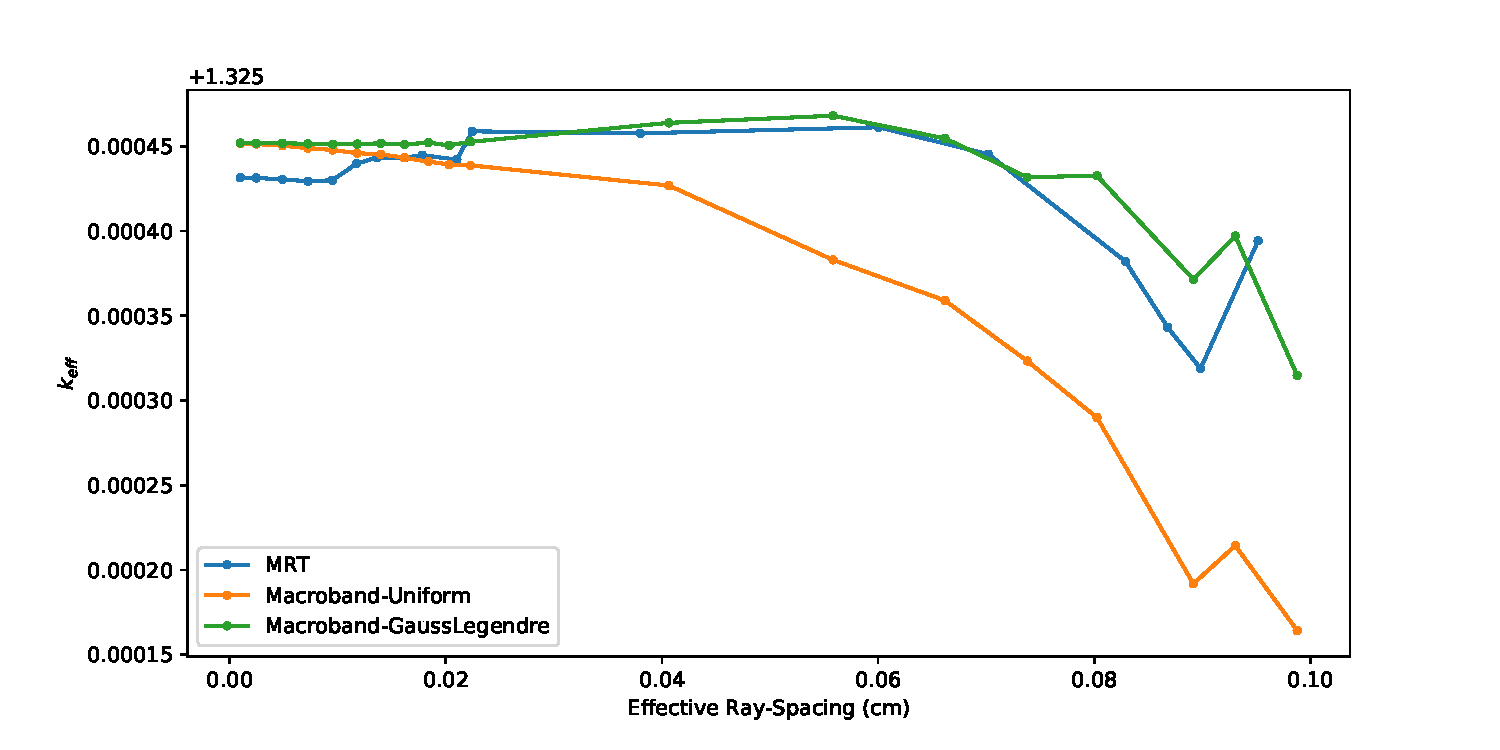
\includegraphics[width=0.65\linewidth]{\figpath/Macroband/EigenvalueComparisons}
            \caption{Eigenvalue comparisons for the different ray-tracing methods over a range of ray-spacings.}
            \label{fig:Results:Macroband:EigenvalueComparisons}
        \end{figure}
        \begin{figure}[h]
            \centering
            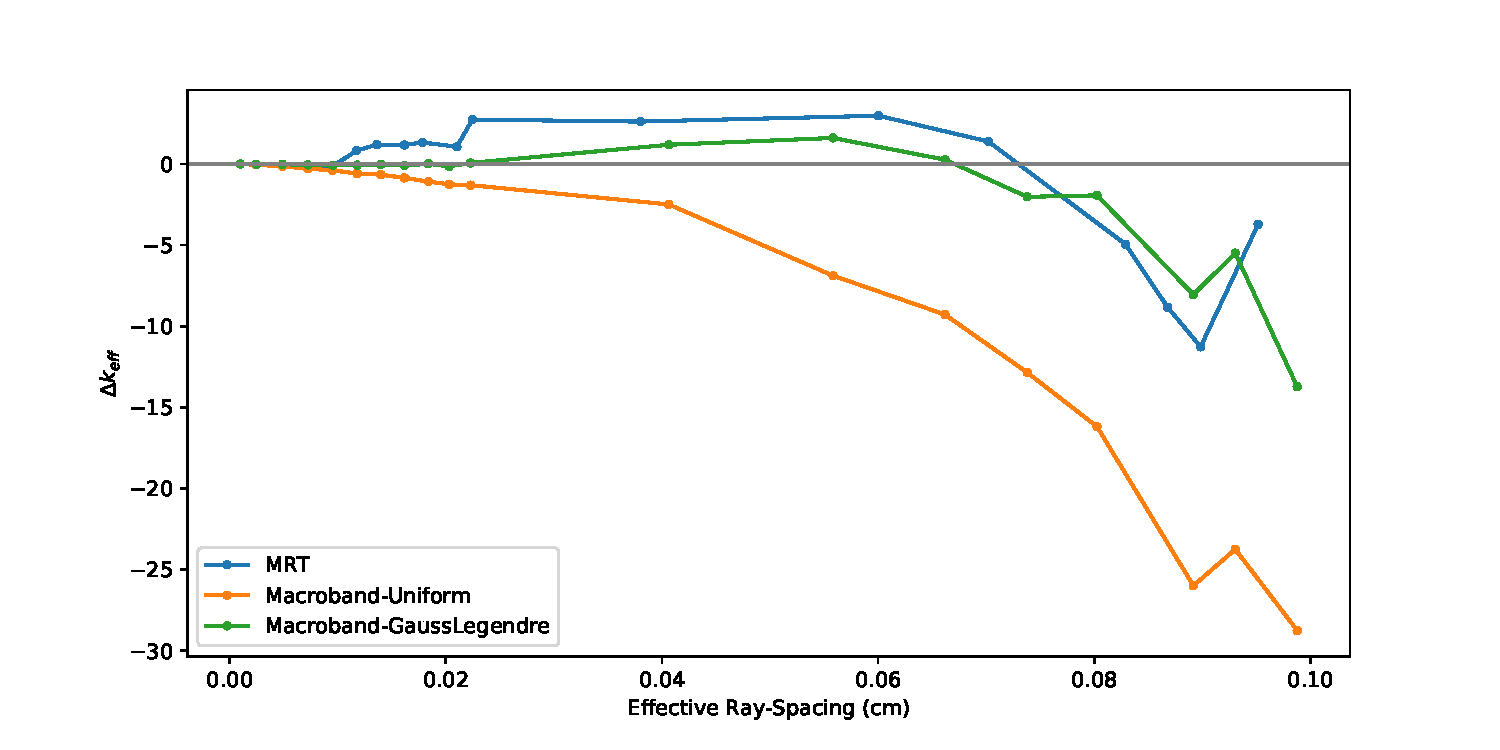
\includegraphics[width=0.65\linewidth]{\figpath/Macroband/EigenvalueError}
            \caption{Eigenvalue errors (relative to finest ray-spacing of that ray-tracing method) for each ray-tracing method over a range of ray-spacings.}
            \label{fig:Results:Macroband:EigenvalueError}
        \end{figure}
        \begin{figure}[h]
            \centering
            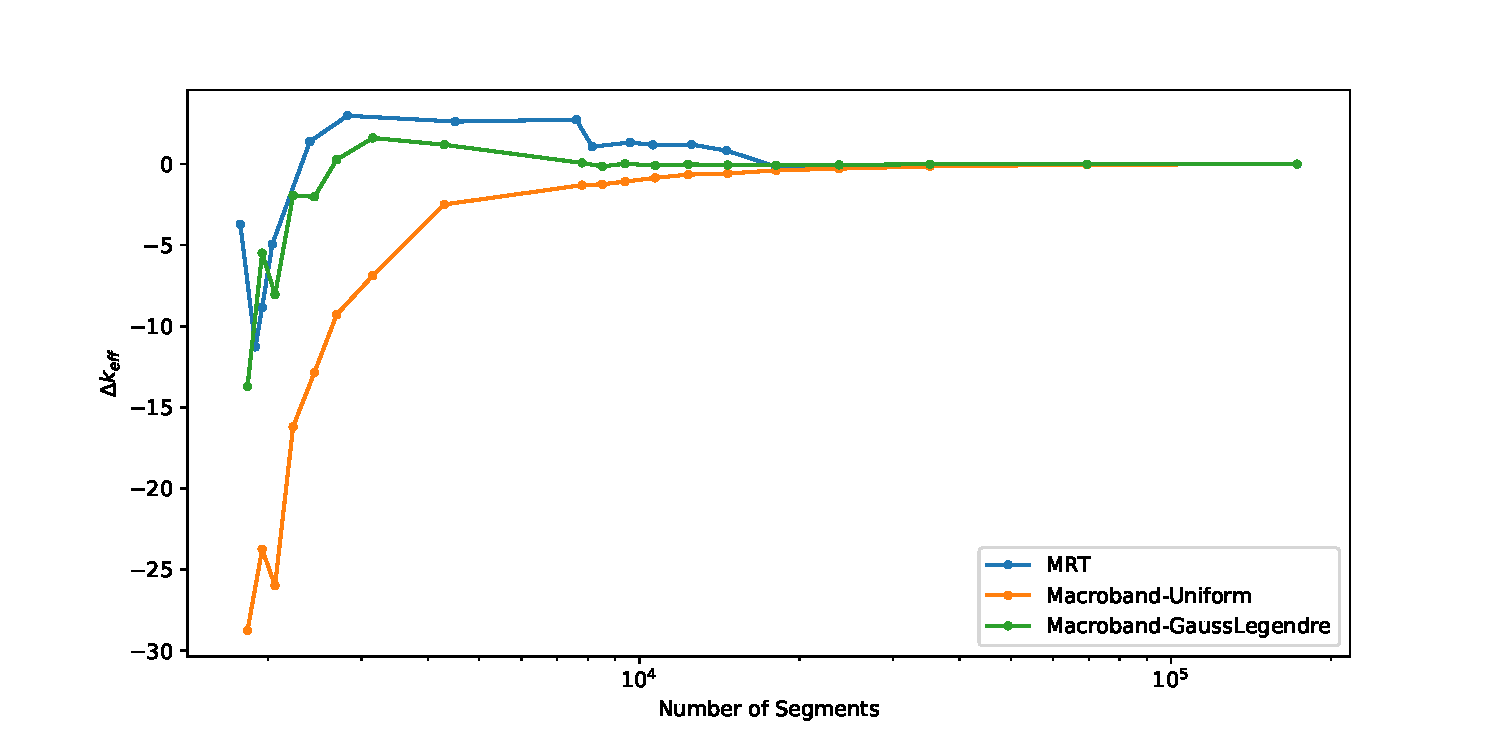
\includegraphics[width=0.65\linewidth]{\figpath/Macroband/ErrorVsNsegs}
            \caption{Eigenvalue errors (relative to finest ray-spacing of that ray-tracing method) for each ray-tracing method as a function of the number of track-segments.}
            \label{fig:Results:Macroband:EigenvalueError vs nsegs}
        \end{figure}

        A visualization of generated rays for this pin-cell are shown in \cref{fig:Results:Macroband:Rays}.
        Each of the macroband methods has obvious ``clustering'' effects near the small surfaces in the computational mesh, this is obvious in the azimuthal divisions in the moderator region outside the pin.
        This clustering is expected, as the macroband method will guarantee rays to pass through these surfaces, unlike the \ac{MRT}.
        Although this may not have significant effect in this case, it may when larger lattice cases are considered, particularly with respect to finely meshed strong absorbers.
        It is also interesting to observe that in the macroband with uniform spacing method, there seem to be concentric patterns where many rays intersect; it may be possible to remove these patterns by using a mobile-chord method within each macroband.

        \begin{figure}[h]
          \centering
          \begin{subfigure}[t]{0.45\linewidth}
            \centering
            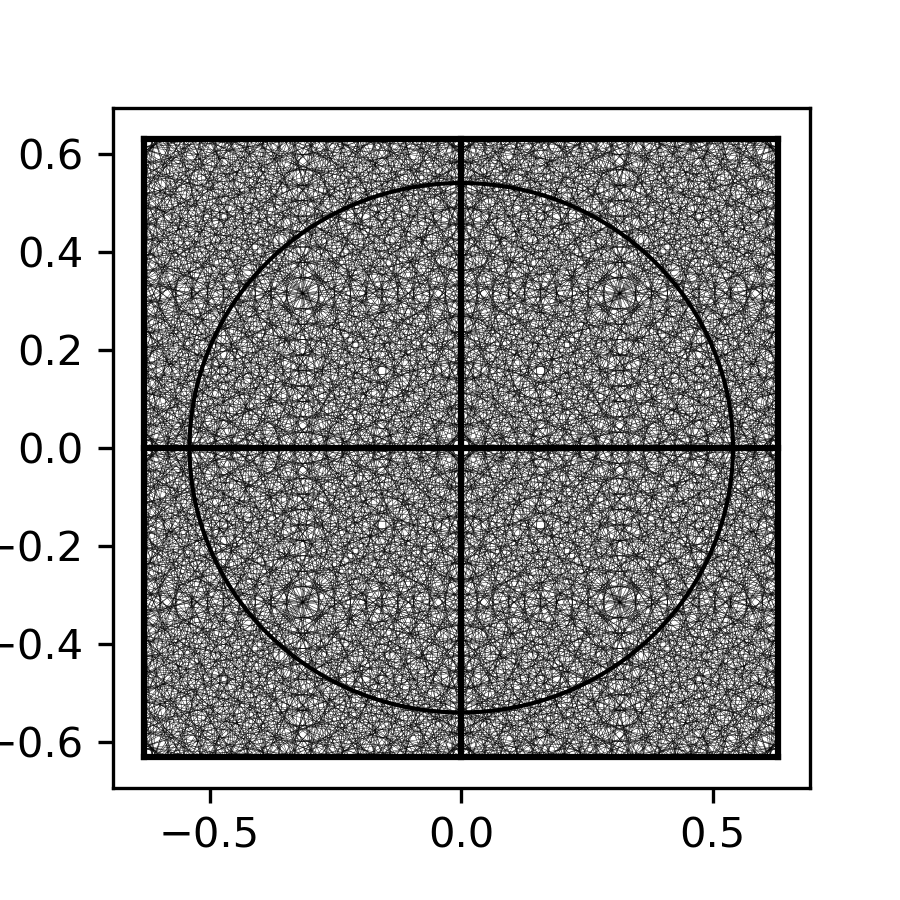
\includegraphics[width=\linewidth]{\figpath/Macroband/MRT_Rays}
            \caption{MRT}
            \label{fig:Results:Macroband:Rays:MRT}
          \end{subfigure}
          \begin{subfigure}[t]{0.45\linewidth}
            \centering
            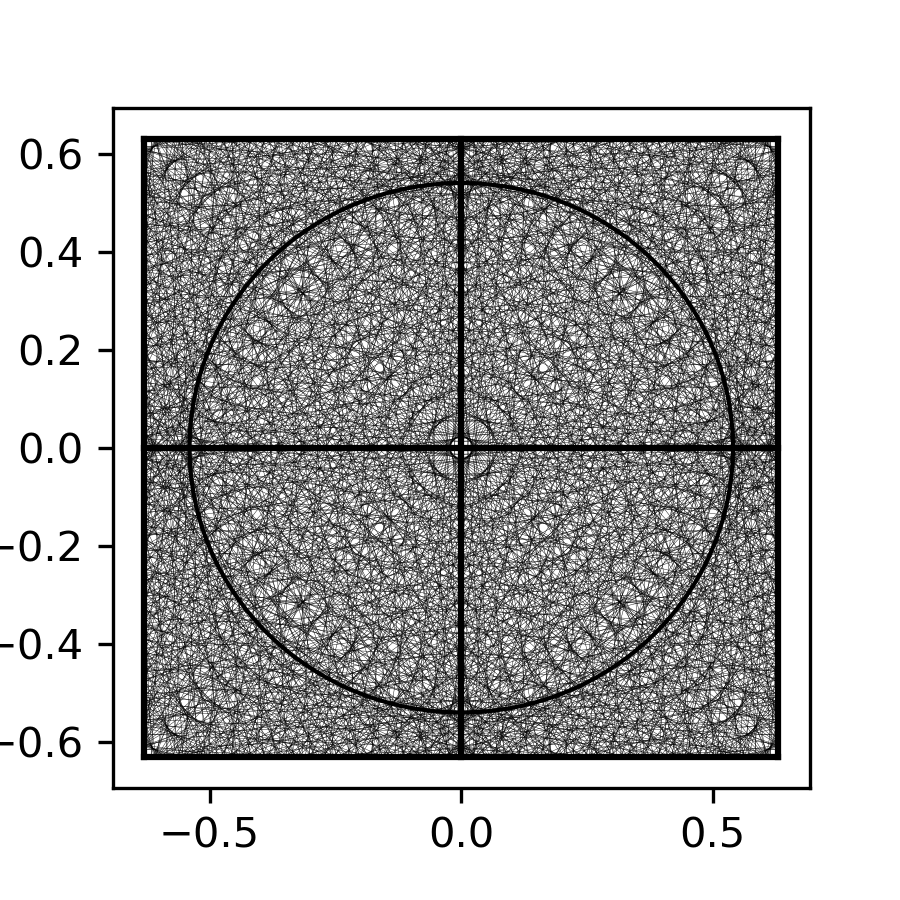
\includegraphics[width=\linewidth]{\figpath/Macroband/MBU_Rays}
            \caption{Macroband-Uniform}
            \label{fig:Results:Macroband:Rays:MBU}
          \end{subfigure}
          \begin{subfigure}[t]{0.45\linewidth}
            \centering
            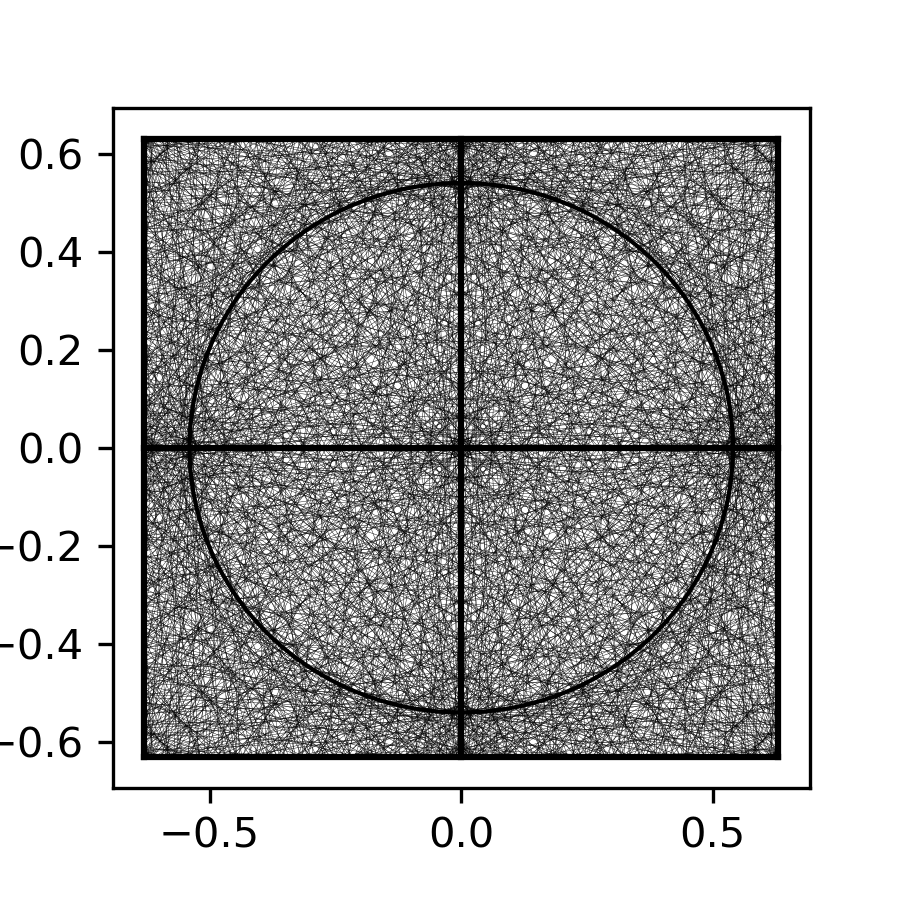
\includegraphics[width=\linewidth]{\figpath/Macroband/MBGL_Rays}
            \caption{Macroband-Gauss-Legendre}
            \label{fig:Results:Macroband:Rays:MBGL}
          \end{subfigure}
          \caption{Visualization of generated rays for an input spacing of 0.05 cm for each ray-tracing method.}
          \label{fig:Results:Macroband:Rays}
        \end{figure}
    }
    %%%%%%%%%%%%%%%%%%%%%%%%%%%%%%%%%%%%%%%%%%%%%%%%%%%%%%%%%%%%%%%%%%%%%%%%%%%%%%
    % Future work
    %%%%%%%%%%%%%%%%%%%%%%%%%%%%%%%%%%%%%%%%%%%%%%%%%%%%%%%%%%%%%%%%%%%%%%%%%%%%%%
    \section{Future work}{\label{sec:Results:Future work}
        The main contributions of this thesis work are the improved \ac{LSMOC}, the macroray ray-tracing techniques, and an improved spatial decomposition scheme, with application toward improving the efficiency of three-dimensional \ac{MOC} calculations.
        Thus far, 2-D studies have been performed on the \ac{LSMOC} with and without multiphysics \cite{Ferrer2016,Fitzgerald2019}, and 3-D studies have been performed without multiphysics \cite{Gunow2018}.
        Future work in this thesis requires larger 2-D multiphysics calculations to be run to verify new default mesh parameters, as well as 3-D multiphysics calculations.

        Work on the spatial decomposition scheme has largely been completed.
        Studies have been performed for 2-D transport calculations, and load-balance has been analyzed for 3-D problems \cite{Fitzgerald2019a}.
        The 2-D transport calculations revealed that some alignment of the spatial domains will have benefits in iteration convergence due to re-entrant flux.
        This indicates that for 3-D calculations, the axially and radially aligned decomposition schemes are likely to have an additional advantage not observed from load-balance results.

        Finally, implementation of the macroray based \ac{MOC} library is currently in progress.
        Several steps are still required for this implementation to be completed: calculations of current for \ac{CMFD} calculations, generalization to 3-D rays, multi-pin calculations, and anisotropic scattering.
        Studies should be performed on two-dimensional transport problems.
        A repetition of the lattice cases run in \cref{sec:Results:2-D Linear Source} should be run with each of the ray-tracing methods in 2-D calculations; this is to verify our treatment of interface conditions, as well as demonstrate the advantage in cases with strong absorbers.
        Additionally, as the methods are extended to three-dimensional problems, a scaling study of ray and segment requirements vs accuracy should be performed on a small problem.
        This study shall require investigation into the effect of directional quadrature modularization.

        An approximate outline of future activities is outlined in \cref{fig:Implementation Plan}.
        \begin{figure}[h]
            \centering
            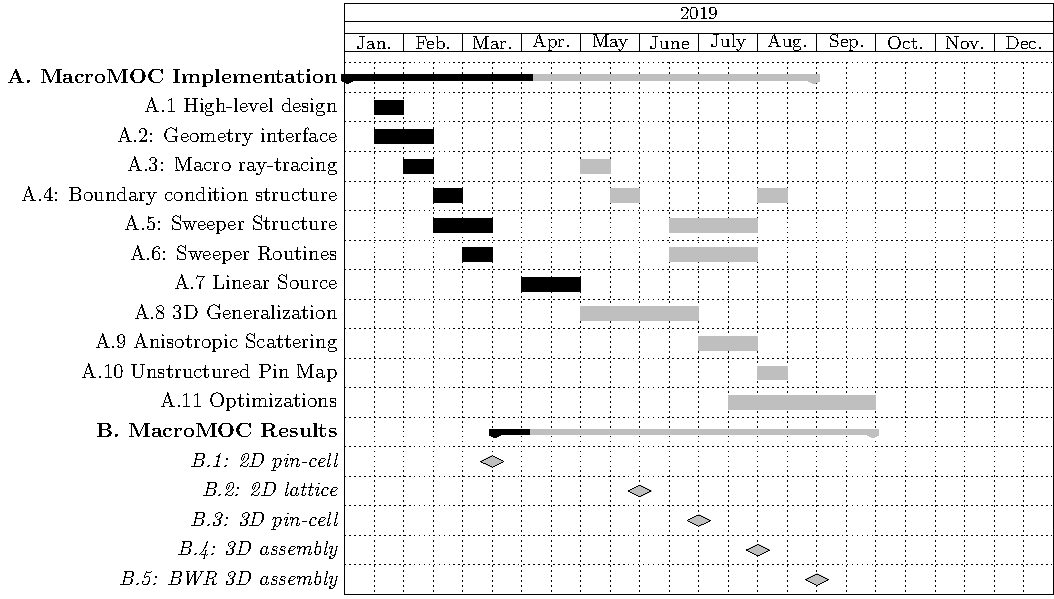
\includegraphics[width=\linewidth]{\figpath/plan/ganttChart.pdf}
            \caption{Possible plan for implementation of macroray \ac{MOC} library.}
            \label{fig:Implementation Plan}
        \end{figure}


    }
    % References
    % \printbibliography
}
    \printbibliography
    % \appendix
    %     \chapter{Spatial Decomposition}{\label{ch:Spatial Decomposition in MPACT}
    %         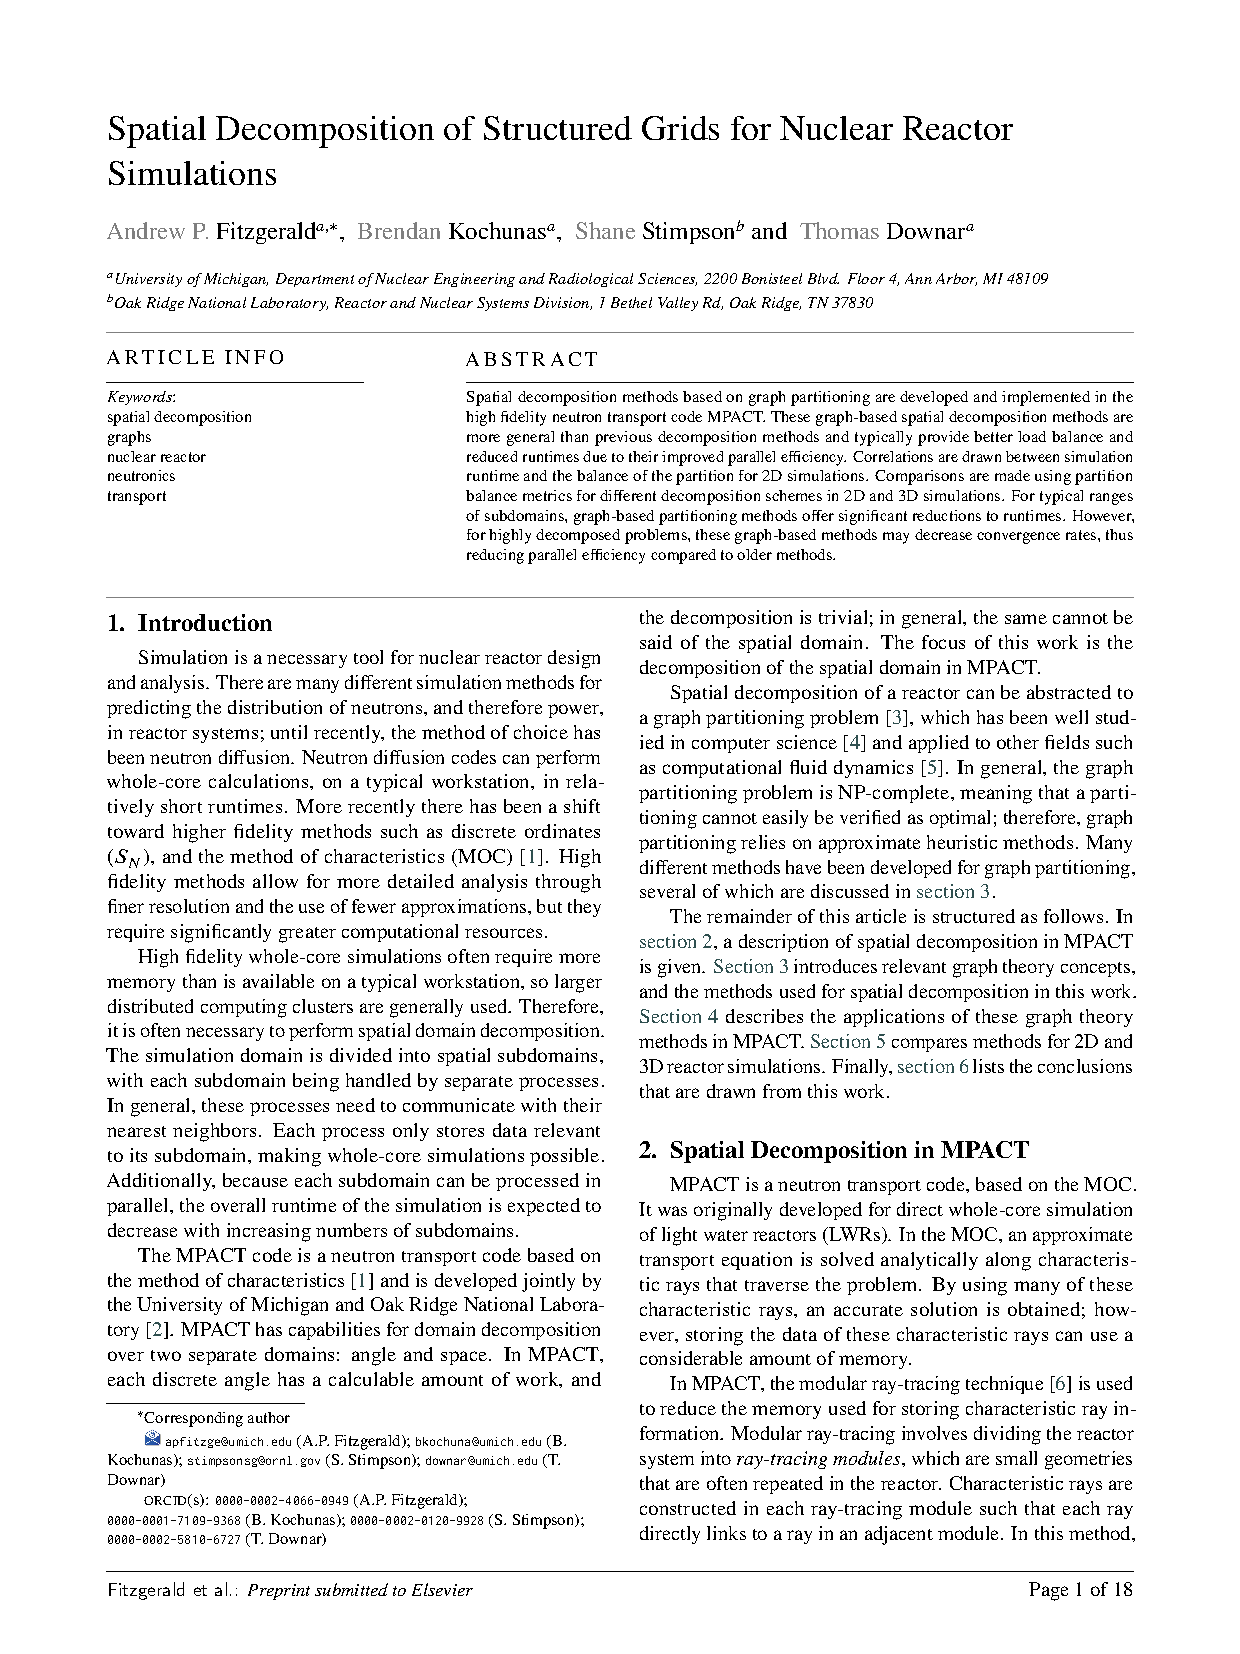
\includepdf[pages=-,scale=0.80,frame,pagecommand={}]{appendices/SpatialDecomposition/ANE-Manuscript.pdf}
    %     }
\end{document}